\chapter{AHTR One-Third Assembly Optimization Results}
\glsresetall
\label{chap:ahtr-assem-opt-results}
This chapter reports the \gls{AHTR} one-third assembly's \gls{ROLLO} optimization 
results. 
I vary the following \gls{AHTR} one-third assembly input parameters:
\begin{itemize}
    \item \gls{TRISO} packing fraction distribution ($\rho_{TRISO}(\vec{r})$)
    \item Total fuel packing fraction ($PF_{total}$)
    \item Coolant channel shape ($r_1, r_2, r_3, r_4,$ and $r_5$)
\end{itemize} 
Section \ref{sec:input-parameter-modeling} detailed how I vary these 
\gls{AHTR} one-third assembly's input parameters. 
I optimize the \gls{AHTR} one-third assembly for the following 
objectives:
\begin{itemize}
    \item Minimize total fuel packing fraction ($PF_{total}$)
    \item Minimize maximum one-third assembly temperature ($T_{max}$)
    \item Minimize fuel-normalized power peaking factor ($PPF_{fuel}$)
\end{itemize} 
Table \ref{tab:objectives} outlined these objectives and their motivation.
Chapter \ref{chap:method} detailed the methodology for \gls{AHTR} one-third 
assembly modeling and \gls{ROLLO} optimization. 

The subsequent sections outline the \gls{AHTR} one-third assembly's optimization 
simulations, describe the single-objective and multi-objective \gls{ROLLO} optimization 
simulations' results, report each simulation's computational cost, and discuss the 
results' significance.

\section{ROLLO AHTR One-Third Assembly Optimization Simulations Overview}
Table \ref{tab:assem-obj-breakdown} details the \gls{ROLLO} optimization problems 
explored in this chapter.
\begin{table}[htbp!]
    \centering
    \onehalfspacing
    \caption{\acrfull{ROLLO} simulations for optimizing \acrfull{AHTR}
    one-third assembly. $PF_{total}$: Total Fuel Packing Fraction, 
    $T_{max}$: Maximum one-third assembly Temperature, 
    $PPF_{fuel}$: Normalized Power Peaking Factor, $\rho_{TRISO}(\vec{r})$: 
    \gls{TRISO} packing fraction distribution}
	\label{tab:assem-obj-breakdown}
    \footnotesize
    \begin{tabular}{p{1.4cm}|p{1cm}|lllp{3cm}}
    \hline 
    \textbf{Num of Objs} & \textbf{Sim} & \textbf{Objectives} & \textbf{Constraints} &\textbf{Varying Parameters} & \textbf{Coupled Nuclear Software} \\
    \hline
    \multirow{9}{2cm}{1}& a-1a & \tabitem min($PF_{total}$) & \tabitem $k_{eff} \geq 1.38$ &\tabitem $\rho_{TRISO}(\vec{r})$ & OpenMC \\
    & & & & \tabitem $PF_{total}$ & \\
    \cline{2-6}
    & a-1b & \tabitem min($T_{max}$) & \tabitem $k_{eff} \geq 1.38$ &\tabitem $\rho_{TRISO}(\vec{r})$ & OpenMC, Moltres\\
    \cline{2-6}
    & a-1c & \tabitem min($PPF_{fuel}$) & \tabitem $k_{eff} \geq 1.38$ &\tabitem $\rho_{TRISO}(\vec{r})$ & OpenMC\\
    \cline{2-6}
    & a-1d & \tabitem min($PF_{total}$) & \tabitem $k_{eff} \geq 1.0$ &\tabitem Coolant channel shape & OpenMC \\
    & & & & \tabitem $PF_{total}$ & \\
    \cline{2-6}
    & a-1e & \tabitem min($T_{max}$) & \tabitem $k_{eff} \geq 1.38$ &\tabitem Coolant channel shape & OpenMC, Moltres\\
    \cline{2-6}
    & a-1f & \tabitem min($PPF_{fuel}$) & \tabitem $k_{eff} \geq 1.0$ &\tabitem Coolant channel shape & OpenMC\\
    \hline
    \multirow{6}{2cm}{2}& a-2a & \tabitem min($PF_{total}$) & \tabitem $k_{eff} \geq 1.38$ & \tabitem $\rho_{TRISO}(\vec{r})$ & OpenMC, Moltres\\
    & &\tabitem min($T_{max}$) & & \tabitem $PF_{total}$ & \\
    \cline{2-6}
    & a-2b & \tabitem min($PF_{total}$) & \tabitem $k_{eff} \geq 1.38$ & \tabitem $\rho_{TRISO}(\vec{r})$ & OpenMC\\
    & & \tabitem min($PPF_{fuel}$) & & \tabitem $PF_{total}$ & \\
    \cline{2-6}
    & a-2c & \tabitem min($T_{max}$) & \tabitem $k_{eff} \geq 1.38$ & \tabitem $\rho_{TRISO}(\vec{r})$ & OpenMC, Moltres\\
    & & \tabitem min($PPF_{fuel}$) & & & \\
    \hline
    \multirow{6}{2cm}{3}& a-3a &\tabitem min($PF_{total}$) & \tabitem $k_{eff} \geq 1.38$ & \tabitem $\rho_{TRISO}(\vec{r})$ & OpenMC, Moltres\\
    && \tabitem min($PPF_{fuel}$) & & \tabitem $PF_{total}$ & \\
    && \tabitem min($T_{max}$) & & & \\
    \cline{2-6}
    & a-3b &\tabitem min($PF_{total}$) & \tabitem $k_{eff} \geq 1.38$ & \tabitem $\rho_{TRISO}(\vec{r})$ & OpenMC, Moltres\\
    && \tabitem min($PPF_{fuel}$) & & \tabitem $PF_{total}$ & \\
    && \tabitem min($T_{max}$) & & \tabitem Coolant channel shape& \\
    \hline
    \end{tabular}
\end{table}
I first conducted single objective, single input parameter \gls{ROLLO} optimizations 
to understand the individual impacts of each objective on each input parameter. 
Their results will inform the multi-objective optimization simulation setup. 

Simulations are run on the Theta supercomputer at the Argonne Leadership Computing 
Facility under the Director's Discretionary Allocation Program 
\cite{noauthor_argonne_2022}. 
Section \ref{sec:assem-compute-cost} details each optimization simulation's computational 
cost.  

\section{AHTR One-Third Assembly: Single-Objective Optimization Results}
\label{sec:assem-one-obj}
This section reports the \gls{AHTR} one-third assembly's \gls{ROLLO} 
single-objective optimization results. 
Table \ref{tab:assem-obj-breakdown} summarized the one-objective simulations:
a-1a, a-1b, a-1c, a-1d, a-1e, and a-1f. 
In the following subsections, I describe the single-objective optimization results 
grouped by the minimized objective. 

If a single-objective optimization problem's objective converges earlier than the 
five generations I intended to run (determined in Section 
\ref{sec:multi-obj-hyperparameters}), I stop the simulation at that generation. 
Section \ref{sec:rollo-convergence} described how reactor designers use 
\gls{ROLLO} to determine problem convergence. 

\subsection{Objective: Minimize Total Packing Fraction ($PF_{total}$)}
\label{sec:assem-1-obj-pf}
This section reports results from the minimize total fuel packing fraction 
($PF_{total}$) single-objective optimization simulations: a-1a and a-1d. 
Simulation a-1a varies the $PF_{total}$ and \gls{TRISO} 
packing fraction distribution ($\rho_{TRISO}(\vec{r})$), and simulation a-1d varies 
the $PF_{total}$ and coolant channel shape ($r_1, r_2, r_3, r_4,$ and $r_5$). 

\subsubsection{Simulation a-1a: Variation of $PF_{total}$ and $\rho_{TRISO}(\vec{r})$}
Table \ref{tab:simulationa1a} shows simulation a-1a's optimization problem parameters. 
\begin{table}[htbp!]
    \centering
    \onehalfspacing
    \caption{Simulation a-1a Optimization Problem Parameters}
	\label{tab:simulationa1a}
    \footnotesize
    \begin{tabular}{l|p{5.3cm}}
    \hline 
    \multicolumn{2}{c}{\textbf{Single Objective: Simulation a-1a}} \\
    \hline 
    \textbf{Objectives} & Minimize $PF_{total}$ \\
    \hline 
    \textbf{Input Parameter Variations} & $0.05 \leq PF_{total} \leq 0.07$ \\
    & $\rho_{TRISO}(\vec{r})$: $0 \leq a \leq 2$, $0 \leq d \leq 2$\\
    & $\rho_{TRISO}(\vec{r})$: $0 \leq b \leq \frac{\pi}{2}$, $0 \leq e \leq \frac{\pi}{2}$\\
    & $\rho_{TRISO}(\vec{r})$: $0 \leq c \leq 2\pi$, $0 \leq f \leq 2\pi$\\
    \hline
    \textbf{Constraints} & $k_{eff} \geq 1.38$\\ 
    \hline 
    \textbf{Genetic Algorithm Parameters} & Population size: 128 \\
    & Generations: 3 \\
    \hline
    \end{tabular}
\end{table}

The one-third assembly's TRISO distribution is varied based on sine distributions, 
as described in Section \ref{sec:input-parameter-modeling}. 
If the simulation used the FHR benchmark equivalent $PF_{total} = 0.153$, at
certain sine distributions, some fuel cells would have $PF > 0.3$. 
OpenMC's random sequential packing algorithm becomes prohibitively slow at $PF > 0.3$, 
resulting in long runtimes. 
Therefore, I used $PF_{total} = 0.06$ because it is approximately the smallest 
$PF_{total}$ that enables $k_{eff} \geq 1.38$ and will avoid fuel cells with 
$PF > 0.3$ occurrences. 
I use $PF_{total} = 0.06$ for all optimization simulations that do not vary 
$PF_{total}$: a-1b, a-1c, a-1e, a-1f, and a-2c. 
I vary $PF_{total}$ between $0.05$ and $0.07$ for all optimization simulations 
that vary $PF_{total}$: a-1a, a-1d, a-2a, a-2b, a-3a, and a-3b.

Figure \ref{fig:assem-obj-1-pf-evol} shows the $PF_{total}$ evolution.
Figure \ref{fig:assem-obj-1-pf-final} shows four unique TRISO packing fraction 
distributions in the final generation with the most-minimized $PF_{total}$. 
Figure \ref{fig:assem-obj-1-pf-most-minimized} illustrates the \gls{AHTR} one-third 
assembly model with the most-minimized $PF_{total}$.
\begin{figure}[htbp!]
    \begin{subfigure}{\textwidth}
        \centering
        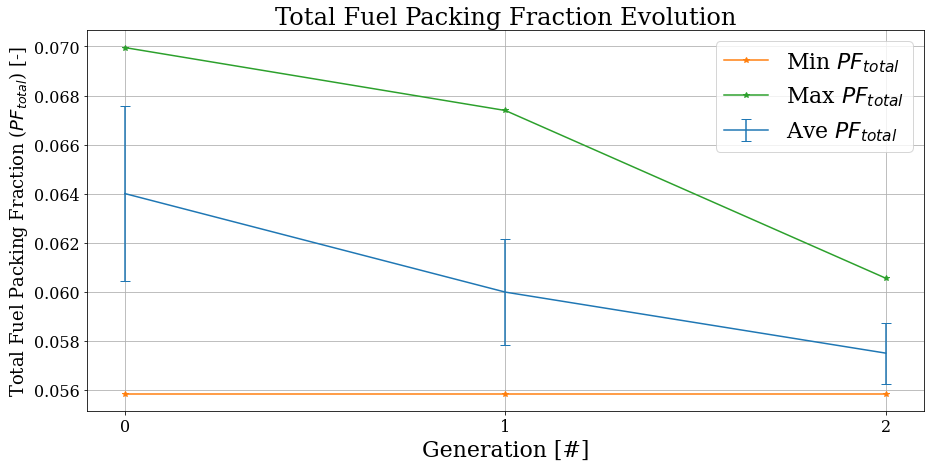
\includegraphics[width=\linewidth]{assem-obj-1-pf-evol.png}
        \caption{Minimum, average, and maximum $PF_{total}$ evolution.}
        \label{fig:assem-obj-1-pf-evol} 
    \end{subfigure}
    \begin{subfigure}{\textwidth}
        \centering
        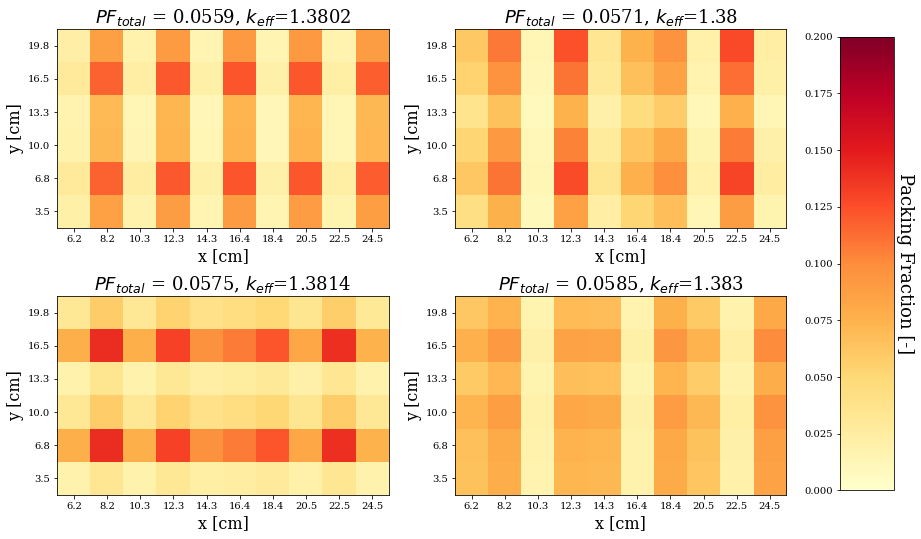
\includegraphics[width=\linewidth]{assem-obj-1-pf-final.png}
        \caption{TRISO packing fraction distribution for four unique reactor models with the 
        smallest $PF_{total}$ in the final generation.}
        \label{fig:assem-obj-1-pf-final} 
    \end{subfigure}
    \caption{Simulation a-1a -- ROLLO single-objective optimization to minimize total 
    fuel packing fraction ($PF_{total}$) in \gls{AHTR} one-third assembly. 
    Input parameters varied: $PF_{total}$, \gls{TRISO} packing fraction 
    distribution ($\rho_{TRISO}(\vec{r})$).}
    \label{fig:assem-obj-1-pf}
\end{figure}
\begin{figure}[htbp!]
    \ContinuedFloat
    \begin{subfigure}{\textwidth}
        \centering
        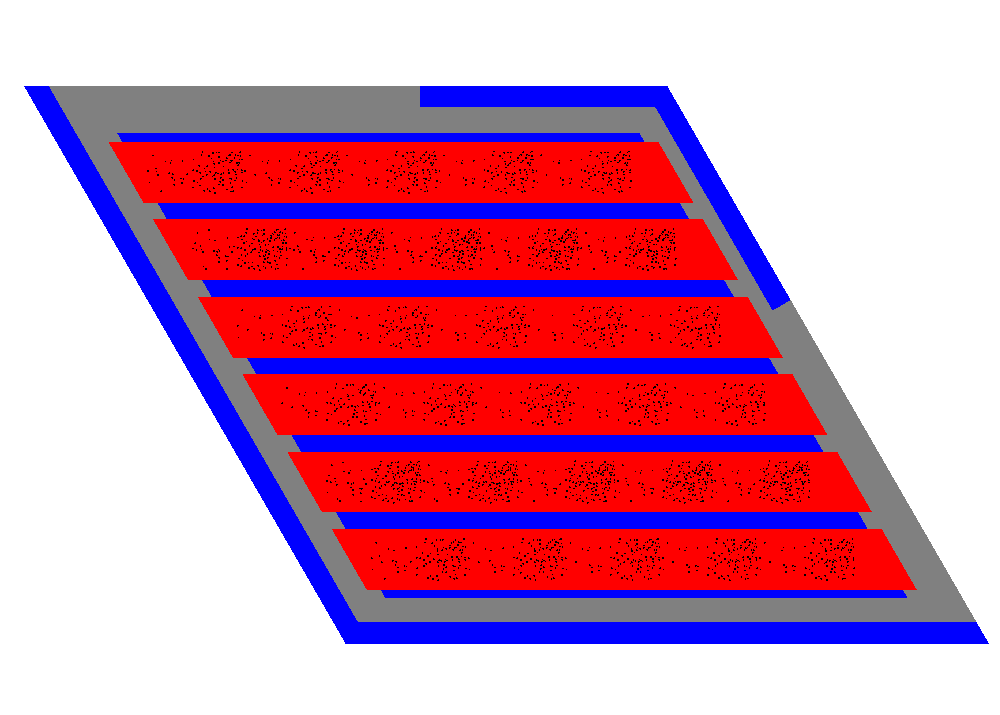
\includegraphics[width=0.7\linewidth]{assem-obj-1-pf-most-minimized.png}
        \caption{\gls{AHTR} one-third assembly model with the most-minimized 
        $PF_{total}$, corresponding to the first TRISO distribution in Figure 
        \ref{fig:assem-obj-1-pf-final}. The reactor model has $PF_{total}=0.0559$
        and $k_{eff}=1.3802$.}
        \label{fig:assem-obj-1-pf-most-minimized} 
    \end{subfigure}
    \caption{(contd.) Simulation a-1a -- ROLLO single-objective optimization to minimize total 
    fuel packing fraction ($PF_{total}$) in \gls{AHTR} one-third assembly. 
    Input parameters varied: total fuel packing fraction 
    ($PF_{total}$), \gls{TRISO} packing fraction distribution ($\rho_{TRISO}(\vec{r})$).}
\end{figure}

Figure \ref{fig:assem-obj-1-pf-evol} shows that the minimum and average $PF_{total}$ 
converged to approximately 0.057 in the final generation. 
In Figure \ref{fig:assem-obj-1-pf-final}, the four unique TRISO packing fraction 
distributions in the final generation that most-minimized $PF_{total}$ have various 
oscillating TRISO distribution patterns. 

The one-third assembly model with the most-minimized $PF_{total}$ has a 
$PF_{total} =0.0559$, an oscillating TRISO distribution along the 
x-axis and y-axis, and a packing fraction standard deviation of $0.04$ across the 
one-third assembly. 
Along the x-axis, the distribution peaks on the even fuel cell columns (at 8.2cm, 12.3cm, 
16.4cm, 20.5cm, and 24.5cm). 
The even columns have the largest y-axis variation of $\sim0.05$ with peaks of
$PF\approx0.12$.
The odd columns have the smallest y-axis variation of $\sim0.01$ with minimums of 
$PF\approx0.01$.
Along the y-axis, the distribution peaks on the 2nd and 5th fuel cell rows (at 6.8cm and 
16.5cm).
The 2nd and 5th row have the largest x-axis variation of $\sim0.10$ with peaks of 
$PF\approx0.12$. 
The middle 3rd and 4th rows have the smallest x-axis variation of $\sim0.06$ with 
minimums of $PF\approx0.01$.
Section \ref{sec:assem-discussion-pf} discusses the driving factors for the minimize 
$PF_{total}$ objective and explains simulation a-1a's most-minimized $PF_{total}$ 
oscillating TRISO distribution. 

\subsubsection{Simulation a-1d: Variation of $PF_{total}$ and Coolant channel shape}
Table \ref{tab:simulationa1d} shows simulation a-1d's optimization problem parameters. 
\begin{table}[htbp!]
    \centering
    \onehalfspacing
    \caption{Simulation a-1d Optimization Problem Parameters}
	\label{tab:simulationa1d}
    \footnotesize
    \begin{tabular}{l|p{6cm}}
    \hline 
    \multicolumn{2}{c}{\textbf{Single Objective: Simulation a-1d}} \\
    \hline 
    \textbf{Objectives} & Minimize $PF_{total}$ \\
    \hline 
    \textbf{Input Parameter variations} & $0.01<PF_{total}<0.04$ \\
    & coolant channel shape: $0.05<r_{1}<0.35$ \\
    & coolant channel shape: $0.05<r_{2}<0.35$ \\
    & coolant channel shape: $0.05<r_{3}<0.35$ \\
    & coolant channel shape: $0.05<r_{4}<0.35$ \\
    & coolant channel shape: $0.05<r_{5}<0.35$ \\
    \hline
    \textbf{Constraints} & $k_{eff} \geq 1.0$\\ 
    \hline 
    \textbf{Genetic Algorithm Parameters} & Population size: 64 \\
    & Generations: 2 \\
    \hline
    \end{tabular}
\end{table}

Figure \ref{fig:a-1d} shows the plots of coolant channel shape's 
$r_1, r_2, r_3, r_4,$ and $r_5$ values against $PF_{total}$. 
\begin{figure}[htbp!]
    \centering
    \begin{subfigure}{0.49\textwidth}
        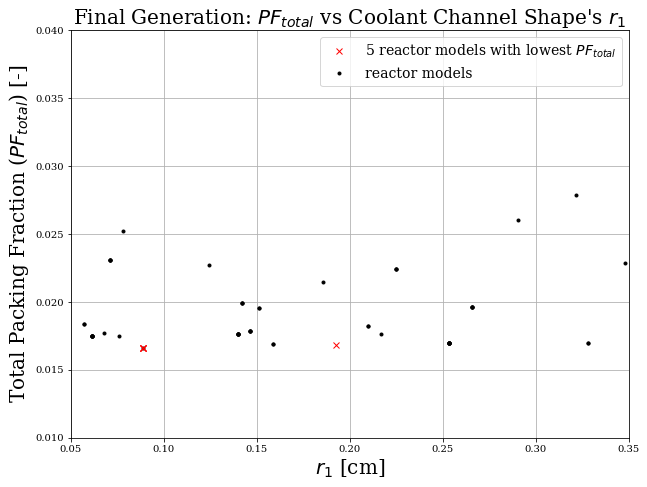
\includegraphics[width=\linewidth]{a-1d-r1.png}
        \caption{Plot of $PF_{total}$ against $r_1$.}
        \label{fig:a-1d-r1} 
    \end{subfigure}
    \begin{subfigure}{0.49\textwidth}
        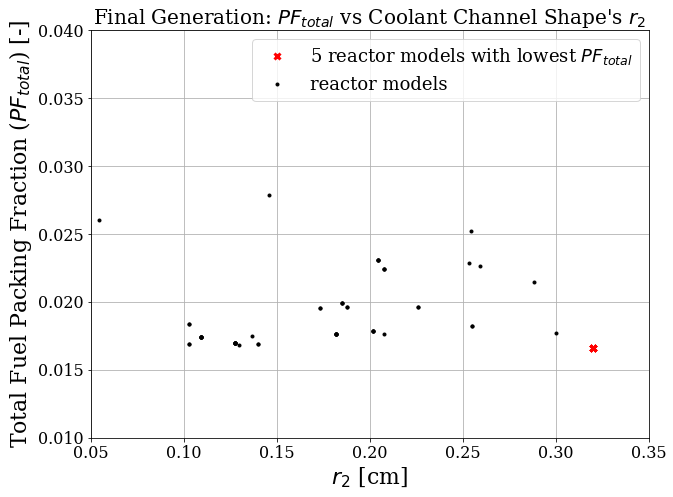
\includegraphics[width=\linewidth]{a-1d-r2.png}
        \caption{Plot of $PF_{total}$ against $r_2$.}
        \label{fig:a-1d-r2} 
    \end{subfigure}
    \begin{subfigure}{0.49\textwidth}
        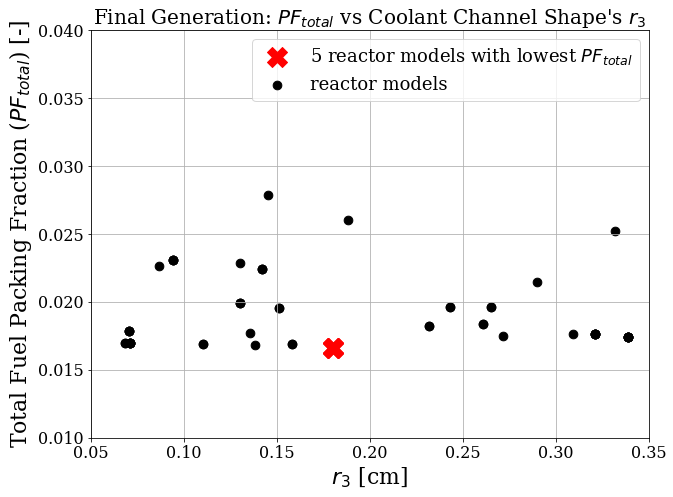
\includegraphics[width=\linewidth]{a-1d-r3.png}
        \caption{Plot of $PF_{total}$ against $r_3$.}
        \label{fig:a-1d-r3} 
    \end{subfigure}
    \begin{subfigure}{0.49\textwidth}
        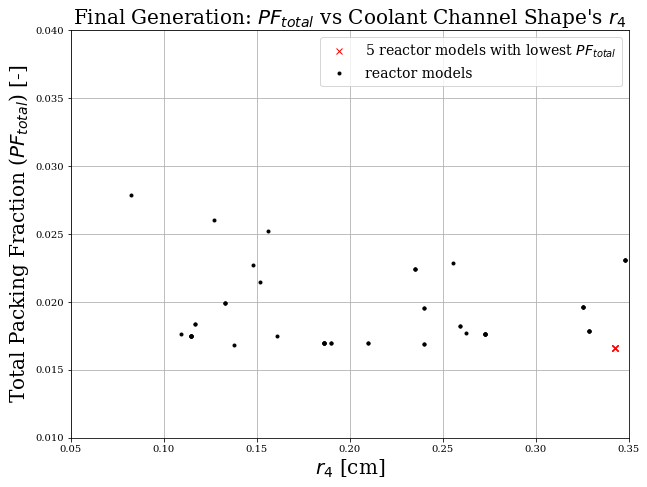
\includegraphics[width=\linewidth]{a-1d-r4.png}
        \caption{Plot of $PF_{total}$ against $r_4$.}
        \label{fig:a-1d-r4} 
    \end{subfigure}
    \begin{subfigure}{0.49\textwidth}
        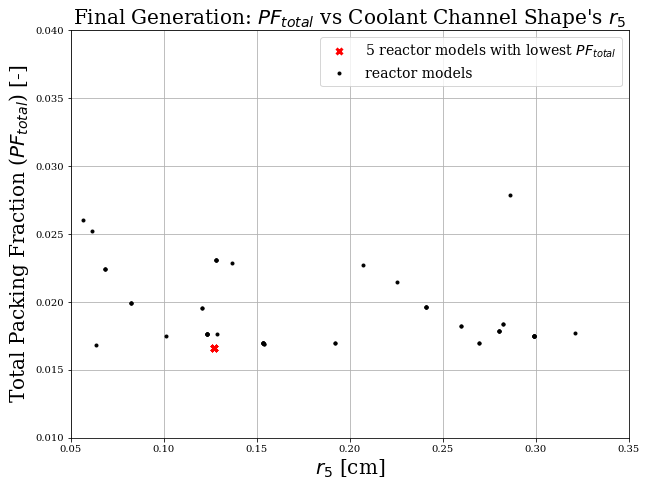
\includegraphics[width=\linewidth]{a-1d-r5.png}
        \caption{Plot of $PF_{total}$ against $r_5$.}
        \label{fig:a-1d-r5} 
    \end{subfigure}
    \caption{Simulation a-1d -- ROLLO single-objective optimization to minimize 
    total fuel packing fraction ($PF_{total}$). 
    Plots of simulation a-1d final generation's reactor models $PF_{total}$ against 
    coolant channel shape input parameters. 
    Red crosses indicate the five reactor models with the lowest $PF_{total}$.
    Input parameters varied:
    $PF_{total}$ and coolant channel shape ($r_1, r_2, r_3, r_4, r_5$).}
    \label{fig:a-1d}
\end{figure}
Figure \ref{fig:a-1d} demonstrates that there is no correlation between $PF_{total}$ 
and coolant channel shape's $r_1, r_2, r_3, r_4,$ and $r_5$. 

\subsection{Objective: Minimize Maximum Temperature ($T_{max}$)}
\label{sec:assem-1-obj-temp}
This section reports results from the minimize maximum one-third assembly temperature 
($T_{max}$) single-objective optimization simulations: a-1b and a-1e. 
Simulation a-1b varies \gls{TRISO} packing fraction distribution 
($\rho_{TRISO}(\vec{r})$), and simulation a-1e varies the coolant channel shape
($r_1, r_2, r_3, r_4,$ and $r_5$). 

\subsubsection{Simulation a-1b: Variation of $\rho_{TRISO}(\vec{r})$}
Table \ref{tab:simulationa1b} shows simulation a-1b's optimization problem parameters. 
\begin{table}[htbp!]
    \centering
    \onehalfspacing
    \caption{Simulation a-1b Optimization Problem Parameters}
	\label{tab:simulationa1b}
    \footnotesize
    \begin{tabular}{l|p{5.3cm}}
    \hline 
    \multicolumn{2}{c}{\textbf{Single Objective: Simulation a-1b}} \\
    \hline 
    \textbf{Objectives} & Minimize $T_{max}$ \\
    \hline 
    \textbf{Input Parameter variations} 
    & $\rho_{TRISO}(\vec{r})$: $0 \leq a \leq 2$, $0 \leq d \leq 2$\\
    & $\rho_{TRISO}(\vec{r})$: $0 \leq b \leq \frac{\pi}{2}$, $0 \leq e \leq \frac{\pi}{2}$\\
    & $\rho_{TRISO}(\vec{r})$: $0 \leq c \leq 2\pi$, $0 \leq f \leq 2\pi$\\
    \hline
    \textbf{Constraints} & $k_{eff} \geq 1.38$\\ 
    & $PF_{total} = 0.06 $\\ 
    \hline 
    \textbf{Genetic Algorithm Parameters} & Population size: 128 \\
    & Generations: 3 \\
    \hline
    \end{tabular}
\end{table}

Figure \ref{fig:assem-obj-1-temp-evol} shows the one-third assembly's $T_{max}$ 
evolution. 
Figure \ref{fig:assem-obj-1-temp-final} shows four unique TRISO packing fraction 
distributions in the final generation with the most minimized $T_{max}$. 
Figure \ref{fig:assem-obj-1-temp-most-minimized} illustrates the \gls{AHTR} one-third 
assembly model with the most-minimized $T_{max}$. 
\begin{figure}[htbp!]
    \begin{subfigure}{\textwidth}
        \centering
        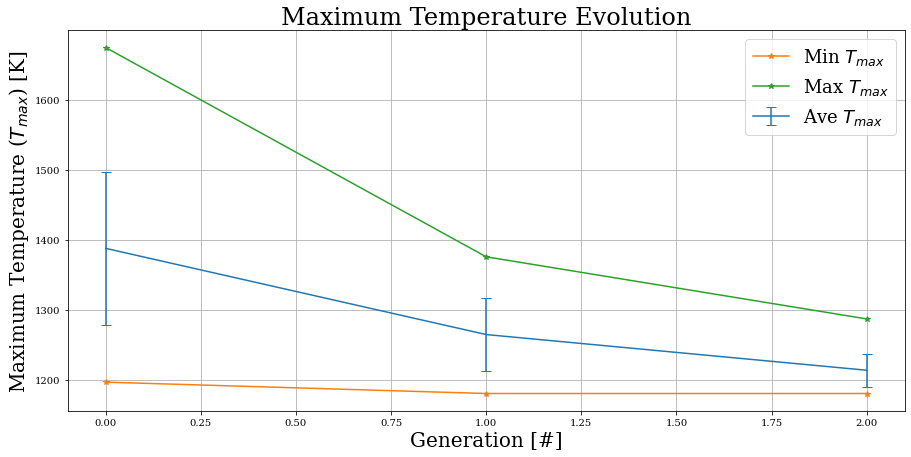
\includegraphics[width=\linewidth]{assem-obj-1-temp-evol.png}
        \caption{Minimum, average, and maximum $T_{max}$ evolution.}
        \label{fig:assem-obj-1-temp-evol} 
    \end{subfigure}
    \begin{subfigure}{\textwidth}
        \centering
        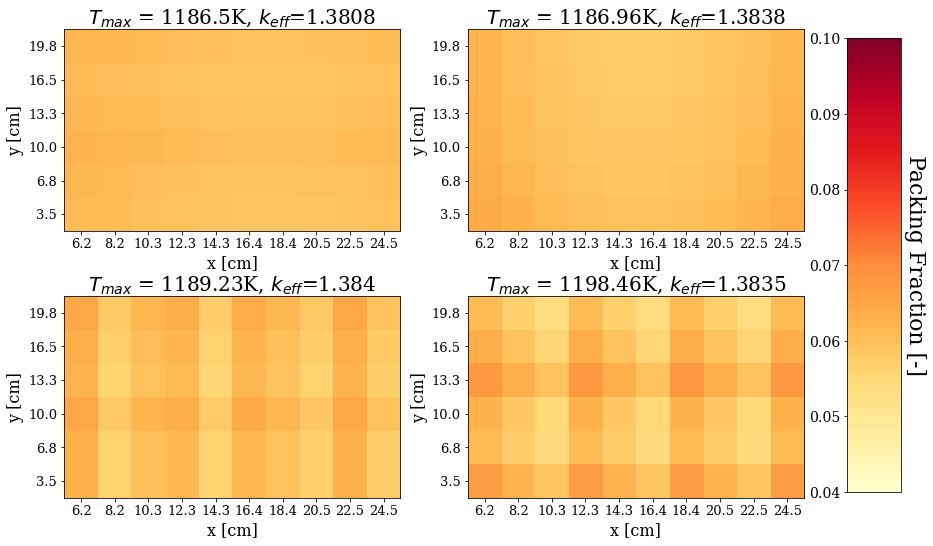
\includegraphics[width=\linewidth]{assem-obj-1-temp-final.png}
        \caption{TRISO packing fraction distribution for four unique reactor models with the 
        smallest $T_{max}$ in the final generation.}
        \label{fig:assem-obj-1-temp-final} 
    \end{subfigure}
    \caption{Simulation a-1b -- ROLLO single-objective optimization to minimize maximum 
    temperature ($T_{max}$) in the \gls{AHTR} one-third assembly. 
    Input parameters varied: \gls{TRISO} packing fraction distribution 
    ($\rho_{TRISO}(\vec{r})$).}
    \label{fig:assem-obj-1-temp}
\end{figure}
\begin{figure}[htbp!]
    \ContinuedFloat
    \begin{subfigure}{\textwidth}
        \centering
        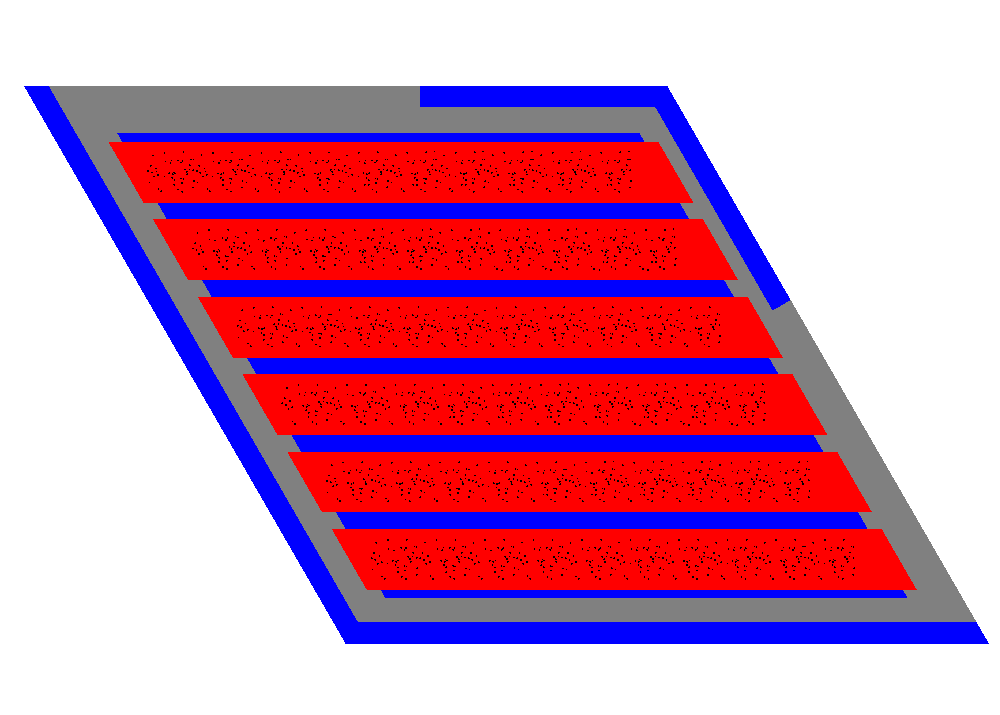
\includegraphics[width=0.7\linewidth]{assem-obj-1-temp-most-minimized.png}
        \caption{\gls{AHTR} one-third assembly model with the most-minimized 
        $T_{max}$, corresponding to the first TRISO distribution in Figure 
        \ref{fig:assem-obj-1-temp-final}. The reactor model has $T_{max}=1180.29$K
        and $k_{eff}=1.3046$.}
        \label{fig:assem-obj-1-temp-most-minimized} 
    \end{subfigure}
    \caption{Simulation a-1b -- ROLLO single-objective optimization to minimize maximum 
    temperature ($T_{max}$) in \gls{AHTR} one-third assembly. 
    Input parameters varied: \gls{TRISO} packing fraction distribution 
    ($\rho_{TRISO}(\vec{r})$).}
\end{figure}

Figure \ref{fig:assem-obj-1-temp-evol} shows that the minimum and average one-third 
assembly's $T_{max}$ converged to approximately 1200 K.
In Figure \ref{fig:assem-obj-1-temp-final}, the one-third assembly model with the 
most-minimized $T_{max}$ has a $T_{max}=1186.5$K and an almost constant TRISO packing 
fraction distribution with packing fraction standard deviation of $0.0009$ across the 
one-third assembly. 
Section \ref{sec:assem-discussion-temp} discusses and explains simulation a-1b's 
most-minimized $T_{max}$ almost constant TRISO distribution. 

\subsubsection{Simulation a-1e: Variation of Coolant channel shape}
Table \ref{tab:simulationa1e} shows simulation a-1e's optimization problem parameters. 
\begin{table}[htbp!]
    \centering
    \onehalfspacing
    \caption{Simulation a-1e Optimization Problem Parameters}
	\label{tab:simulationa1e}
    \footnotesize
    \begin{tabular}{l|p{6cm}}
    \hline 
    \multicolumn{2}{c}{\textbf{Single Objective: Simulation a-1e}} \\
    \hline 
    \textbf{Objectives} & Minimize $T_{max}$ \\
    \hline 
    \textbf{Input Parameter variations} 
    & coolant channel shape: $0.05<r_{1}<0.35$ \\
    & coolant channel shape: $0.05<r_{2}<0.35$ \\
    & coolant channel shape: $0.05<r_{3}<0.35$ \\
    & coolant channel shape: $0.05<r_{4}<0.35$ \\
    & coolant channel shape: $0.05<r_{5}<0.35$ \\
    \hline
    \textbf{Constraints} & $k_{eff} \geq 1.38$\\ 
    & $PF_{total} = 0.06 $\\ 
    \hline 
    \textbf{Genetic Algorithm Parameters} & Population size: 128 \\
    & Generations: 2 \\
    \hline
    \end{tabular}
\end{table}

Figure \ref{fig:a-1e-evol} shows the one-third assembly's $T_{max}$ evolution.
Figure \ref{fig:assem-obj-1-temp-most-minimized-coolant} illustrates the \gls{AHTR} 
one-third assembly model with the most-minimized $T_{max}$. 
Figures \ref{fig:a-1e-r1}, \ref{fig:a-1e-r2}, \ref{fig:a-1e-r3}, \ref{fig:a-1e-r4}, 
and \ref{fig:a-1e-r5} show the plots of coolant channel shape's 
$r_1, r_2, r_3, r_4,$ and $r_5$ values against $T_{max}$. 
\begin{figure}[htbp!]
    \begin{subfigure}{\textwidth}
        \centering
        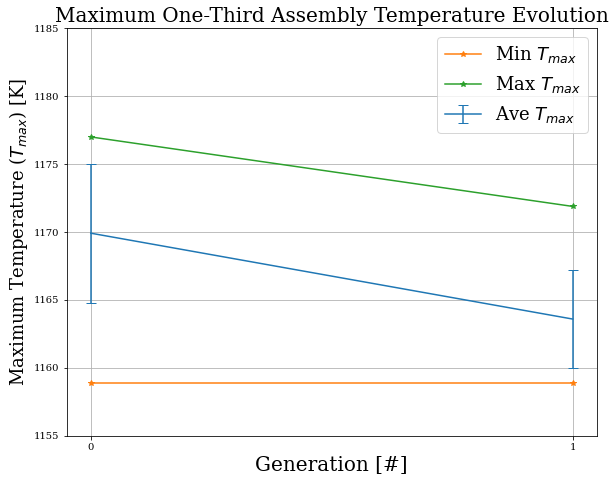
\includegraphics[width=\linewidth]{a-1e-evol.png}
        \caption{Minimum, average, and maximum evolution of AHTR one-third assembly's 
        $T_{max}$.}
        \label{fig:a-1e-evol} 
    \end{subfigure}
    \begin{subfigure}{\textwidth}
        \centering
        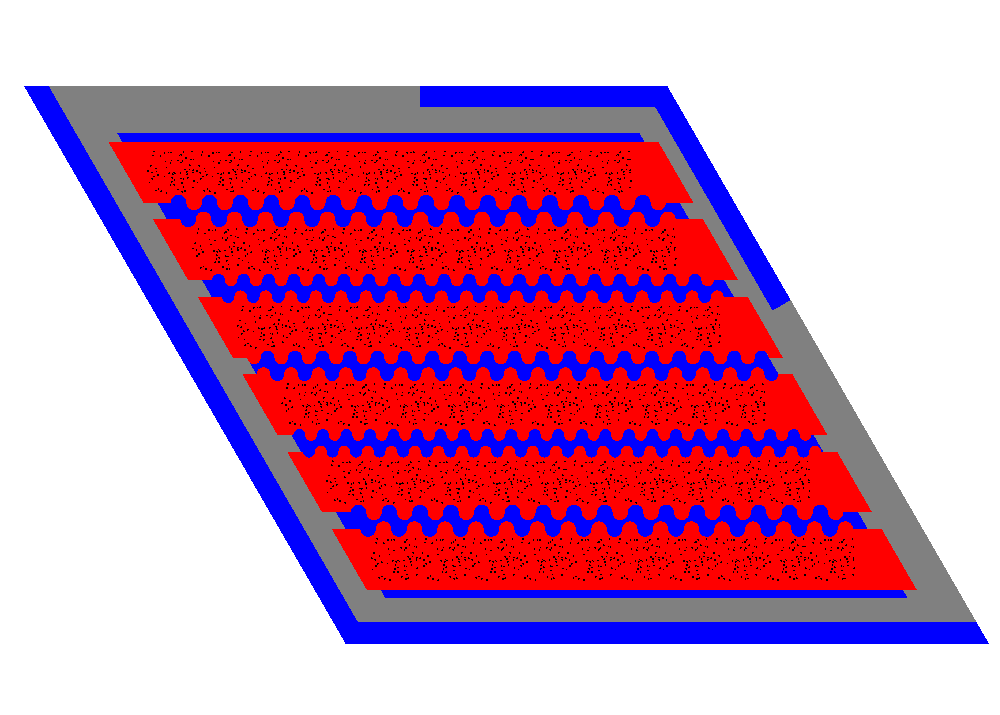
\includegraphics[width=0.8\linewidth]{assem-obj-1-temp-most-minimized-coolant.png}
        \caption{\gls{AHTR} one-third assembly model with the most-minimized $T_{max}$. 
        The reactor model has $T_{max} = 1161.28K$, $r_1 = 0.32cm$, $r_{2} = 0.26cm$,
        $r_3 = 0.28cm$, $r_{4} = 0.24cm$, and $r_{5} = 0.32cm$.}
        \label{fig:assem-obj-1-temp-most-minimized-coolant} 
    \end{subfigure}
    \caption{Simulation a-1e -- ROLLO single-objective optimization to minimize 
    maximum one-third assembly temperature ($T_{max}$). 
    Plots of final generation's reactor models $T_{max}$ against 
    coolant channel shape input parameters. 
    Red crosses indicate the five reactor models with the lowest $T_{max}$.
    Input parameters varied: coolant channel shape ($r_1, r_2, r_3, r_4, r_5$).}
    \label{fig:a-1e}
\end{figure}
\begin{figure}[htbp!]
    \ContinuedFloat
    \centering
    \begin{subfigure}{0.49\textwidth}
        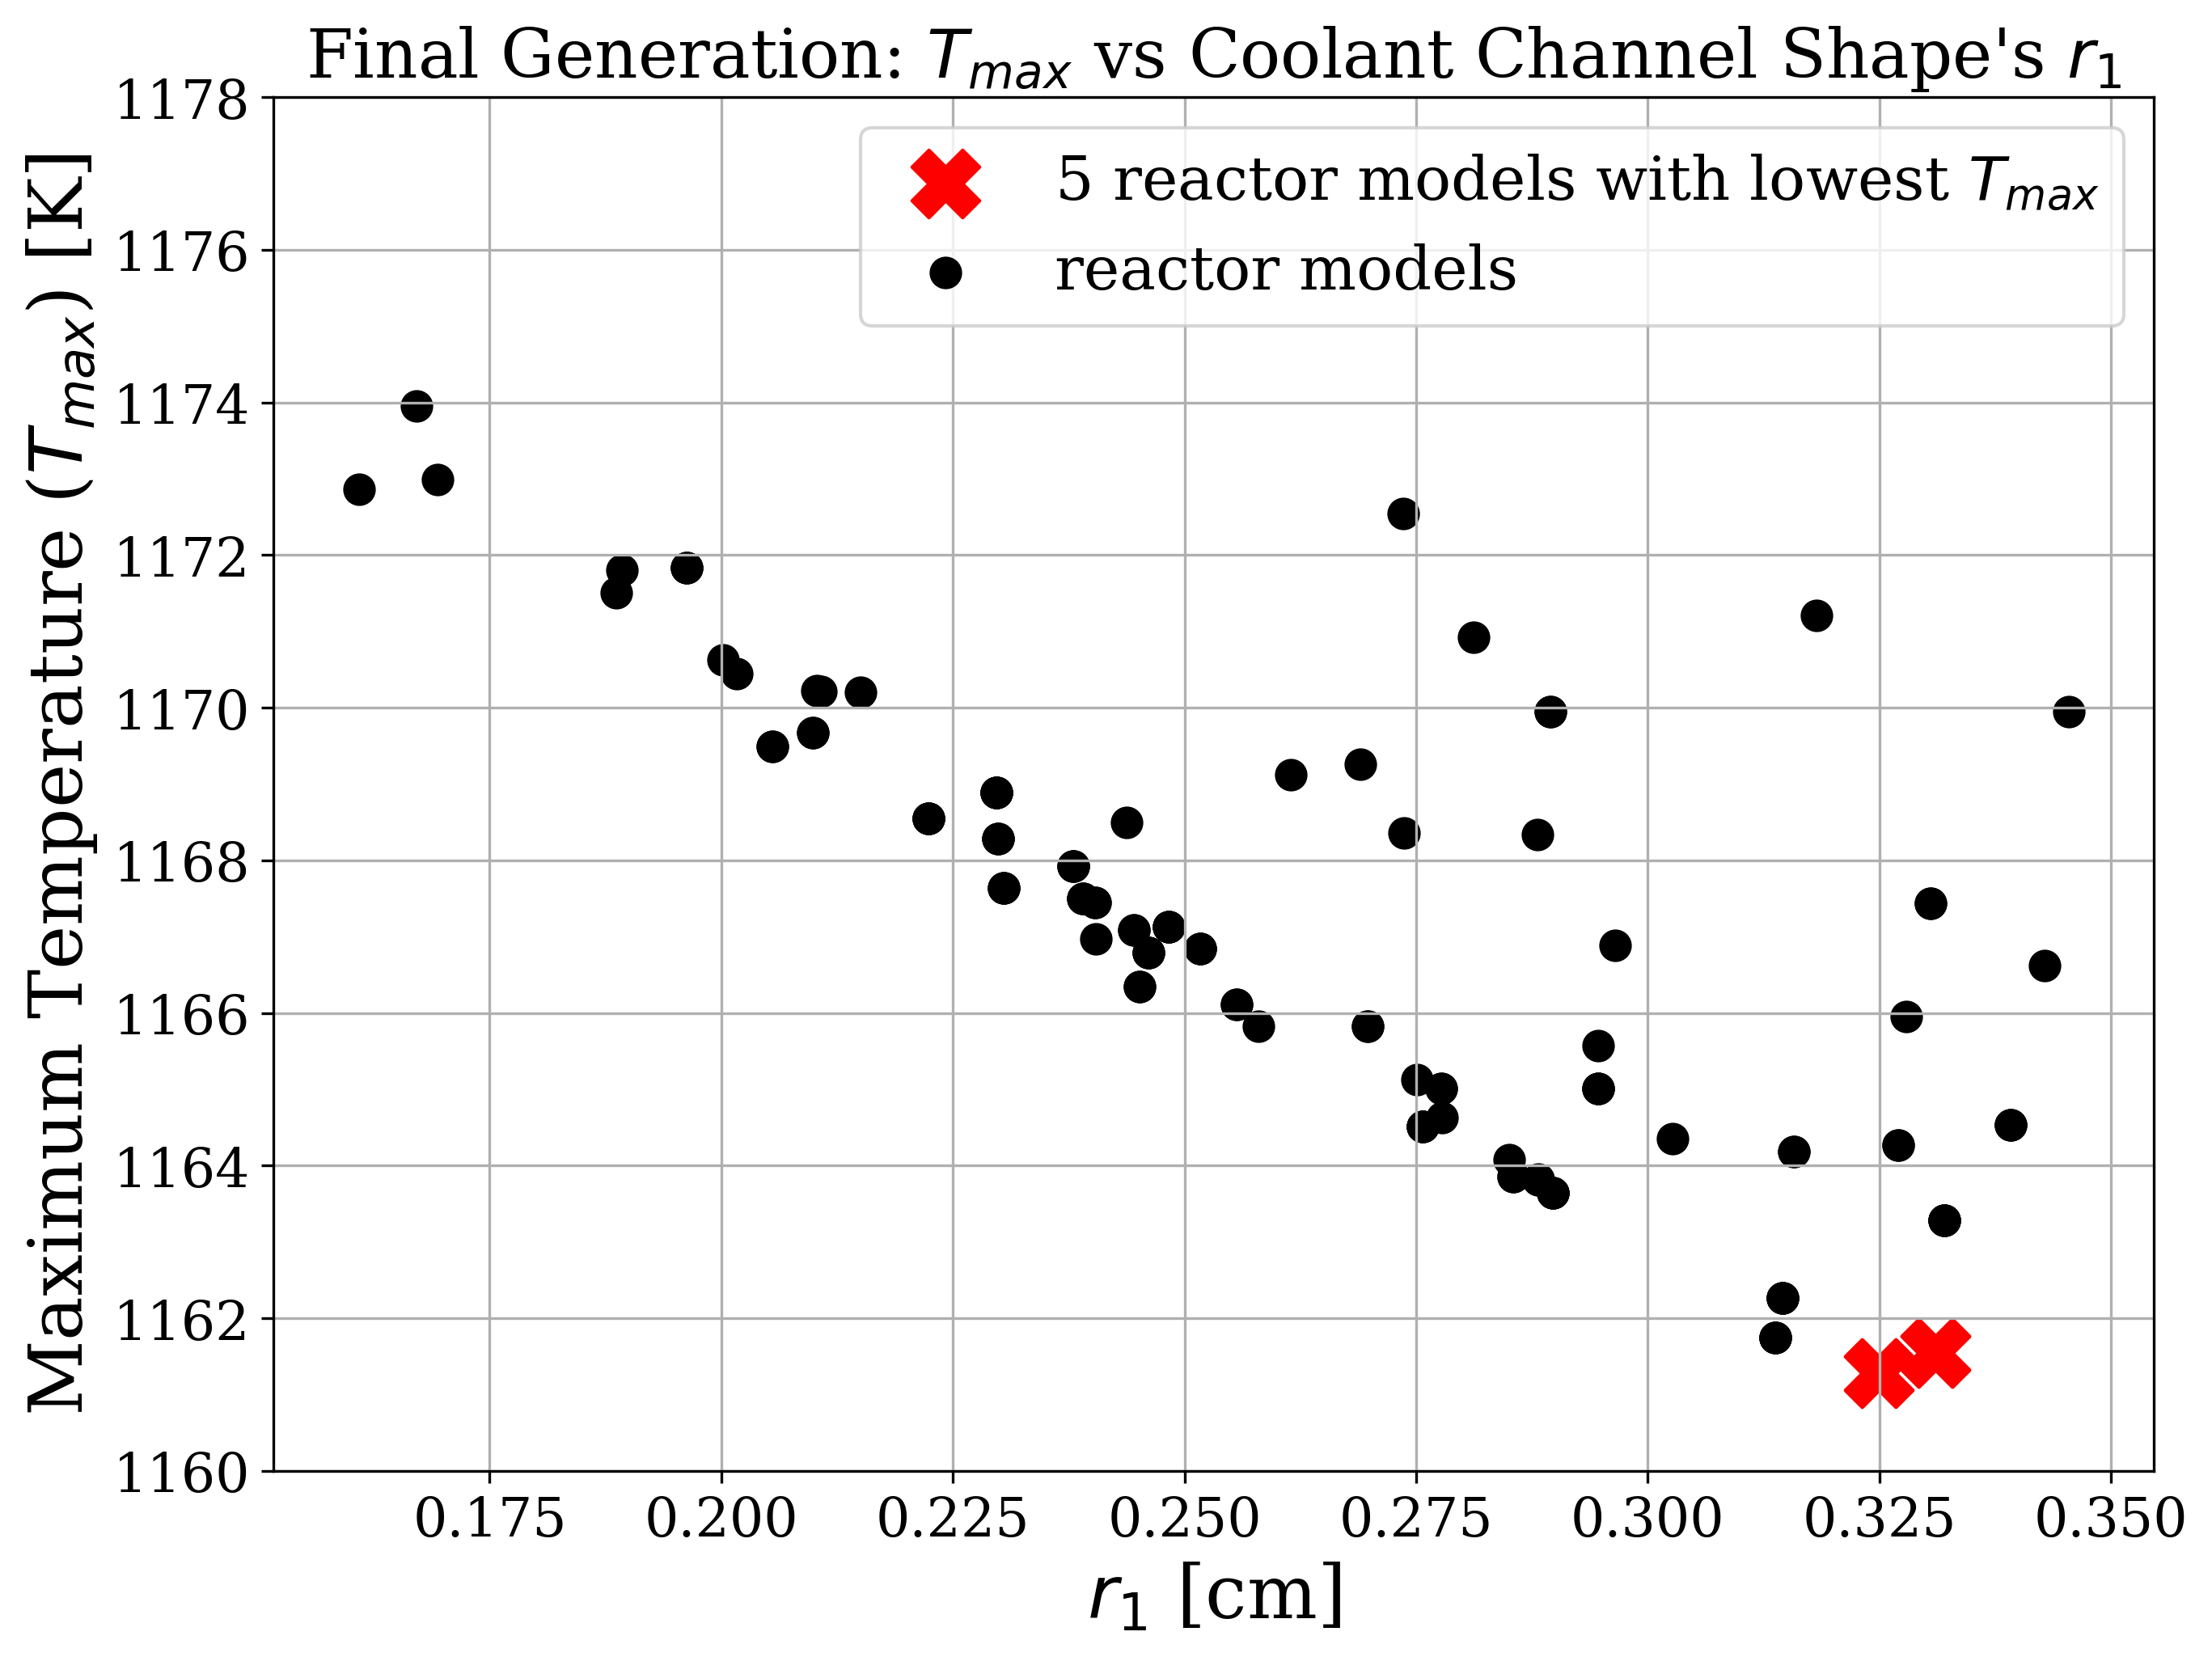
\includegraphics[width=\linewidth]{a-1e-r1.png}
        \caption{Plot of $PF_{total}$ against $r_1$.}
        \label{fig:a-1e-r1} 
    \end{subfigure}
    \begin{subfigure}{0.49\textwidth}
        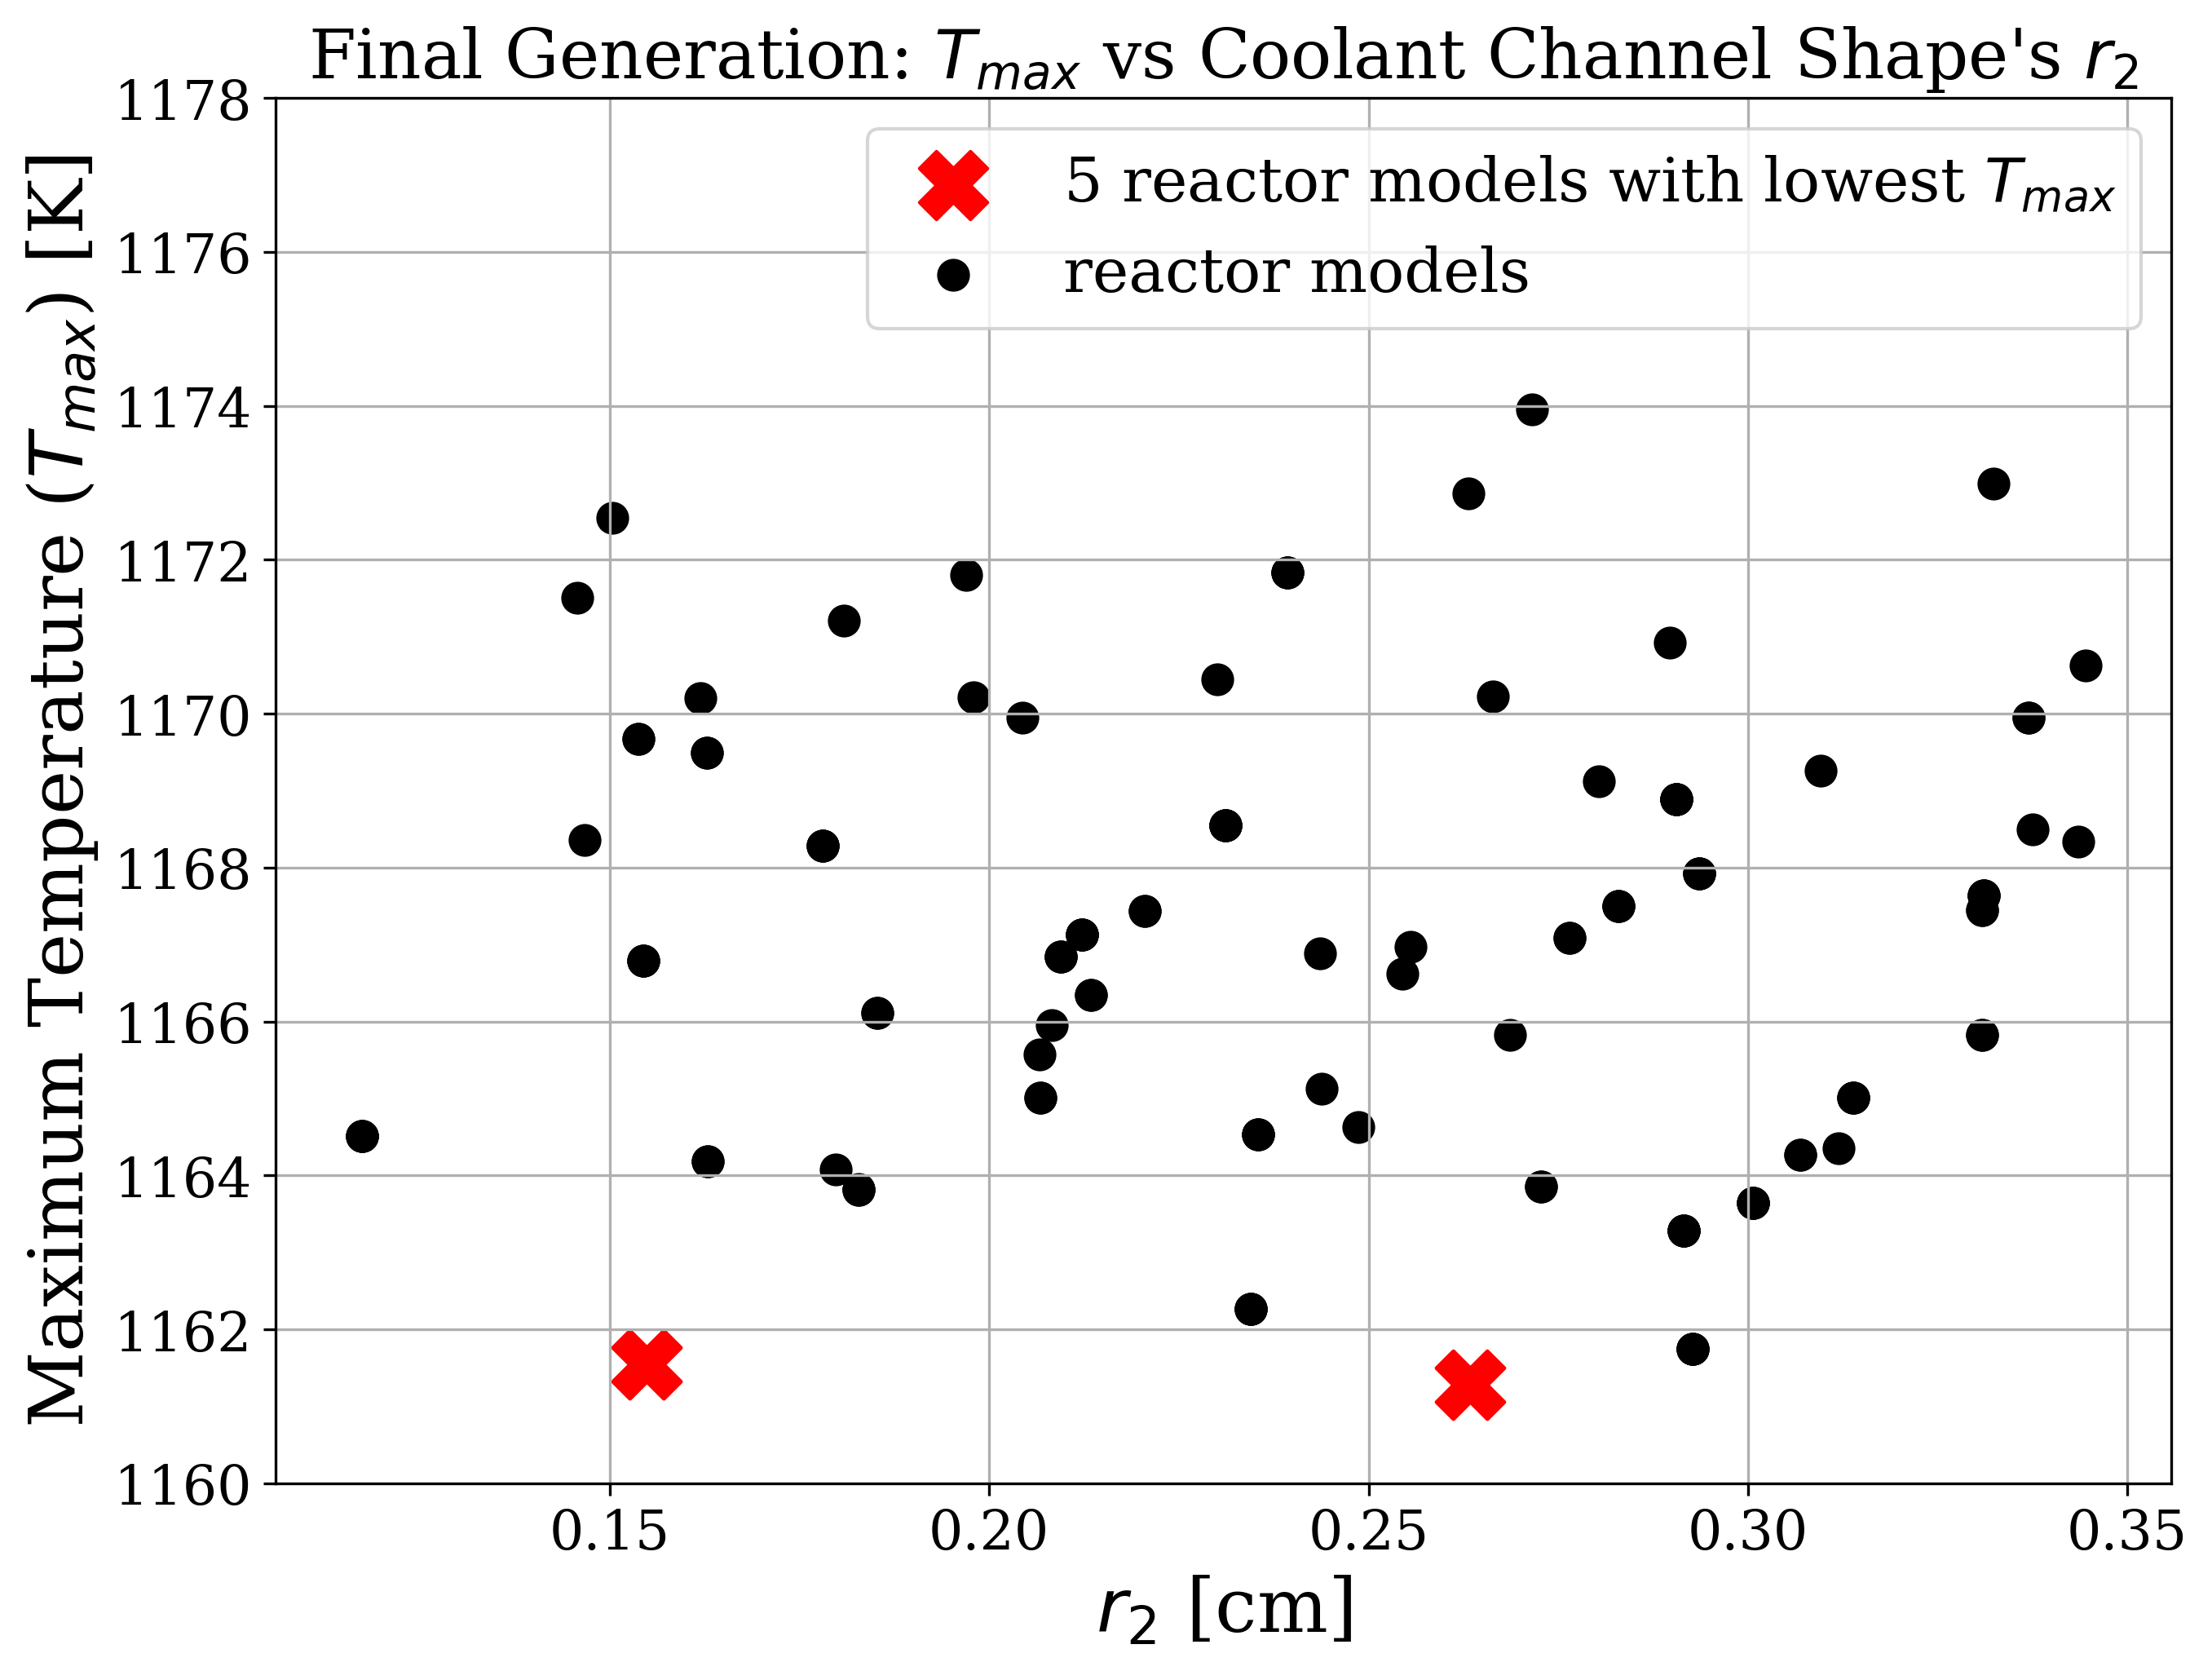
\includegraphics[width=\linewidth]{a-1e-r2.png}
        \caption{Plot of $PF_{total}$ against $r_2$.}
        \label{fig:a-1e-r2} 
    \end{subfigure}
    \begin{subfigure}{0.49\textwidth}
        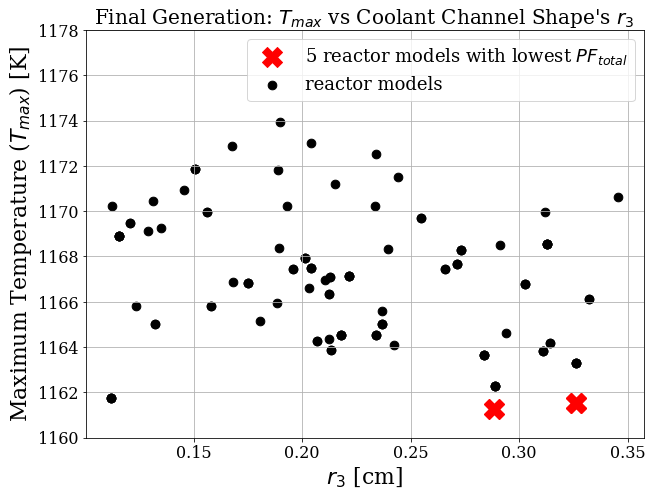
\includegraphics[width=\linewidth]{a-1e-r3.png}
        \caption{Plot of $PF_{total}$ against $r_3$.}
        \label{fig:a-1e-r3} 
    \end{subfigure}
    \begin{subfigure}{0.49\textwidth}
        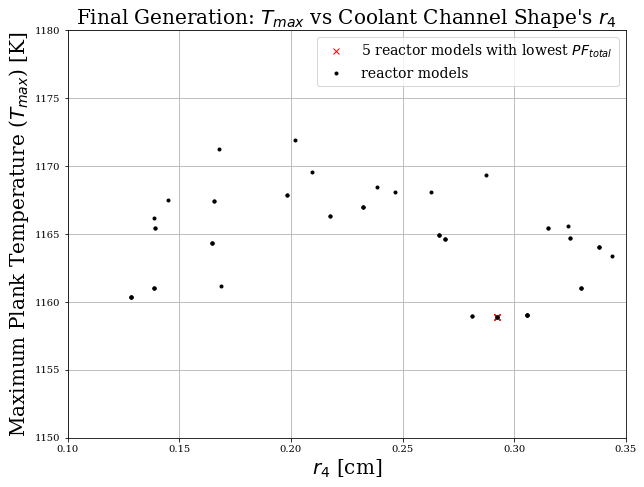
\includegraphics[width=\linewidth]{a-1e-r4.png}
        \caption{Plot of $PF_{total}$ against $r_4$.}
        \label{fig:a-1e-r4} 
    \end{subfigure}
    \begin{subfigure}{0.49\textwidth}
        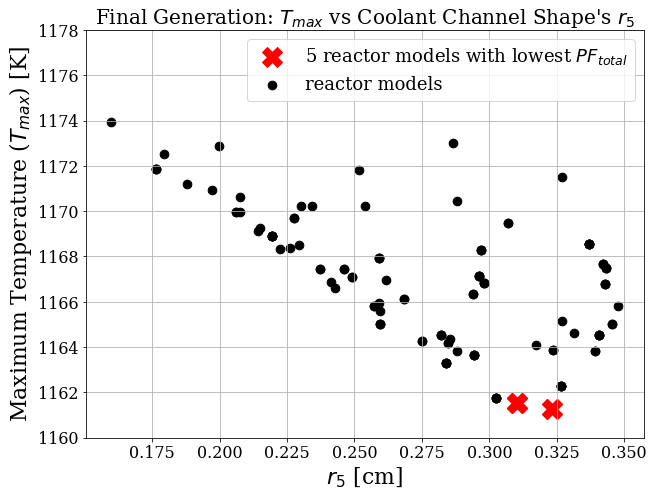
\includegraphics[width=\linewidth]{a-1e-r5.png}
        \caption{Plot of $PF_{total}$ against $r_5$.}
        \label{fig:a-1e-r5} 
    \end{subfigure}
    \caption{Simulation a-1e -- ROLLO single-objective optimization to minimize 
    maximum one-third assembly temperature ($T_{max}$). 
    Plots of final generation's reactor models $T_{max}$ against 
    coolant channel shape input parameters. 
    Red crosses indicate the five reactor models with the lowest $T_{max}$.
    Input parameters varied: coolant channel shape ($r_1, r_2, r_3, r_4, r_5$).}
\end{figure}

Figures \ref{fig:a-1e-r1} and \ref{fig:a-1e-r5} demonstrate negative linear correlations 
between the one-third assembly's $T_{max}$ with $r_1$ and $r_5$. 
Figures \ref{fig:a-1e-r2}, \ref{fig:a-1e-r3} and \ref{fig:a-1e-r4} demonstrate that 
there is no correlation between $T_{max}$ with $r_2$, $r_3$, and $r_4$. 
Section \ref{sec:assem-discussion-temp} discusses and explains the relationship between 
$T_{max}$ and coolant channel shape. 

\subsection{Objective: Minimize Fuel-Normalized Power Peaking Factor ($PPF_{fuel}$)}
\label{sec:assem-1-obj-ppf}
This section reports the minimize fuel-normalized power peaking factor 
($PPF_{fuel}$) single-objective optimization simulation results: a-1c and a-1f. 
Simulation a-1c varies \gls{TRISO} packing fraction distribution 
($\rho_{TRISO}(\vec{r})$), and simulation a-1f varies the coolant channel shape 
($r_1, r_2, r_3, r_4,$ and $r_5$).

\subsubsection{Simulation a-1c: Variation of $\rho_{TRISO}(\vec{r})$}
Table \ref{tab:simulationa1c} shows simulation a-1c's optimization problem parameters. 
\begin{table}[htbp!]
    \centering
    \onehalfspacing
    \caption{Simulation a-1c Optimization Problem Parameters}
	\label{tab:simulationa1c}
    \footnotesize
    \begin{tabular}{l|p{5.3cm}}
    \hline 
    \multicolumn{2}{c}{\textbf{Single Objective: Simulation a-1c}} \\
    \hline 
    \textbf{Objectives} & Minimize $PPF_{fuel}$ \\
    \hline 
    \textbf{Input Parameter variations}
    & $\rho_{TRISO}(\vec{r})$: $0 \leq a \leq 2$, $0 \leq d \leq 2$\\
    & $\rho_{TRISO}(\vec{r})$: $0 \leq b \leq \frac{\pi}{2}$, $0 \leq e \leq \frac{\pi}{2}$\\
    & $\rho_{TRISO}(\vec{r})$: $0 \leq c \leq 2\pi$, $0 \leq f \leq 2\pi$\\
    \hline
    \textbf{Constraints} & $k_{eff} \geq 1.38$\\ 
    & $PF_{total}$ = 0.06 \\
    \hline 
    \textbf{Genetic Algorithm Parameters} & Population size: 128 \\
    & Generations: 2 \\
    \hline
    \end{tabular}
\end{table}

Figure \ref{fig:assem-obj-1-ppf-evol} shows the one-third assembly's $PPF_{fuel}$ 
evolution. 
Figure \ref{fig:assem-obj-1-ppf-final} shows the four unique TRISO packing fraction 
distributions in the final generation with the most minimized $PPF_{fuel}$. 
Figure \ref{fig:assem-obj-1-ppf-most-minimized} illustrates the \gls{AHTR} one-third 
assembly model with the most-minimized $PPF_{fuel}$. 
\begin{figure}[htbp!]
    \begin{subfigure}{\textwidth}
        \centering
        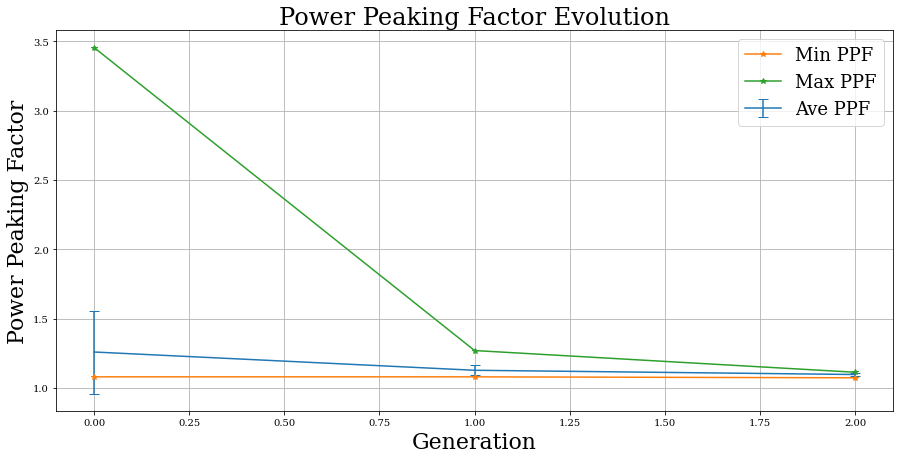
\includegraphics[width=\linewidth]{assem-obj-1-ppf-evol.png}
        \caption{Minimum, average, and maximum evolution of $PPF_{fuel}$ in the 
        AHTR one-third assembly.}
        \label{fig:assem-obj-1-ppf-evol} 
    \end{subfigure}
    \begin{subfigure}{\textwidth}
        \centering
        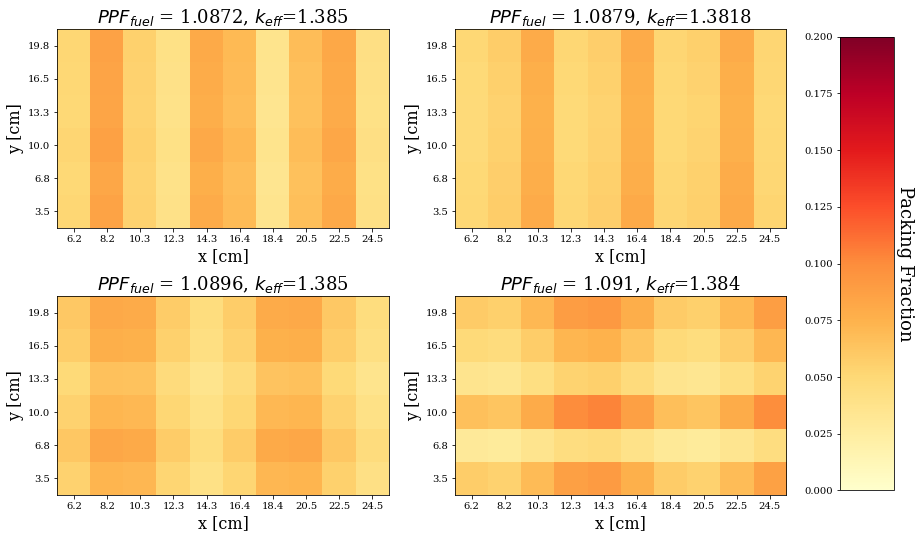
\includegraphics[width=\linewidth]{assem-obj-1-ppf-final.png}
        \caption{TRISO distribution for the four unique reactor models with the 
        lowest $PPF_{fuel}$ in the AHTR one-third assembly at the final generation.}
        \label{fig:assem-obj-1-ppf-final} 
    \end{subfigure}
    \caption{Simulation a-1c -- ROLLO single-objective optimization to minimize 
    AHTR one-third assembly's fuel-normalized power peaking factor ($PPF_{fuel}$). 
    Input parameters varied: TRISO distribution ($\rho_{TRISO}(\vec{r})$).
    $PF_{total}$ = 0.06.}
    \label{fig:assem-obj-1-ppf}
\end{figure}
\begin{figure}[htbp!]
    \ContinuedFloat
    \begin{subfigure}{\textwidth}
        \centering
        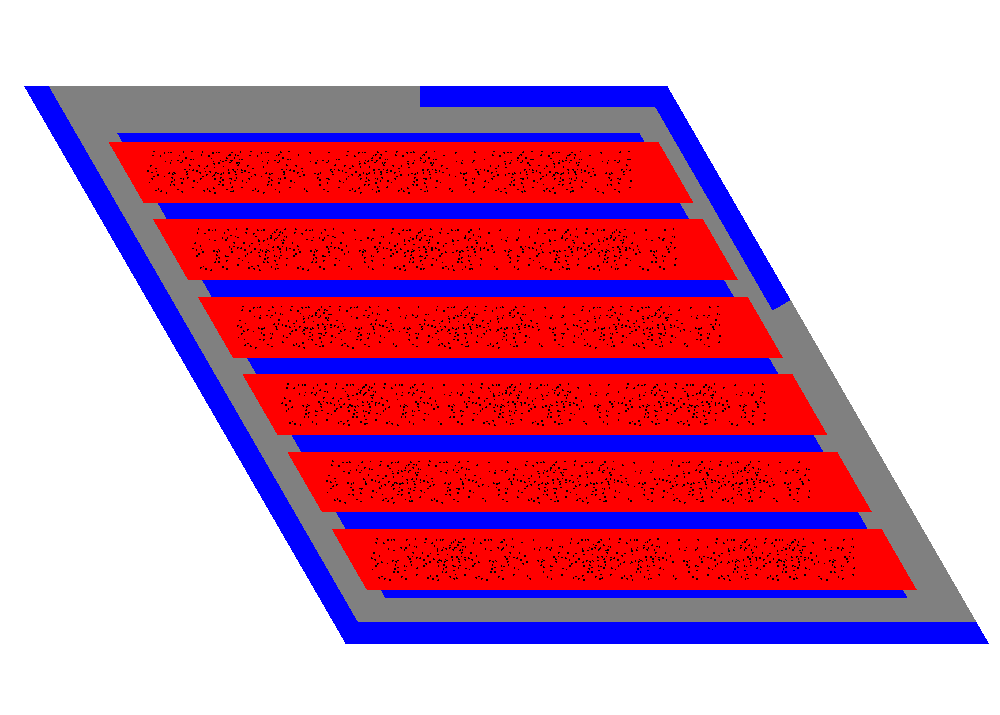
\includegraphics[width=0.7\linewidth]{assem-obj-1-ppf-most-minimized.png}
        \caption{\gls{AHTR} one-third assembly model with the most-minimized 
        $PPF_{fuel}$, corresponding to the first TRISO distribution in Figure 
        \ref{fig:assem-obj-1-ppf-final}. The reactor model has $PPF_{fuel}=1.0872$
        and $k_{eff}=1.385$.}
        \label{fig:assem-obj-1-ppf-most-minimized} 
    \end{subfigure}
    \caption{Simulation a-1c -- ROLLO single-objective optimization to minimize 
    AHTR one-third assembly's fuel-normalized power peaking factor ($PPF_{fuel}$). 
    Input parameters varied: TRISO distribution ($\rho_{TRISO}(\vec{r})$).
    $PF_{total}$ = 0.06.}
\end{figure}

Figure \ref{fig:assem-obj-1-ppf-evol} shows that the minimum and average 
one-third assembly's $T_{max}$ converged to approximately 1.1.
In Figure \ref{fig:assem-obj-1-ppf-final}, the most-minimized TRISO distribution has 
a $PPF_{fuel} = 1.0872$ and an oscillating TRISO distribution along the x-axis and a 
packing fraction standard deviation of $0.017$ across the one-third assembly. 
Along the x-axis, the distribution peaks at the 2nd, 5th, and 9th fuel 
cell columns (at 8.2cm, 14.3cm, and 22.5cm) with $PF\approx0.08$ and has minimum points
at the 4th and 7th fuel cell columns (at 12.3cm and 18.4cm) with $PF\approx0.035$. 
Section \ref{sec:assem-discussion-ppf} discusses the driving factors for the minimize 
$PPF_{fuel}$ objective and explains simulation a-1c's most-minimized $PPF_{fuel}$ 
TRISO distribution. 

\subsubsection{Simulation a-1f: Variation of Coolant channel shape}
Table \ref{tab:simulationa1f} shows simulation a-1f's optimization problem parameters. 
\begin{table}[htbp!]
    \centering
    \onehalfspacing
    \caption{Simulation a-1f Optimization Problem Parameters}
	\label{tab:simulationa1f}
    \footnotesize
    \begin{tabular}{l|p{6cm}}
    \hline 
    \multicolumn{2}{c}{\textbf{Single Objective: Simulation a-1f}} \\
    \hline 
    \textbf{Objectives} & Minimize $PPF_{fuel}$ \\
    \hline 
    \textbf{Input Parameter variations} 
    & coolant channel shape: $0.05<r_{1}<0.35$ \\
    & coolant channel shape: $0.05<r_{2}<0.35$ \\
    & coolant channel shape: $0.05<r_{3}<0.35$ \\
    & coolant channel shape: $0.05<r_{4}<0.35$ \\
    & coolant channel shape: $0.05<r_{5}<0.35$ \\
    \hline
    \textbf{Constraints} & $k_{eff} \geq 1.0$\\ 
    & $PF_{total}$ = 0.04 \\
    \hline 
    \textbf{Genetic Algorithm Parameters} & Population size: 64 \\
    & Generations: 2 \\
    \hline
    \end{tabular}
\end{table}

Figure \ref{fig:a-1f} shows the plots of coolant channel shape's 
$r_1, r_2, r_3, r_4,$ and $r_5$ values against $PPF_{fuel}$. 
\begin{figure}[htbp!]
    \centering
    \begin{subfigure}{0.49\textwidth}
        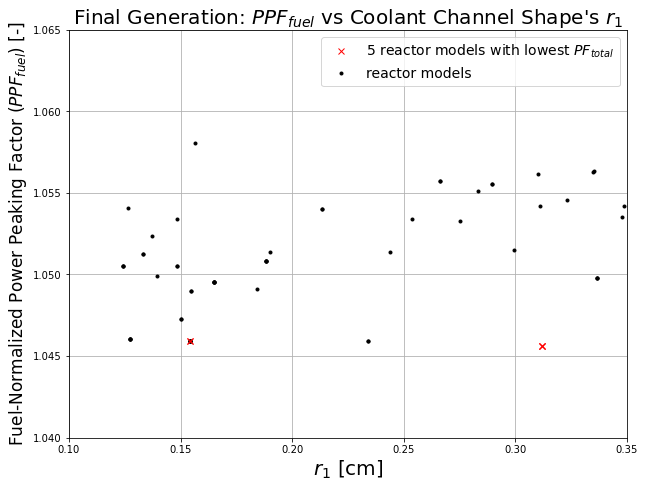
\includegraphics[width=\linewidth]{a-1f-r1.png}
        \caption{Plot of $PF_{total}$ against $r_1$.}
        \label{fig:a-1f-r1} 
    \end{subfigure}
    \begin{subfigure}{0.49\textwidth}
        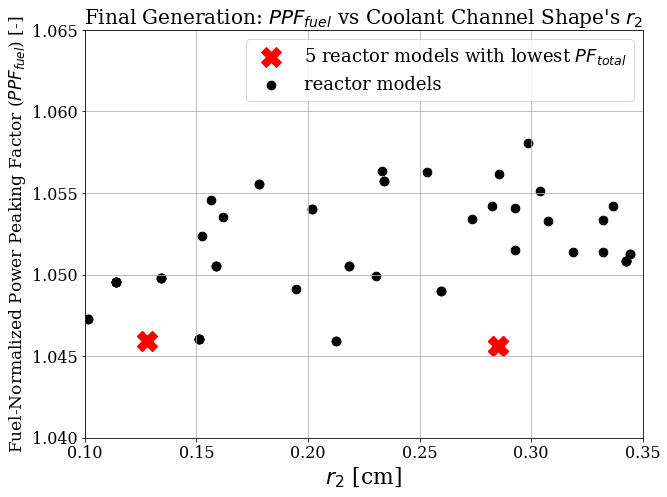
\includegraphics[width=\linewidth]{a-1f-r2.png}
        \caption{Plot of $PF_{total}$ against $r_2$.}
        \label{fig:a-1f-r2} 
    \end{subfigure}
    \begin{subfigure}{0.49\textwidth}
        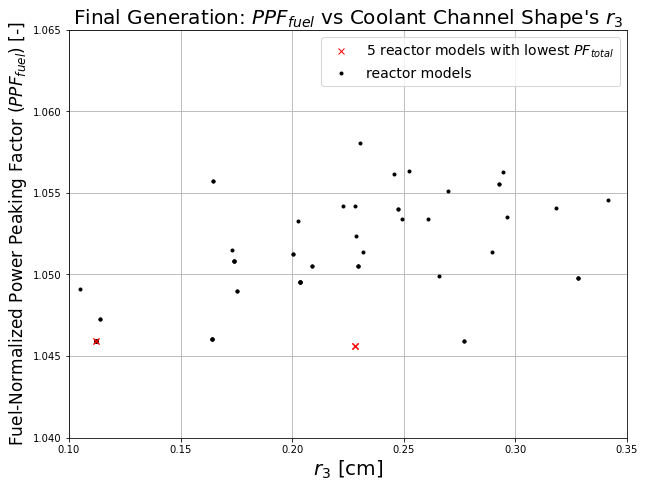
\includegraphics[width=\linewidth]{a-1f-r3.png}
        \caption{Plot of $PF_{total}$ against $r_3$.}
        \label{fig:a-1f-r3} 
    \end{subfigure}
    \begin{subfigure}{0.49\textwidth}
        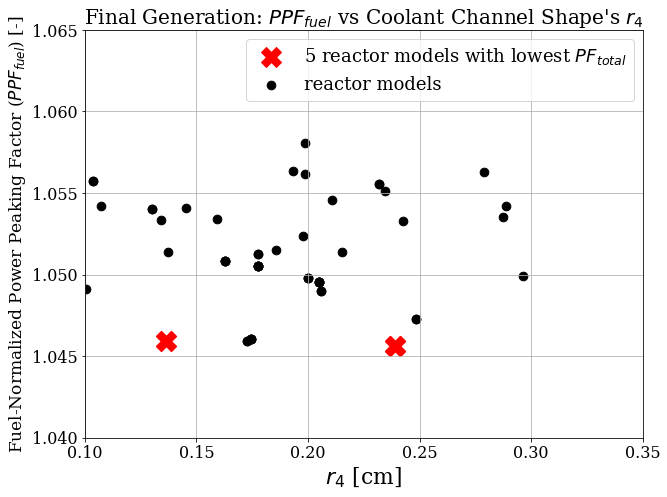
\includegraphics[width=\linewidth]{a-1f-r4.png}
        \caption{Plot of $PF_{total}$ against $r_4$.}
        \label{fig:a-1f-r4} 
    \end{subfigure}
    \begin{subfigure}{0.49\textwidth}
        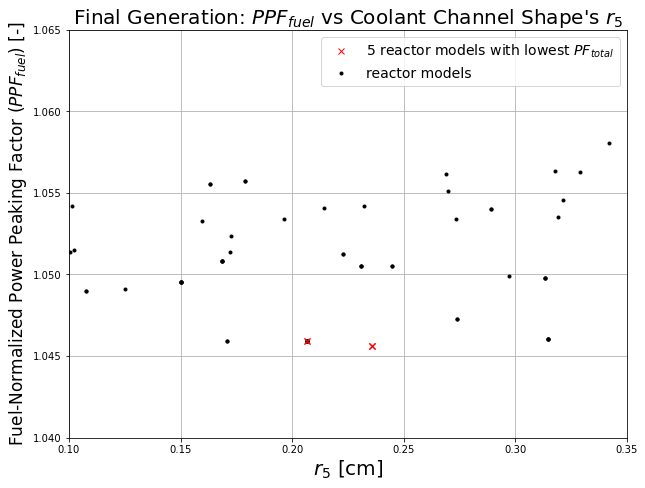
\includegraphics[width=\linewidth]{a-1f-r5.png}
        \caption{Plot of $PF_{total}$ against $r_5$.}
        \label{fig:a-1f-r5} 
    \end{subfigure}
    \caption{Simulation a-1f -- ROLLO single-objective optimization to minimize 
    AHTR one-third assembly's fuel-normalized power peaking factor ($PPF_{fuel}$). 
    Plots of simulation a-1f final generation's reactor models $PPF_{fuel}$ against 
    coolant channel shape input parameters. 
    Red crosses indicate the five reactor models with the lowest $PPF_{fuel}$.
    Input parameters varied: total fuel packing fraction 
    ($PPF_{fuel}$), and coolant channel shape ($r_1, r_2, r_3, r_4, r_5$).}
    \label{fig:a-1f}
\end{figure}
Figure \ref{fig:a-1f} demonstrates that there is no correlation between $PPF_{fuel}$ 
and coolant channel shape's $r_1, r_2, r_3, r_4,$ and $r_5$. 

\section{AHTR One-Third Assembly: Two-Objective Optimization Results}
\label{sec:assem-two-obj}
This section reports the \gls{AHTR} one-third assembly's \gls{ROLLO} two-objective 
optimization results. 
The previous section's one-objective optimization results inform the multi-objective 
optimization simulations in this section and Section \ref{sec:assem-three-obj}.
Since the variations in coolant channel shape only impact one objective: 
minimize one-third assembly's maximum temperature ($T_{max}$), I do not conduct 
two-objective optimization for coolant channel shape variations.  
Table \ref{tab:assem-obj-breakdown} summarized the two-objective simulations: 
a-2a, a-2b, and a-2c.

As described in Section \ref{sec:opt}, multi-objective optimization returns 
multiple optimal solutions that meet each objective to varying degrees; this set of 
solutions is the Pareto front \cite{deb_multi-objective_2001}. 
For each solution in the Pareto front, none of the objective functions can be 
improved without degrading another objective.
An ideal optimization method for a multi-objective problem like reactor design 
optimization should find widely spread out reactor model solutions in the Pareto front 
\cite{deb_multi-objective_2001}. 
Thus, I report on the optimal reactor models on the Pareto front for the multi-objective 
optimization problems in this section and Section \ref{sec:assem-three-obj}. 

To ensure that the multi-objective optimization problems are converged, I report the 
hypervolume values for each generation. 
As previously described in Section \ref{sec:binhandkorn}, the hypervolume indicator 
quantifies the Pareto front's goodness (bigger = better).
I use a different reference point for each optimization problem. 
If a multi-objective optimization problem's hypervolume converges earlier than the 
five generations I intended to run (determined in Section 
\ref{sec:multi-obj-hyperparameters}), I stop the simulation at that generation. 

\subsection{a-2a: Minimize $PF_{total}$ and $T_{max}$}
\label{sec:a-2a}
This section reports results from the two-objective optimization simulation a-2a;
minimized objectives are total fuel packing fraction ($PF_{total}$) and maximum 
temperature ($T_{max}$) in the one-third assembly.  
Table \ref{tab:simulationa2a} shows simulation a-2a's optimization problem parameters. 
\begin{table}[htbp!]
    \centering
    \onehalfspacing
    \caption{Simulation a-2a Optimization Problem Parameters}
	\label{tab:simulationa2a}
    \footnotesize
    \begin{tabular}{l|p{5.3cm}}
    \hline 
    \multicolumn{2}{c}{\textbf{Two Objectives: Simulation a-2a}} \\
    \hline 
    \textbf{Objectives} & Minimize $PF_{total}$ \\
    & Minimize $T_{max}$ \\
    \hline 
    \textbf{Input parameter variations} & $0.05 \leq PF_{total} \leq 0.07$ \\
    & $\rho_{TRISO}(\vec{r})$: $0 \leq a \leq 2$, $0 \leq d \leq 2$\\
    & $\rho_{TRISO}(\vec{r})$: $0 \leq b \leq \frac{\pi}{2}$, $0 \leq e \leq \frac{\pi}{2}$\\
    & $\rho_{TRISO}(\vec{r})$: $0 \leq c \leq 2\pi$, $0 \leq f \leq 2\pi$\\
    \hline
    \textbf{Constraints} & $k_{eff} \geq 1.38$\\ 
    \hline 
    \textbf{Genetic algorithm parameters} & Population size: 128 \\
    & Generations: 5 \\
    \hline
    \end{tabular}
\end{table}

Table \ref{tab:a2a-hypervolume} shows the hypervolume value at each generation, 
confirming that simulation a-2a converges by generation 5. 
\begin{table}[htbp!]
    \centering
    \onehalfspacing
    \caption{Simulation a-2a hypervolume values at each generation.}
	\label{tab:a2a-hypervolume}
    \footnotesize
    \begin{tabular}{ll}
    \hline 
    \multicolumn{2}{c}{\textbf{Two Objectives: Simulation a-2a}} \\
    \multicolumn{2}{c}{Reference point: (0.07, 1700)} \\
    \hline 
    \textbf{Generation} & \textbf{Hypervolume [-]} \\
    \hline
    1 & 6.0090 \\
    2 & 6.0859 \\
    3 & 6.2220 \\
    4 & 6.3379 \\
    5 & 6.4664 \\
    \hline
    \end{tabular}
\end{table}

Figure \ref{fig:assem-obj-2-pftemp-pareto} shows a plot of the final generation's reactor 
models' $PF_{total}$ against $T_{max}$; crosses mark the reactor models that fall on 
the Pareto front.
Figure \ref{fig:assem-obj-2-pftemp-pareto-distr} shows the 22 TRISO packing fraction 
distributions in the final generation that fall on the Pareto front. 
\begin{figure}[htbp!]
    \begin{subfigure}{\textwidth}
        \centering
        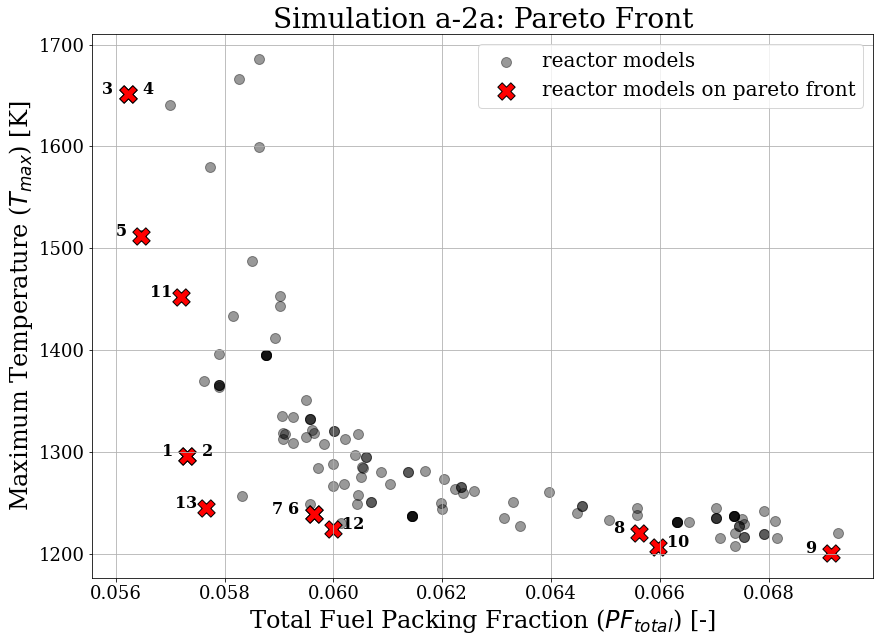
\includegraphics[width=\linewidth]{assem-obj-2-pftemp-pareto.png}
        \caption{Plot of final generation's reactor models' $PF_{total}$ against 
        $T_{max}$. 
        Crosses indicate the reactor models on the Pareto front. Annotated numbers 
        on each cross correspond to TRISO distributions in the plot below.}
        \label{fig:assem-obj-2-pftemp-pareto} 
    \end{subfigure}
    \caption{Simulation a-2a -- ROLLO two-objective optimization to minimize total fuel 
    packing fraction ($PF_{total}$) and maximum temperature ($T_{max}$) in 
    the one-third assembly. 
    Input parameters varied: total fuel packing fraction ($PF_{total}$) and TRISO 
    packing fraction distribution ($\rho_{TRISO}(\vec{r})$).}
    \label{fig:assem-obj-2-pftemp}
\end{figure}
\begin{figure}[htbp!]
    \ContinuedFloat
    \begin{subfigure}{\textwidth}
        \centering
        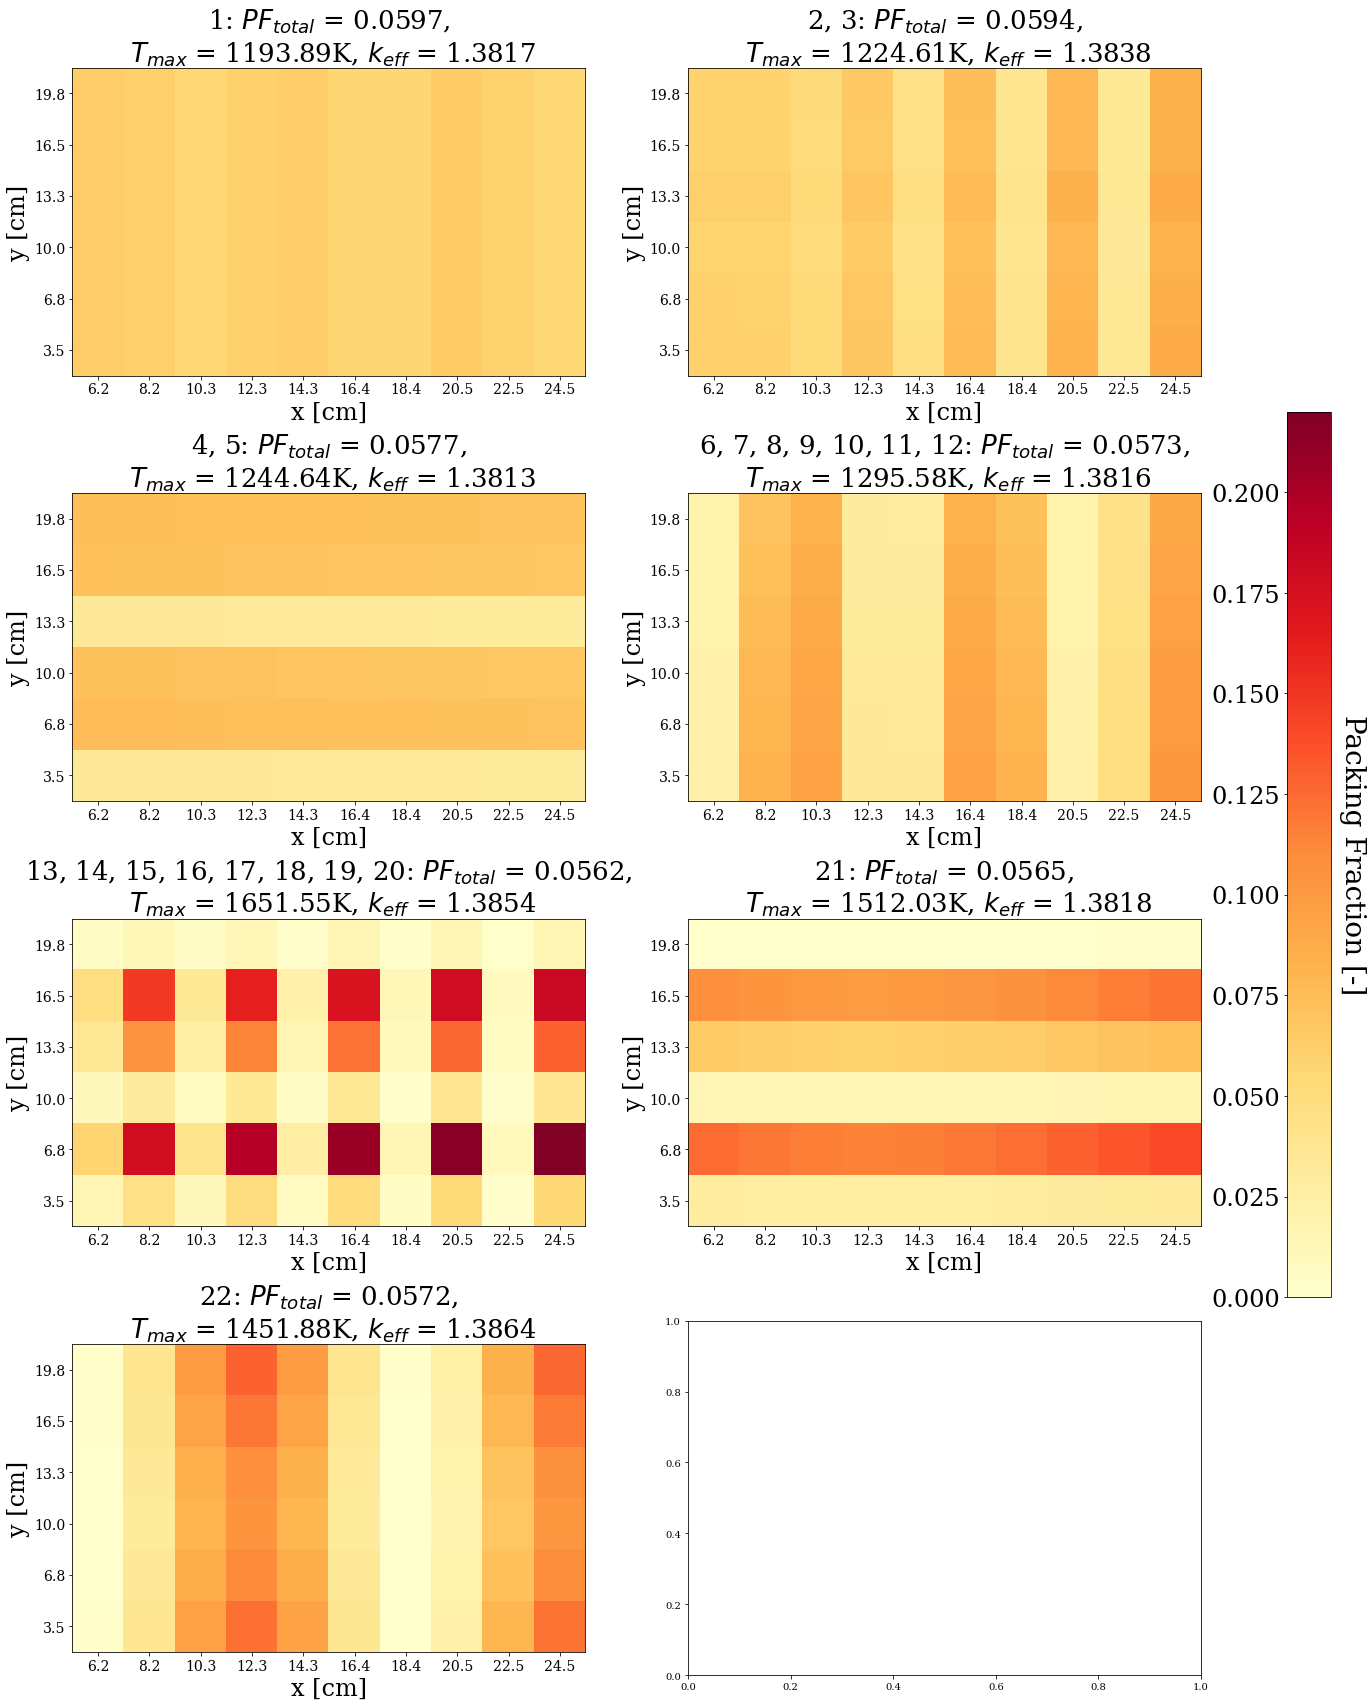
\includegraphics[width=0.95\linewidth]{assem-obj-2-pftemp-pareto-distr.png}
        \caption{TRISO distribution for the 22 reactor models on the Pareto front.
        Numbered reactor models correspond to numbered crosses in the plot above. }
        \label{fig:assem-obj-2-pftemp-pareto-distr} 
    \end{subfigure}
    \caption{(contd.) Simulation a-2a -- ROLLO two-objective optimization to minimize total fuel 
    packing fraction ($PF_{total}$) and maximum temperature ($T_{max}$) in 
    the one-third assembly. 
    Input parameters varied: total fuel packing fraction ($PF_{total}$) and TRISO 
    packing fraction distribution ($\rho_{TRISO}(\vec{r})$).}
\end{figure}

Figure \ref{fig:assem-obj-2-pftemp-pareto} shows that minimize $PF_{total}$ and 
minimize $T_{max}$ are contrasting objectives. 
In Figure \ref{fig:assem-obj-2-pftemp}, the one-third assembly model with the 
most-minimized $PF_{total}$ and highest $T_{max}$ are reactor models 13 to 20. 
These models have an oscillating TRISO distribution along the 
x-axis and y-axis, and a packing fraction standard deviation of $0.066$ across the 
one-third assembly. 
Along the x-axis, the distribution peaks at the even fuel cell columns (at 8.2cm,  
and 12.3cm, 16.4cm, 20.5cm, and 24.5cm) and has minimum points at the odd fuel cell 
columns (at 6.2cm, 10.3cm, 14.3cm, 18.4cm, and 22.5cm).
The even fuel cell columns have a $\sim0.18$ y-axis variation with peaks of 
$PF\approx0.21$. 

In Figure \ref{fig:assem-obj-2-pftemp}, the one-third assembly model with the 
most-minimized $T_{max}$ and highest $PF_{total}$ is reactor model 1. 
Reactor model 1 has an almost constant TRISO packing fraction distribution with 
a packing fraction standard deviation of $0.004$ across the one-third assembly. 
The one-third assembly model that visually from the Pareto Front (Figure 
\ref{fig:assem-obj-2-pftemp-pareto}) minimizes both $PF_{total}$ and $T_{max}$ 
to an equal extent are reactor models 4 and 5. 
Reactor models 4 and 5 have an oscillating TRISO distribution along the y-axis and 
a packing fraction standard deviation of $0.018$ across the one-third assembly. 
Along the y-axis, the distribution peaks at the 2nd, 3rd, 5th, and 6th rows 
(at 6.8cm, 10.0cm, 16.5cm, and 19.8cm) with $PF\approx0.07$ and has minimum points at 
the 1st and 4th rows (at 3.5cm and 13.3cm) with $PF\approx0.03$. 
Section \ref{sec:assem-discussion-multi} discusses and explains simulation a-2a's 
results.

\subsection{a-2b: Minimize $PF_{total}$ and $PPF_{fuel}$}
\label{sec:a-2b}
This section reports results from the two-objective optimization simulation a-2b; the 
objectives minimized are total fuel packing fraction ($PF_{total}$) and fuel-normalized 
power peaking factor ($PPF_{fuel}$) in the one-third assembly.  
Table \ref{tab:simulationa2b} shows simulation a-2b's optimization problem parameters. 
\begin{table}[htbp!]
    \centering
    \onehalfspacing
    \caption{Simulation a-2b Optimization Problem Parameters}
	\label{tab:simulationa2b}
    \footnotesize
    \begin{tabular}{l|p{5.3cm}}
    \hline 
    \multicolumn{2}{c}{\textbf{Two Objectives: Simulation a-2b}} \\
    \hline 
    \textbf{Objectives} & Minimize $PF_{total}$ \\
    & Minimize $PPF_{fuel}$ \\
    \hline 
    \textbf{Input parameter variations} & $0.05 \leq PF_{total} \leq 0.07$ \\
    & $\rho_{TRISO}(\vec{r})$: $0 \leq a \leq 2$, $0 \leq d \leq 2$\\
    & $\rho_{TRISO}(\vec{r})$: $0 \leq b \leq \frac{\pi}{2}$, $0 \leq e \leq \frac{\pi}{2}$\\
    & $\rho_{TRISO}(\vec{r})$: $0 \leq c \leq 2\pi$, $0 \leq f \leq 2\pi$\\
    \hline
    \textbf{Constraints} & $k_{eff} \geq 1.38$\\ 
    \hline 
    \textbf{Genetic algorithm parameters} & Population size: 128 \\
    & Generations: 5 \\
    \hline
    \end{tabular}
\end{table}

Table \ref{tab:a2b-hypervolume} shows the hypervolume value at each generation, 
confirming that simulation a-2b converges by generation 5. 
\begin{table}[htbp!]
    \centering
    \onehalfspacing
    \caption{Simulation a-2b hypervolume values at each generation.}
	\label{tab:a2b-hypervolume}
    \footnotesize
    \begin{tabular}{ll}
    \hline 
    \multicolumn{2}{c}{\textbf{Two Objectives: Simulation a-2b}} \\
    \multicolumn{2}{c}{Reference point: (0.07, 1.9)} \\
    \hline 
    \textbf{Generation} & \textbf{Hypervolume [-]} \\
    \hline
    1 & 0.00989 \\
    2 & 0.00991 \\
    3 & 0.00997 \\
    4 & 0.01054\\
    5 & 0.01058\\
    \hline
    \end{tabular}
\end{table}

Figure \ref{fig:assem-obj-2-pfppf-pareto} shows a plot of the final generation's reactor 
models' $PF_{total}$ against $PPF_{fuel}$; crosses mark the reactor models that fall on 
the Pareto front.
Figure \ref{fig:assem-obj-2-pfppf-pareto-distr} shows the 12 TRISO packing fraction 
distributions that fall on the Pareto front. 
\begin{figure}[htbp!]
    \begin{subfigure}{\textwidth}
        \centering
        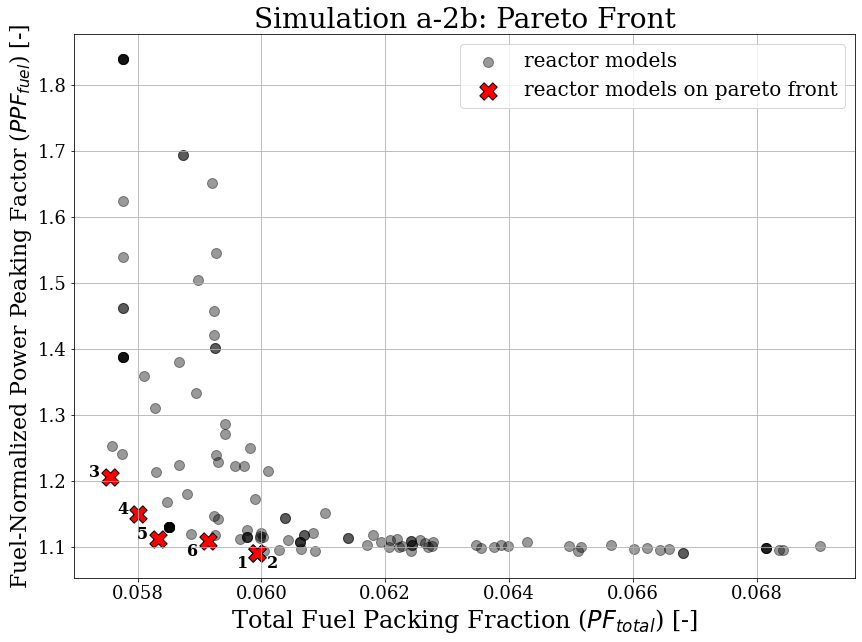
\includegraphics[width=\linewidth]{assem-obj-2-pfppf-pareto.png}
        \caption{Plot of final generation's reactor models' $PF_{total}$ against 
        $PPF_{fuel}$. 
        Crosses indicate the reactor models on the Pareto front. Annotated numbers 
        on each cross correspond to TRISO distributions in Figure 
        \ref{fig:assem-obj-2-pfppf-pareto-distr}.}
        \label{fig:assem-obj-2-pfppf-pareto} 
    \end{subfigure}
    \caption{Simulation a-2b -- ROLLO two-objective optimization to minimize total fuel 
    packing fraction ($PF_{total}$) and normalized power peaking factor ($PPF_{fuel}$) 
    in the \gls{AHTR} one-third assembly. 
    Input parameters varied: $PF_{total}$ and TRISO 
    packing fraction distribution ($\rho_{TRISO}(\vec{r})$).}
    \label{fig:assem-obj-2-pfppf}
\end{figure}
\begin{figure}[htbp!]
    \ContinuedFloat
    \begin{subfigure}{\textwidth}
        \centering
        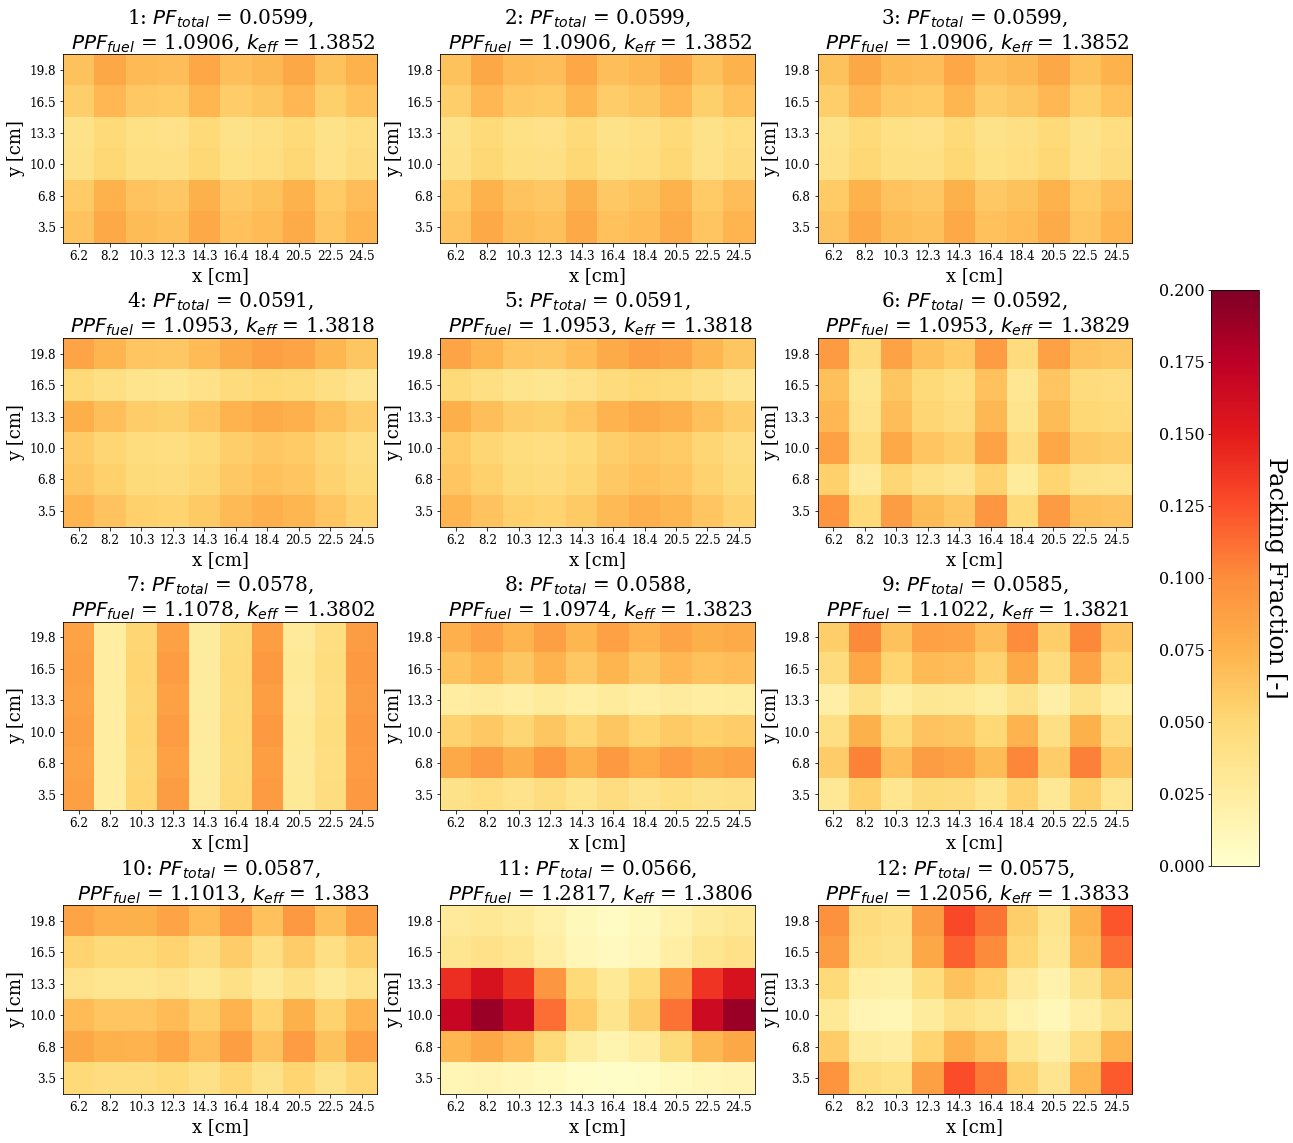
\includegraphics[width=\linewidth]{assem-obj-2-pfppf-pareto-distr.png}
        \caption{TRISO distribution for the 12 reactor models on the Pareto front.
        Numbered reactor models correspond to numbered crosses in Figure 
        \ref{fig:assem-obj-2-pfppf-pareto}. }
        \label{fig:assem-obj-2-pfppf-pareto-distr} 
    \end{subfigure}
    \caption{(contd.) Simulation a-2b -- ROLLO two-objective optimization to minimize total fuel 
    packing fraction ($PF_{total}$) and normalized power peaking factor ($PPF_{fuel}$) 
    in the \gls{AHTR} one-third assembly. 
    Input parameters varied: $PF_{total}$ and TRISO 
    packing fraction distribution ($\rho_{TRISO}(\vec{r})$).}
\end{figure}

Figure \ref{fig:assem-obj-2-pfppf-pareto} shows that minimize $PF_{total}$ and 
minimize $PPF_{fuel}$ are contrasting objectives. 
In Figure \ref{fig:assem-obj-2-pfppf}, the one-third assembly model with 
the most-minimized $PF_{total}$ and highest $PPF_{fuel}$ is reactor model 11. 
Reactor model 11 has an oscillating TRISO distribution along the 
x-axis and y-axis, and a packing fraction standard deviation of $0.053$ across the 
one-third assembly. 
Along the y-axis, the distribution peaks at the 3rd and 4th fuel cell rows (at 
10.0cm amd 13.3cm) and has minimum points at the 1st, 5th, and 6th fuel cell rows 
(at 3.5cm, 16.5cm, 19.8cm). 
The 3rd and 4th rows have the largest x-axis variation of $\sim0.14$ with 
peaks of $PF\approx0.17$. 
The 1st, 5th, and 6th row has the smallest x-axis variation of $\sim0.02$ with 
minimums of $PF\approx0.005$. 

In Figure \ref{fig:assem-obj-2-pfppf}, the one-third assembly model with 
the most-minimized $PPF_{fuel}$ and highest $PF_{total}$ is reactor model 1.
Reactor model 1 has an oscillating TRISO distribution along the 
x-axis and y-axis and a packing fraction standard deviation of $0.013$ across the 
one-third assembly.
Along the x-axis, the distribution peaks at the 2nd, 5th, and 8th fuel cell columns (at 
8.2cm, 14.3cm, and 20.5cm) and has minimum points at the 1st, 6th, and 9th (at 6.2cm, 
16.4cm, and 22.5cm).
The 2nd, 5th, and 8th columns have the largest y-axis variation of $\sim0.034$ with 
peaks of $PF\approx0.08$.
The 1st, 6th, and 9th columns have the smallest y-axis variation of $\sim0.027$ with 
minimums of $PF\approx0.038$. 
On the y-axis, the distribution has peaks at the top and bottom row (at 3.5cm and 
19.8cm) and has a minimum point in the center rows (at 10.0cm and 13.3cm).
The top and bottom row have the largest x-axis variation of $\sim0.018$ with 
peaks of $PF\approx0.08$.
The center rows have the smallest x-axis variation of $\sim0.011$ with minimums 
of $PF\approx0.038$. 

The one-third assembly model that visually from the Pareto Front (Figure 
\ref{fig:assem-obj-2-pfppf-pareto}) minimizes both $PF_{total}$ and $PPF_{fuel}$ 
to an equal extent is reactor model 5. 
Similar to reactor models 11 and 1, reactor model 5 has an oscillating TRISO 
distribution along the x-axis and y-axis and it has a packing fraction 
standard deviation of $0.013$ across the one-third assembly.
Along the x-axis, the distribution peaks at the 1st and 7th fuel cell columns 
(at 6.2cm and 18.4cm) and has minimum points in the 3rd, 4th, and 10th fuel cell 
columns (at 10.3cm, 12.3cm, and 24.5cm).
Along the x-axis, all the columns have a similar x-axis variation of $\sim0.03$.
Along the y-axis, the distribution peaks at the 4th and 6th fuel cell rows (at 13.3cm 
and 19.8cm) and has minimum points at the 5th fuel row (at 16.5cm). 
The 4th and 6th rows have the largest x-axis variation of $\sim0.024$ with peaks of 
$PF\approx0.08$. 
The 5th row has the smallest x-axis variation of $\sim0.015$ with minimums of 
$PF\approx0.035$. 
Sections \ref{sec:assem-discussion-multi} discusses and explains simulation a-2b's 
results.

\subsection{a-2c: Minimize $T_{max}$ and $PPF_{fuel}$}
\label{sec:a-2c}
This section reports results from the two-objective optimization simulation a-2c; the 
objectives minimized are maximum temperature ($T_{max}$) and fuel-normalized power 
peaking factor ($PPF_{fuel}$) in the one-third assembly.  
Table \ref{tab:simulationa2c} shows simulation a-2c's optimization problem parameters. 
\begin{table}[htbp!]
    \centering
    \onehalfspacing
    \caption{Simulation a-2c Optimization Problem Parameters}
	\label{tab:simulationa2c}
    \footnotesize
    \begin{tabular}{l|p{5.3cm}}
    \hline 
    \multicolumn{2}{c}{\textbf{Two Objectives: Simulation a-2c}} \\
    \hline 
    \textbf{Objectives} & Minimize $T_{max}$ \\
    & Minimize $PPF_{fuel}$ \\
    \hline 
    \textbf{Input parameter variations}
    & $\rho_{TRISO}(\vec{r})$: $0 \leq a \leq 2$, $0 \leq d \leq 2$\\
    & $\rho_{TRISO}(\vec{r})$: $0 \leq b \leq \frac{\pi}{2}$, $0 \leq e \leq \frac{\pi}{2}$\\
    & $\rho_{TRISO}(\vec{r})$: $0 \leq c \leq 2\pi$, $0 \leq f \leq 2\pi$\\
    \hline
    \textbf{Constraints} & $k_{eff} \geq 1.38$\\ 
    & $PF_{total} = 0.06$\\
    \hline 
    \textbf{Genetic algorithm parameters} & Population size: 128 \\
    & Generations: 2 \\
    \hline
    \end{tabular}
\end{table}

Table \ref{tab:a2c-hypervolume} shows the hypervolume value at each generation, 
confirming that simulation a-2c converges by generation 2. 
\begin{table}[htbp!]
    \centering
    \onehalfspacing
    \caption{Simulation a-2c hypervolume values at each generation.}
	\label{tab:a2c-hypervolume}
    \footnotesize
    \begin{tabular}{ll}
    \hline 
    \multicolumn{2}{c}{\textbf{Two Objectives: Simulation a-2c}} \\
    \multicolumn{2}{c}{Reference point: (1700, 1.5)} \\
    \hline 
    \textbf{Generation} & \textbf{Hypervolume [-]} \\
    \hline
    1 & 210.685 \\
    2 & 210.685 \\
    \hline
    \end{tabular}
\end{table}

Figure \ref{fig:assem-obj-2-tempppf-pareto} shows a plot of the final generation's reactor 
models' $T_{max}$ against $PPF_{fuel}$; crosses mark the reactor models that fall on 
the Pareto front.
Figure \ref{fig:assem-obj-2-tempppf-pareto-distr} shows the one TRISO packing fraction 
distribution in the final generation that falls on the Pareto front. 
Figure \ref{fig:assem-obj-2-tempppf-min-tempppf} illustrates the one \gls{AHTR} one-third 
assembly model on the Pareto front. 
\begin{figure}[htbp!]
    \centering
    \begin{subfigure}{\textwidth}
        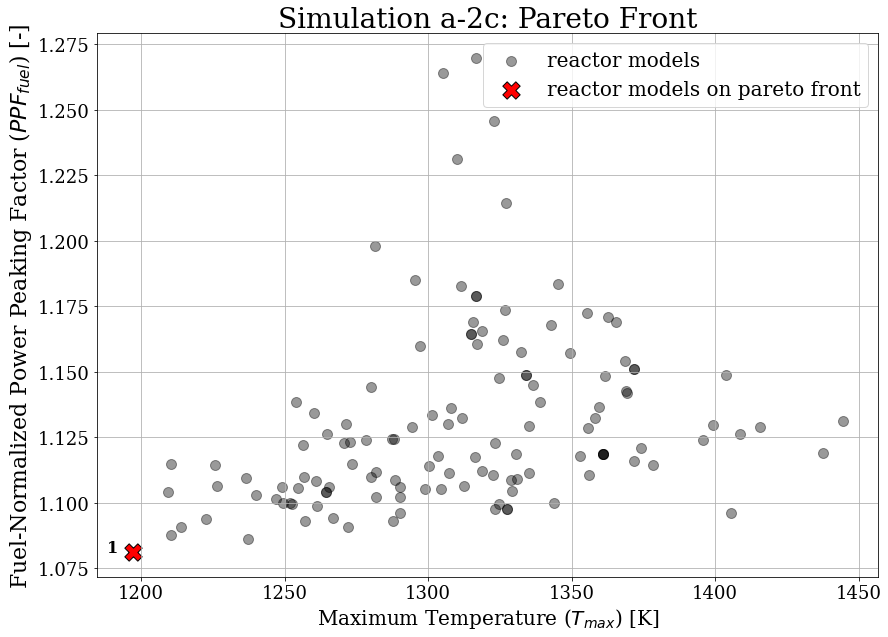
\includegraphics[width=\linewidth]{assem-obj-2-tempppf-pareto.png}
        \caption{Plot of final generation's reactor models' $T_{max}$ against 
        $PPF_{fuel}$. 
        Crosses indicate the reactor models on the Pareto front. Annotated numbers 
        on each cross correspond to TRISO distributions in the plot below.}
        \label{fig:assem-obj-2-tempppf-pareto} 
    \end{subfigure}
    \caption{Simulation a-2c -- ROLLO two-objective optimization to minimize 
    one-third assembly's maximum temperature ($T_{max}$) and fuel-normalized power peaking factor 
    ($PPF_{fuel}$) in the \gls{AHTR} one-third assembly. 
    Input parameters varied: TRISO packing fraction distribution ($\rho_{TRISO}(\vec{r})$).}
    \label{fig:assem-obj-2-tempppf}
\end{figure}
\begin{figure}[htbp!]
    \ContinuedFloat
    \begin{subfigure}{\textwidth}
        \centering
        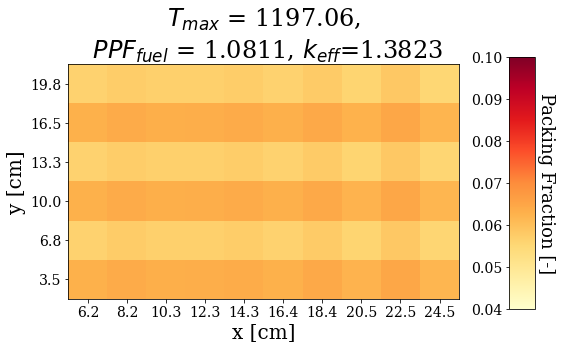
\includegraphics[width=0.7\linewidth]{a-2c-most-minimized.png}
        \caption{TRISO distribution for the 1 reactor model on the Pareto front.
        Numbered reactor models correspond to numbered crosses in the plot above. }
        \label{fig:assem-obj-2-tempppf-pareto-distr} 
    \end{subfigure}
    \begin{subfigure}{\textwidth}
        \centering
        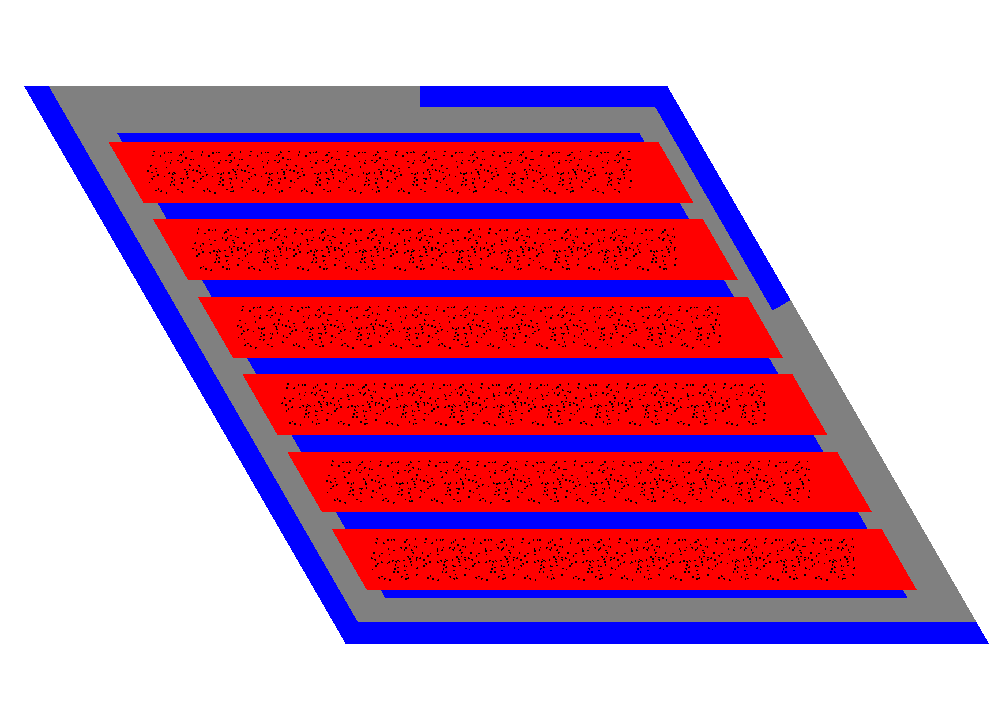
\includegraphics[width=0.7\linewidth]{assem-obj-2-tempppf-min-both.png}
        \caption{\gls{AHTR} one-third assembly model with the most-minimized $T_{max}$ and 
        $PPF_{fuel}$ (corresponds to the TRISO distribution in the above plot).}
        \label{fig:assem-obj-2-tempppf-min-tempppf} 
    \end{subfigure}
    \caption{(contd.) Simulation a-2c -- ROLLO two-objective optimization to minimize 
    one-third assembly's maximum temperature ($T_{max}$) and fuel-normalized power peaking factor 
    ($PPF_{fuel}$) in the \gls{AHTR} one-third assembly. 
    Input parameters varied: TRISO packing fraction distribution ($\rho_{TRISO}(\vec{r})$).}
\end{figure}

Figure \ref{fig:assem-obj-2-tempppf-pareto} shows that minimize $T_{max}$ and minimize 
$PPF_{fuel}$ are non-contrasting objectives, resulting in a single reactor model on the 
Pareto Front. 
Figure \ref{fig:assem-obj-2-tempppf-pareto-distr} shows the TRISO distribution that best 
minimizes both $T_{max}$ and $PPF_{fuel}$. 
The reactor model has a TRISO distribution oscillates along the y-axis and oscillates 
slightly on the x-axis, and a packing fraction standard deviation of $0.033$ across 
the one-third assembly. 
Along the y-axis, the distribution peaks at the odd rows (at 3.5cm, 10.0cm, and 16.5cm) 
with $PF\approx0.06$ and has minimum points at the even rows (at 6.8cm, 13.3cm, and 
19.8cm) with $PF\approx0.055$.
Sections \ref{sec:assem-discussion-multi} discusses and explains simulation a-2c's 
results.

\section{AHTR One-Third Assembly: Three-Objective Optimization Results}
\label{sec:assem-three-obj}
This section reports the \gls{AHTR} one-third assembly's \gls{ROLLO} three-objective 
optimization results. 
Table \ref{tab:assem-obj-breakdown} summarized the three-objective simulations in this 
section: a-3a, and a-3b. 

\subsection{a-3a: Variation of $PF_{total}$ and $\rho_{TRISO}(\vec{r})$}
\label{sec:a-3a}
This section reports results from the three-objective optimization simulation a-3a, 
with all objectives minimized: total fuel packing fraction ($PF_{total}$), 
maximum temperature ($T_{max}$), and fuel-normalized power peaking factor ($PPF_{fuel}$)
in the one-third assembly.  
The input parameters varied are $PF_{total}$ and TRISO packing fraction distribution 
($\rho_{TRISO}(\vec{r})$). 
Table \ref{tab:simulationa3a} shows simulation a-3a's optimization problem parameters. 
\begin{table}[htbp!]
    \centering
    \onehalfspacing
    \caption{Simulation a-3a optimization problem parameters.}
	\label{tab:simulationa3a}
    \footnotesize
    \begin{tabular}{l|p{5.3cm}}
    \hline 
    \multicolumn{2}{c}{\textbf{Three Objectives: Simulation a-3a}} \\
    \hline 
    \textbf{Objectives} & Minimize $PF_{total}$ \\
    & Minimize $T_{max}$ \\
    & Minimize $PPF_{fuel}$ \\
    \hline 
    \textbf{Input parameter variations} & $0.05 \leq PF_{total} \leq 0.07$ \\
    & $\rho_{TRISO}(\vec{r})$: $0 \leq a \leq 2$, $0 \leq d \leq 2$\\
    & $\rho_{TRISO}(\vec{r})$: $0 \leq b \leq \frac{\pi}{2}$, $0 \leq e \leq \frac{\pi}{2}$\\
    & $\rho_{TRISO}(\vec{r})$: $0 \leq c \leq 2\pi$, $0 \leq f \leq 2\pi$\\
    \hline
    \textbf{Constraints} & $k_{eff} \geq 1.38$\\ 
    \hline 
    \textbf{Genetic algorithm parameters} & Population size: 128 \\
    & Generations: 5 \\
    \hline
    \end{tabular}
\end{table}

Table \ref{tab:a3a-hypervolume} shows the hypervolume value at each generation, 
confirming that simulation a-3a converges by generation 5. 
\begin{table}[htbp!]
    \centering
    \onehalfspacing
    \caption{Simulation a-3a hypervolume values at each generation.}
	\label{tab:a3a-hypervolume}
    \footnotesize
    \begin{tabular}{ll}
    \hline 
    \multicolumn{2}{c}{\textbf{Three Objectives: Simulation a-3a}} \\
    \multicolumn{2}{c}{Reference point: (0.07, 1700,1.8)} \\
    \hline 
    \textbf{Generation} & \textbf{Hypervolume [-]} \\
    \hline
    1 & 4.0925 \\
    2 & 4.2233 \\
    3 & 4.4002 \\
    4 & 4.4250 \\
    5 & 4.5312 \\
    \hline
    \end{tabular}
\end{table}

Figure \ref{fig:assem-obj-3-2d} shows a plot of the final generation's reactor models' 
$PF_{total}$ against $T_{max}$ against $PPF_{fuel}$; crosses mark the reactor models 
that fall on the Pareto front.
Figure \ref{fig:assem-obj-3-distr} shows the 32 TRISO packing fraction distributions in 
the final generation that fall on the Pareto front. 
\begin{figure}[htbp!]
    \begin{subfigure}{\textwidth}
        \centering
        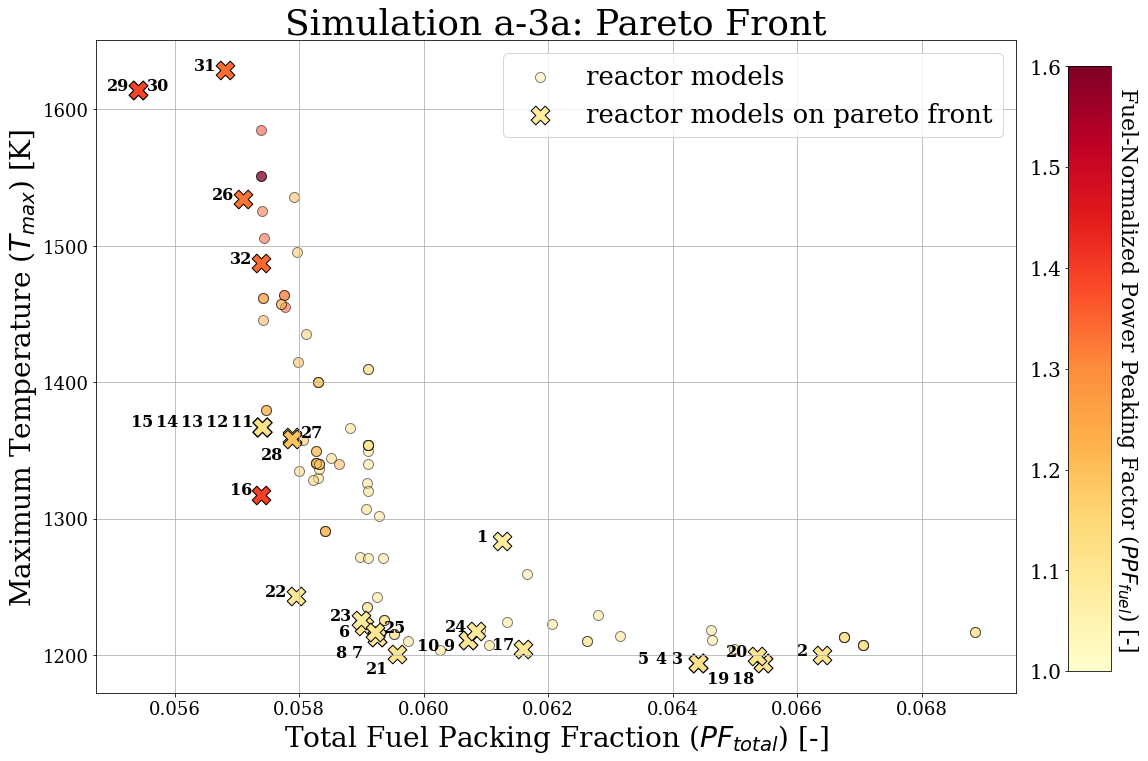
\includegraphics[width=\linewidth]{assem-obj-3-2d.png}
        \caption{Plot of final generation's reactor models' $PF_{total}$ against 
        $T_{max}$ against $PPF_{fuel}$ as a color dimension. 
        Crosses indicate the reactor models on the 
        Pareto front. Cross numbering correspond to TRISO distributions in Figure 
        \ref{fig:assem-obj-3-distr}.}
        \label{fig:assem-obj-3-2d} 
    \end{subfigure}
    \caption{Simulation a-3a -- ROLLO three-objective optimization to minimize total 
    fuel packing fraction ($PF_{total}$), maximum temperature ($T_{max}$), and 
    fuel-normalized power peaking factor ($PPF_{fuel}$) in the one-third assembly. 
    Input parameters varied: $PF_{total}$, TRISO packing fraction distribution
    ($\rho_{TRISO}(\vec{r})$).}
    \label{fig:assem-obj-3}
\end{figure}
\begin{figure}[htbp!]
    \ContinuedFloat
    \begin{subfigure}{\textwidth}
        \centering
        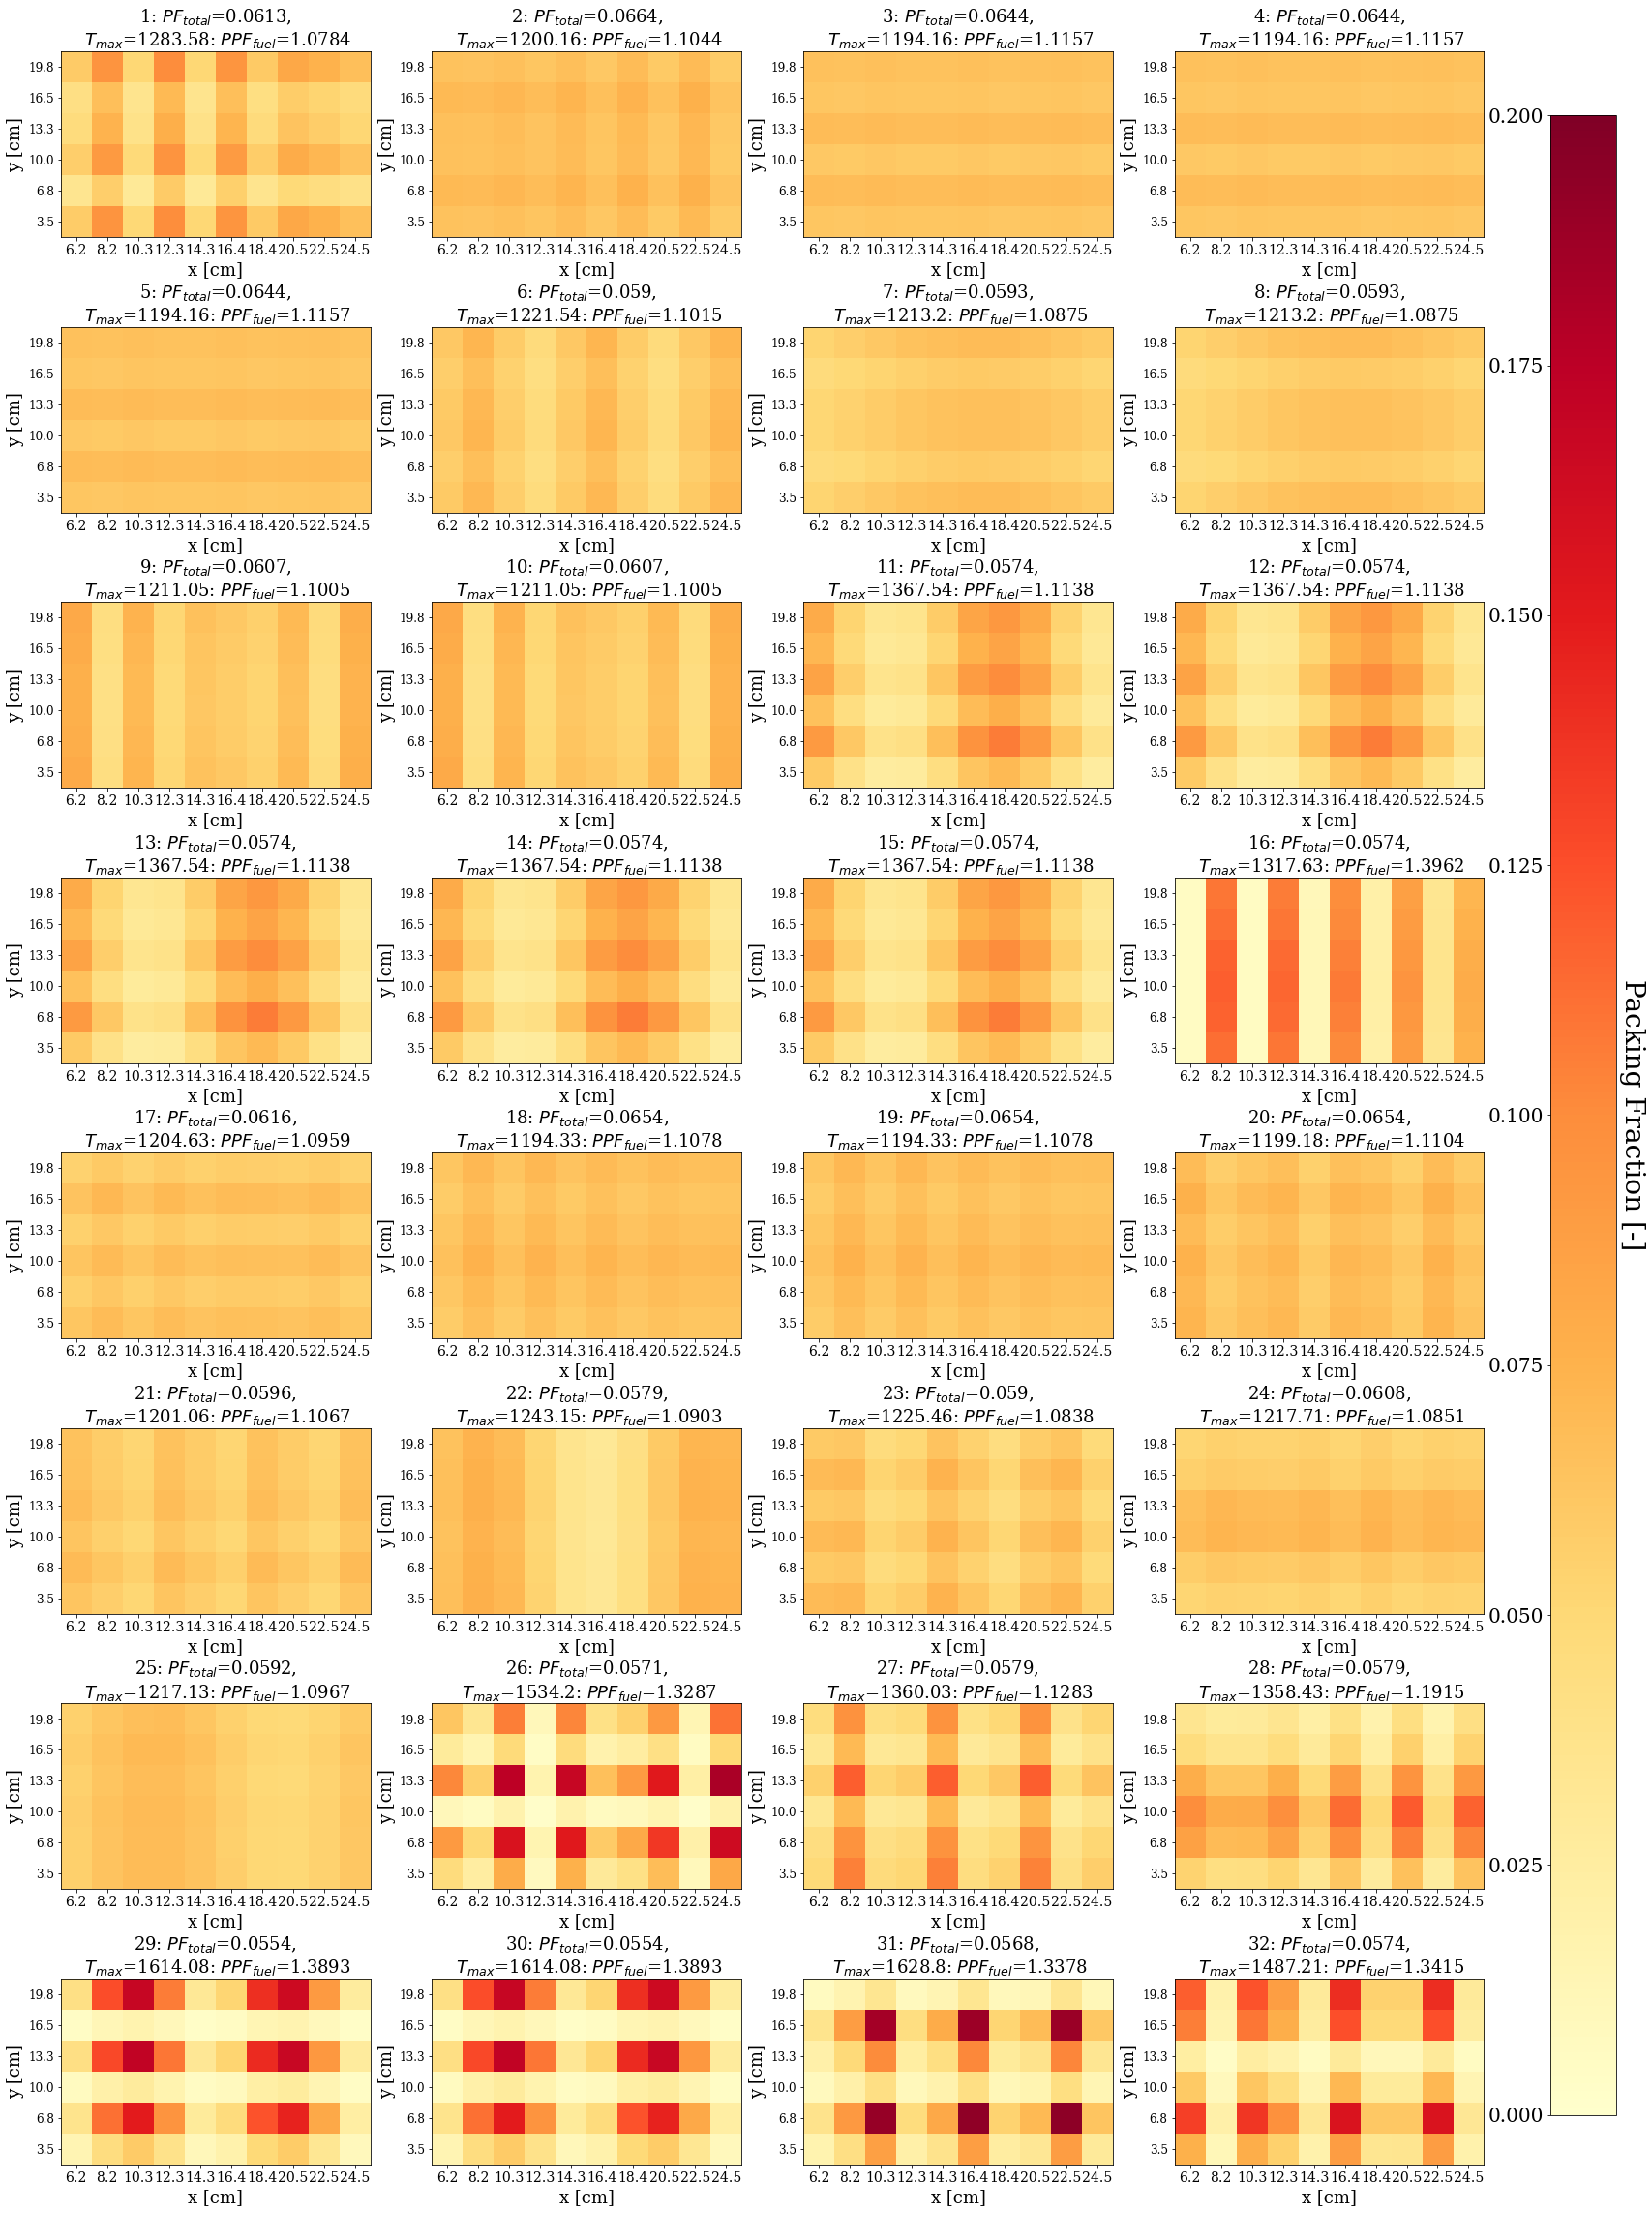
\includegraphics[width=\linewidth]{assem-obj-3-distr.png}
        \caption{TRISO distributions for the 32 reactor models on the Pareto front.
        Numbered reactor models correspond to numbered crosses in Figure 
        \ref{fig:assem-obj-3-2d}. }
        \label{fig:assem-obj-3-distr} 
    \end{subfigure}
    \caption{(contd.) Simulation a-3a -- ROLLO three-objective optimization to minimize 
    total fuel packing fraction ($PF_{total}$), maximum temperature ($T_{max}$),
    and fuel-normalized power peaking factor ($PPF_{fuel}$) in the one-third assembly. 
    Input parameters varied: $PF_{total}$, TRISO packing fraction distribution
    ($\rho_{TRISO}(\vec{r})$).}
\end{figure}

Figure \ref{fig:assem-obj-3} demonstrates that \gls{ROLLO} found 32 reactor models on 
simulation a-3a final generation's Pareto front. 
Figure \ref{fig:assem-obj-3-most-minimized} shows three reactor models on the 
Pareto front that most-minimized each objective, and one reactor model on the 
Pareto front that equally minimized all three objectives. 
I selected the equally minimized reactor model by visually studying Figure 
\ref{fig:assem-obj-3} and selecting a reactor model that is close to the origin 
and has a light yellow color dimension. 
Reactor model 30 most-minimized $PF_{total}$, reactor model 3 most-minimized $T_{max}$, 
reactor model 1 most-minimized $PPF_{fuel}$, and reactor model 22 equally minimized 
all three objectives. 
\begin{figure}[htbp!]
    \centering
    \begin{subfigure}{\textwidth}
    \centering
    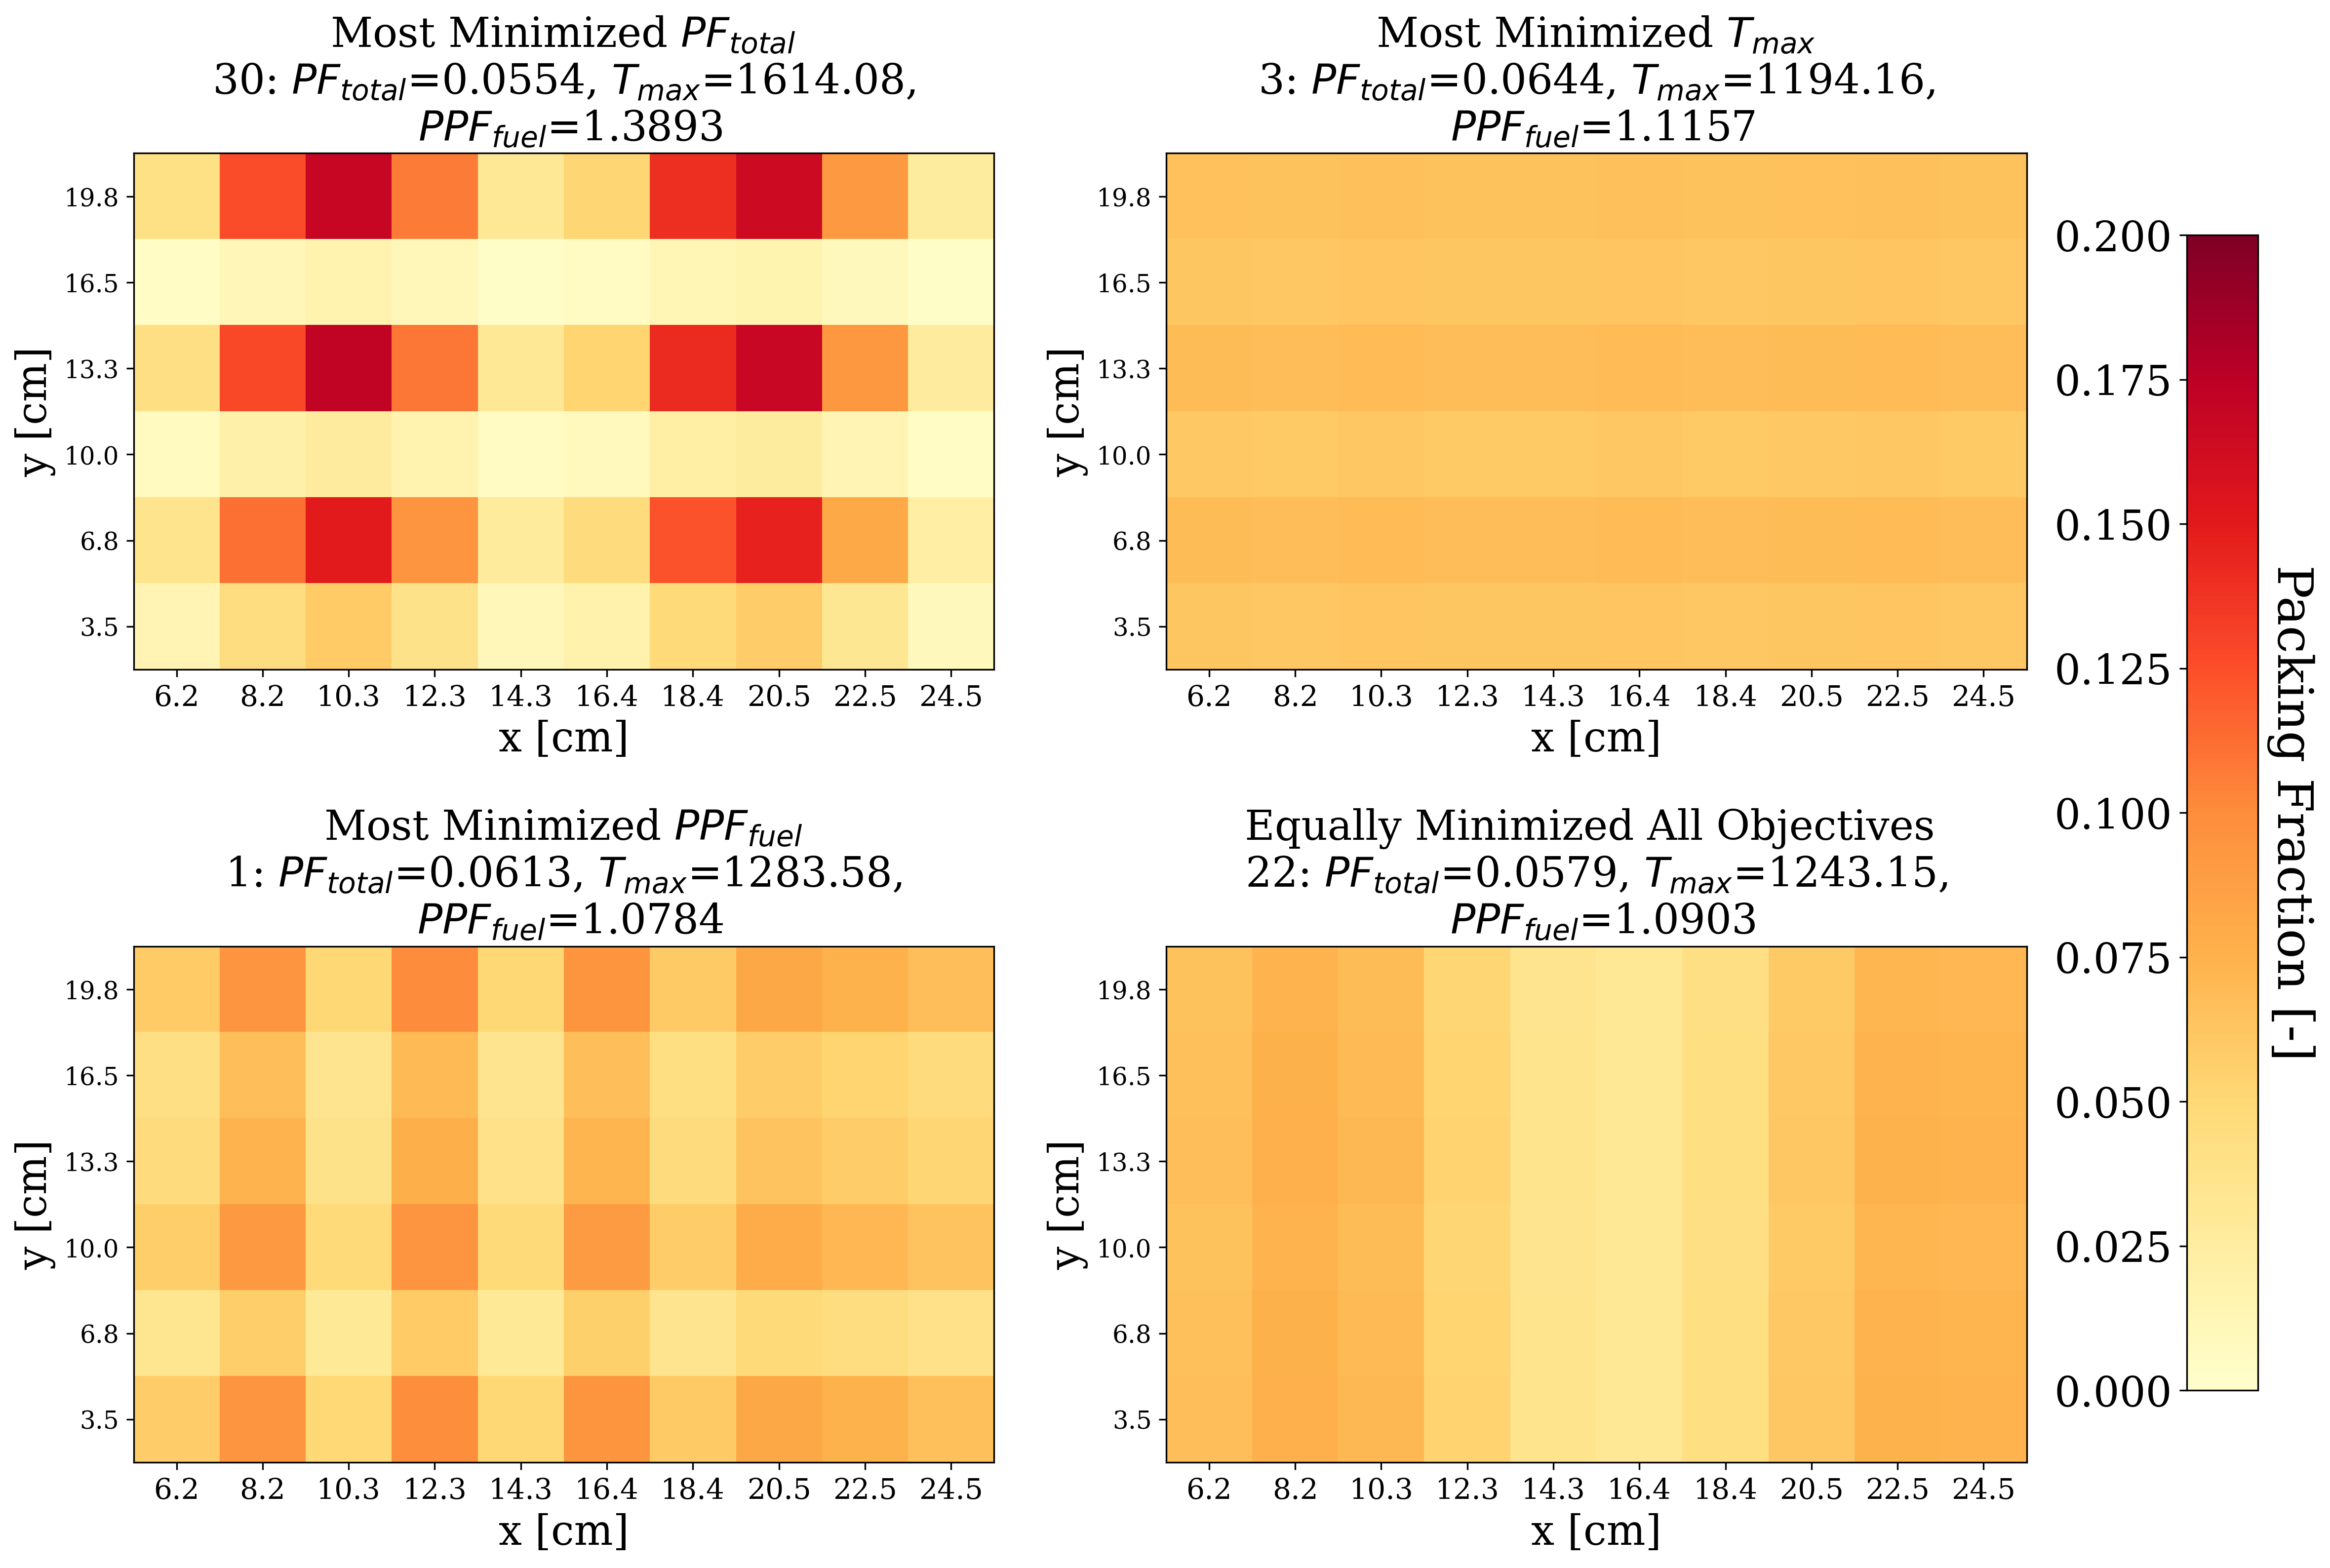
\includegraphics[width=\linewidth]{assem-obj-3-distr-most-minimized.png}
    \caption{TRISO packing fraction distributions.}
    \label{fig:assem-obj-3-most-minimized-distr}
    \end{subfigure}
    \caption{AHTR one-third assembly models and TRISO distributions for the three reactor 
    models on simulation a-3a's Pareto front that most-minimized each objective, and 
    one reactor model that equally minimized all three objectives.
    Simulation a-3a -- ROLLO three-objective optimization to minimize total fuel packing 
    fraction ($PF_{total}$), maximum temperature ($T_{max}$) and 
    normalized power peaking factor ($PPF_{fuel}$) in the one-third assembly. 
    Input parameters varied: $PF_{total}$, TRISO packing fraction distribution
    ($\rho_{TRISO}(\vec{r})$).}
    \label{fig:assem-obj-3-most-minimized}
\end{figure}
\begin{figure}[htbp!]
    \ContinuedFloat
    \begin{subfigure}{0.49\textwidth}
        \centering
        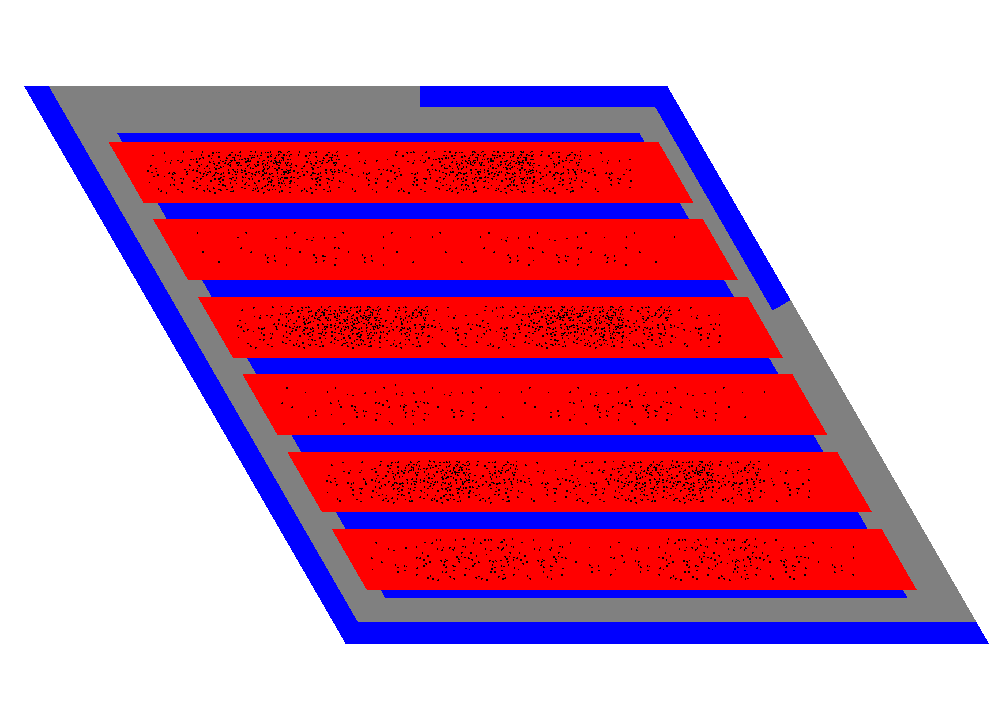
\includegraphics[width=\linewidth]{assem-obj-3-min-pf.png}
        \caption{\gls{AHTR} one-third assembly model with the most-minimized $PF_{total}$ 
        (reactor model 30).}
        \label{fig:assem-obj-3-min-pf} 
    \end{subfigure}
    \begin{subfigure}{0.49\textwidth}
        \centering
        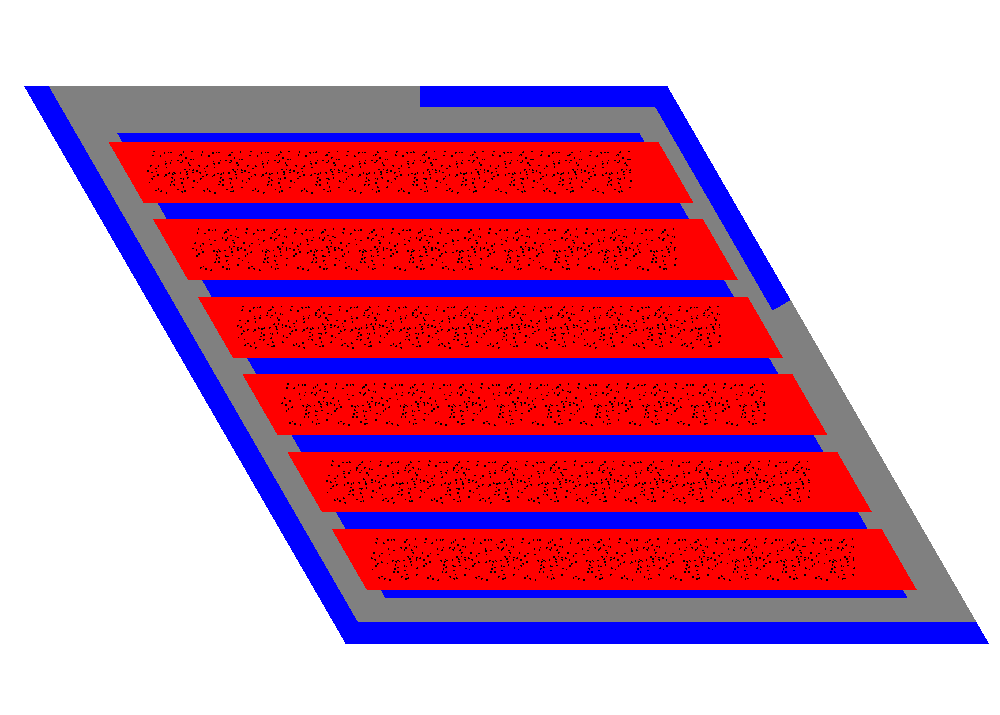
\includegraphics[width=\linewidth]{assem-obj-3-min-temp.png}
        \caption{\gls{AHTR} one-third assembly model with the most-minimized $T_{max}$
        (reactor model 3).}
        \label{fig:assem-obj-3-min-temp} 
    \end{subfigure}
    \begin{subfigure}{0.49\textwidth}
        \centering
        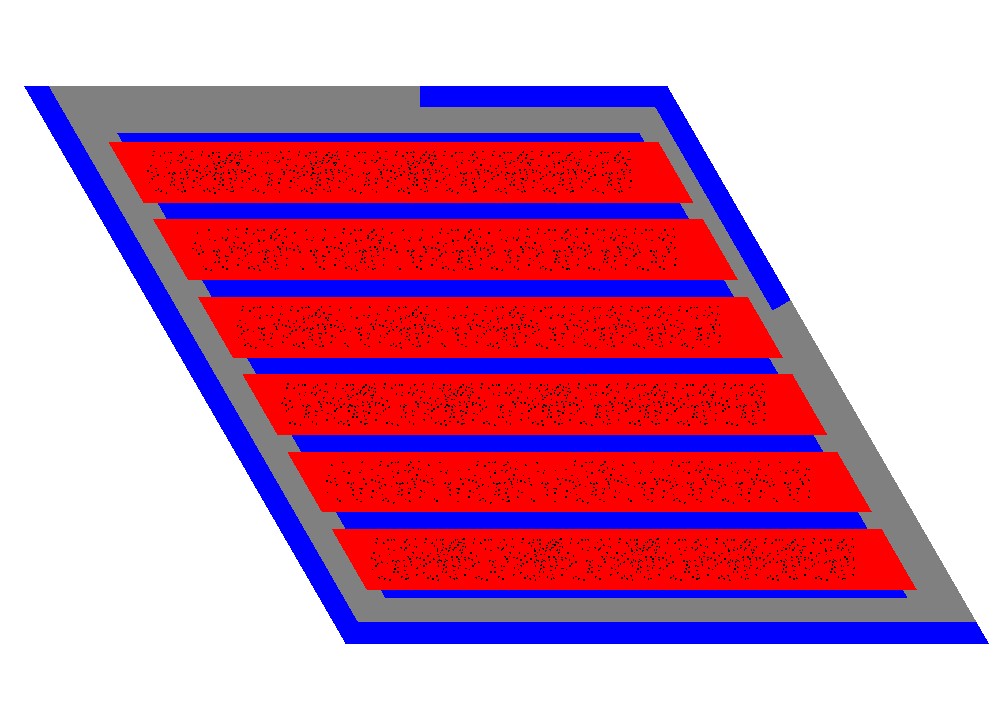
\includegraphics[width=\linewidth]{assem-obj-3-min-ppf.png}
        \caption{\gls{AHTR} one-third assembly model with the most-minimized $PPF_{fuel}$
        (reactor model 1).}
        \label{fig:assem-obj-3-min-ppf} 
    \end{subfigure}
    \begin{subfigure}{0.49\textwidth}
        \centering
        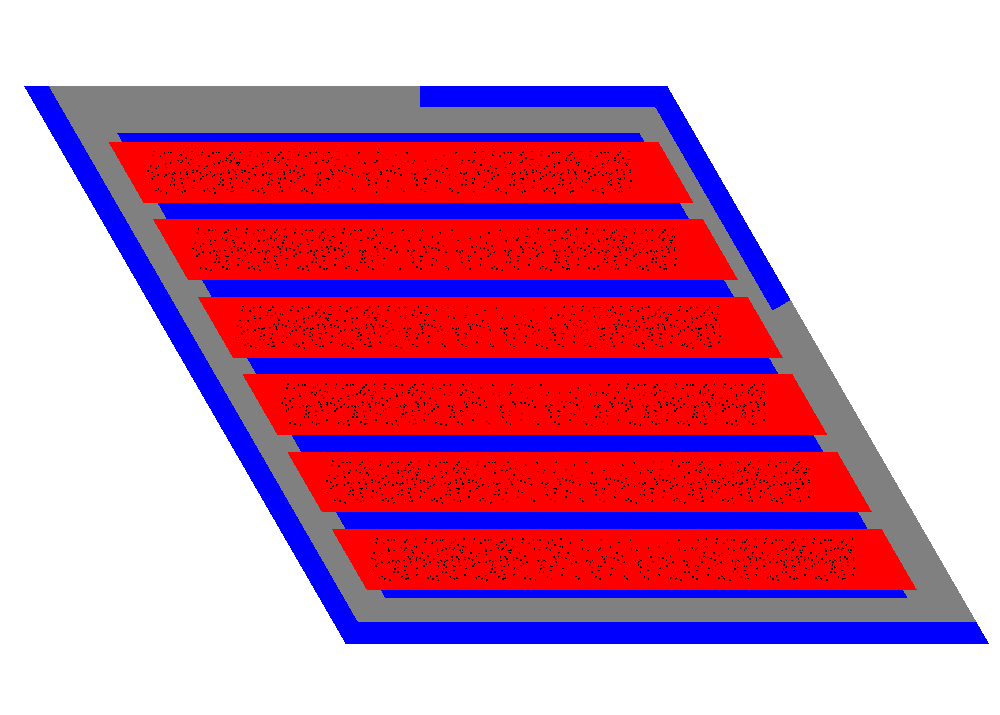
\includegraphics[width=\linewidth]{assem-obj-3-min-all.png}
        \caption{\gls{AHTR} one-third assembly model that equally minimized all objectives
        (reactor model 22).}
        \label{fig:assem-obj-3-min-all} 
    \end{subfigure}
    \begin{subfigure}{.4\textwidth}
    \vspace{1cm}
    \centering
    \resizebox{\textwidth}{!}{
    \fbox{\begin{tabular}{ll}
        \textcolor{fhrblue}{$\blacksquare$} & \gls{FLiBe} \\
        \textcolor{fhrgrey}{$\blacksquare$} & Graphite (Structure)\\
        \textcolor{fhrred}{$\blacksquare$} & Graphite (Fuel Plank) \\
        \textcolor{fhrblack}{$\blacksquare$} & TRISO particle 
        \end{tabular}}}
\end{subfigure}
    \caption{(contd.) AHTR one-third assembly models and TRISO distributions for the 
    three reactor models on simulation a-3a's Pareto front that most-minimized each 
    objective, and one reactor model that equally minimized all three objectives.
    Simulation a-3a -- ROLLO three-objective optimization to minimize total fuel packing 
    fraction ($PF_{total}$), maximum temperature ($T_{max}$) and 
    normalized power peaking factor ($PPF_{fuel}$) in the one-third assembly. 
    Input parameters varied: $PF_{total}$, TRISO packing fraction distribution
    ($\rho_{TRISO}(\vec{r})$).}
\end{figure}

In Figure \ref{fig:assem-obj-3-most-minimized-distr}, the one-third assembly model with 
the most-minimized $PF_{total}$ is reactor model 30 (also illustrated in Figure 
\ref{fig:assem-obj-3-min-pf}). 
Reactor model 30 has an oscillating TRISO distribution along the 
x-axis and y-axis, and a packing fraction standard deviation of $0.052$ across the 
one-third assembly. 
Along the y-axis, the distributions peaks at the even fuel cell rows (at 6.8cm, 
13.3cm, and 19.8cm) and has minimum points at the odd fuel cell rows (at 3.5cm, 
10.0cm, and 16.5cm). 
The even fuel cell rows have a $\sim0.14$ x-axis variation with peaks of 
$PF\approx0.16$. 
The odd fuel cell rows have a $\sim0.02$ x-axis variation with minimums of 
$PF\approx0.005$. 

In Figure \ref{fig:assem-obj-3-most-minimized-distr}, the one-third assembly model with 
the most-minimized $T_{max}$ is reactor model 3 (also illustrated in Figure 
\ref{fig:assem-obj-3-min-temp}). 
Reactor model 3 has an almost constant TRISO packing fraction distribution with 
a packing fraction standard deviation of $0.003$ across the one-third assembly. 
In Figure \ref{fig:assem-obj-3-most-minimized-distr}, the one-third assembly model with 
the most-minimized $PPF_{fuel}$ is reactor model 1 (also illustrated in Figure 
\ref{fig:assem-obj-3-min-ppf}).
Reactor model 1 has an oscillating TRISO distribution along the 
x-axis and y-axis and a packing fraction standard deviation of $0.019$ across the 
one-third assembly.
Along the x-axis, the distribution peaks at the 2nd, 4th, and 6th fuel cell columns (at 
8.2cm, 12.3cm, and 16.4cm). 
These three fuel cell columns have a $\sim0.04$ y-axis variation with peaks of 
$PF\approx0.1$. 
Along the y-axis, the distribution peaks at the 1st, 3rd, and 6th fuel cell rows (at 
3.5cm, 10.0cm, and 19.8cm).
These three fuel cell rows have a $\sim0.05$ x-axis variation with peaks of 
$PF\approx0.1$. 

In Figure \ref{fig:assem-obj-3-most-minimized-distr}, the one-third assembly model that 
equally minimized all three objectives is reactor model 22 (also illustrated in Figure 
\ref{fig:assem-obj-3-min-all}).
Reactor model 22 has an oscillating TRISO distribution along x-axis, and a packing 
fraction standard deviation of $0.015$ across the one-third assembly. 
Along the x-axis, the distribution peaks at the 2nd, 9th, and 10th fuel cell columns 
(at 8.2cm, 22.5cm, and 24.5cm) with $PF\approx0.07$.
The distribution has minimum points at the 5th and 6th fuel cell columns (at 14.3cm, 
16.4cm) with $PF\approx0.03$.
Section \ref{sec:assem-discussion-multi} discusses and explains simulation a-3a's 
results.

\subsection{a-3b: Variation of $PF_{total}$, $\rho_{TRISO}(\vec{r})$, and Coolant 
Channel Shape}
\label{sec:a-3b}
This section reports results from the three-objective optimization simulation a-3b, 
with all objectives minimized: total fuel packing fraction ($PF_{total}$), maximum 
temperature ($T_{max}$), and fuel-normalized power peaking factor ($PPF_{fuel}$)
in the one-third assembly.  
The input parameters varied are $PF_{total}$, TRISO packing fraction distribution 
($\rho_{TRISO}(\vec{r})$), and coolant channel shape ($r_1, r_2, r_3, r_4,$ and $r_5$).  
Table \ref{tab:simulationa3b} shows simulation a-3b's optimization problem parameters. 
\begin{table}[htbp!]
    \centering
    \onehalfspacing
    \caption{Simulation a-3b optimization problem parameters.}
	\label{tab:simulationa3b}
    \footnotesize
    \begin{tabular}{l|p{6.5cm}}
    \hline 
    \multicolumn{2}{c}{\textbf{Three Objectives: Simulation a-3b}} \\
    \hline 
    \textbf{Objectives} & Minimize $PF_{total}$ \\
    & Minimize $T_{max}$ \\
    & Minimize $PPF_{fuel}$ \\
    \hline 
    \textbf{Input parameter variations} & $0.05 \leq PF_{total} \leq 0.07$ \\
    & $\rho_{TRISO}(\vec{r})$: $0 \leq a \leq 2$, $0 \leq d \leq 2$\\
    & $\rho_{TRISO}(\vec{r})$: $0 \leq b \leq \frac{\pi}{2}$, $0 \leq e \leq \frac{\pi}{2}$\\
    & $\rho_{TRISO}(\vec{r})$: $0 \leq c \leq 2\pi$, $0 \leq f \leq 2\pi$\\
    & coolant channel shape: $0.1<r_{1}<0.35$ \\
    & coolant channel shape: $0.1<r_{2}<0.35$ \\
    & coolant channel shape: $0.1<r_{3}<0.35$ \\
    & coolant channel shape: $0.1<r_{4}<0.35$ \\
    & coolant channel shape: $0.1<r_{5}<0.35$ \\
    \hline
    \textbf{Constraints} & $k_{eff} \geq 1.38$\\ 
    \hline 
    \textbf{Genetic algorithm parameters} & Population size: 128 \\
    & Generations: 6 \\
    \hline
    \end{tabular}
\end{table}

Table \ref{tab:a3b-hypervolume} shows the hypervolume value at each generation, 
confirming that simulation a-3b converges by generation 6. 
\begin{table}[htbp!]
    \centering
    \onehalfspacing
    \caption{Simulation a-3b hypervolume values at each generation.}
	\label{tab:a3b-hypervolume}
    \footnotesize
    \begin{tabular}{ll}
    \hline 
    \multicolumn{2}{c}{\textbf{Three Objectives: Simulation a-3b}} \\
    \multicolumn{2}{c}{Reference point: (0.06, 1260,1.5)} \\
    \hline 
    \textbf{Generation} & \textbf{Hypervolume [-]} \\
    \hline
    1 & 5.4961 \\
    2 & 5.6739 \\
    3 & 5.6876 \\
    4 & 5.8104 \\
    5 & 6.0023 \\
    6 & 6.0093 \\
    \hline
    \end{tabular}
\end{table}

Figure \ref{fig:assem-obj-3-all-2d} shows a plot of the final generation's reactor 
models' $PF_{total}$ against $T_{max}$ against $PPF_{fuel}$; crosses mark the reactor 
models that fall on the Pareto front.
Figure \ref{fig:assem-obj-3-all-distr} shows the 12 TRISO packing fraction distributions 
in the final generation that fall on the Pareto front. 
\begin{figure}[htbp!]
    \begin{subfigure}{\textwidth}
        \centering
        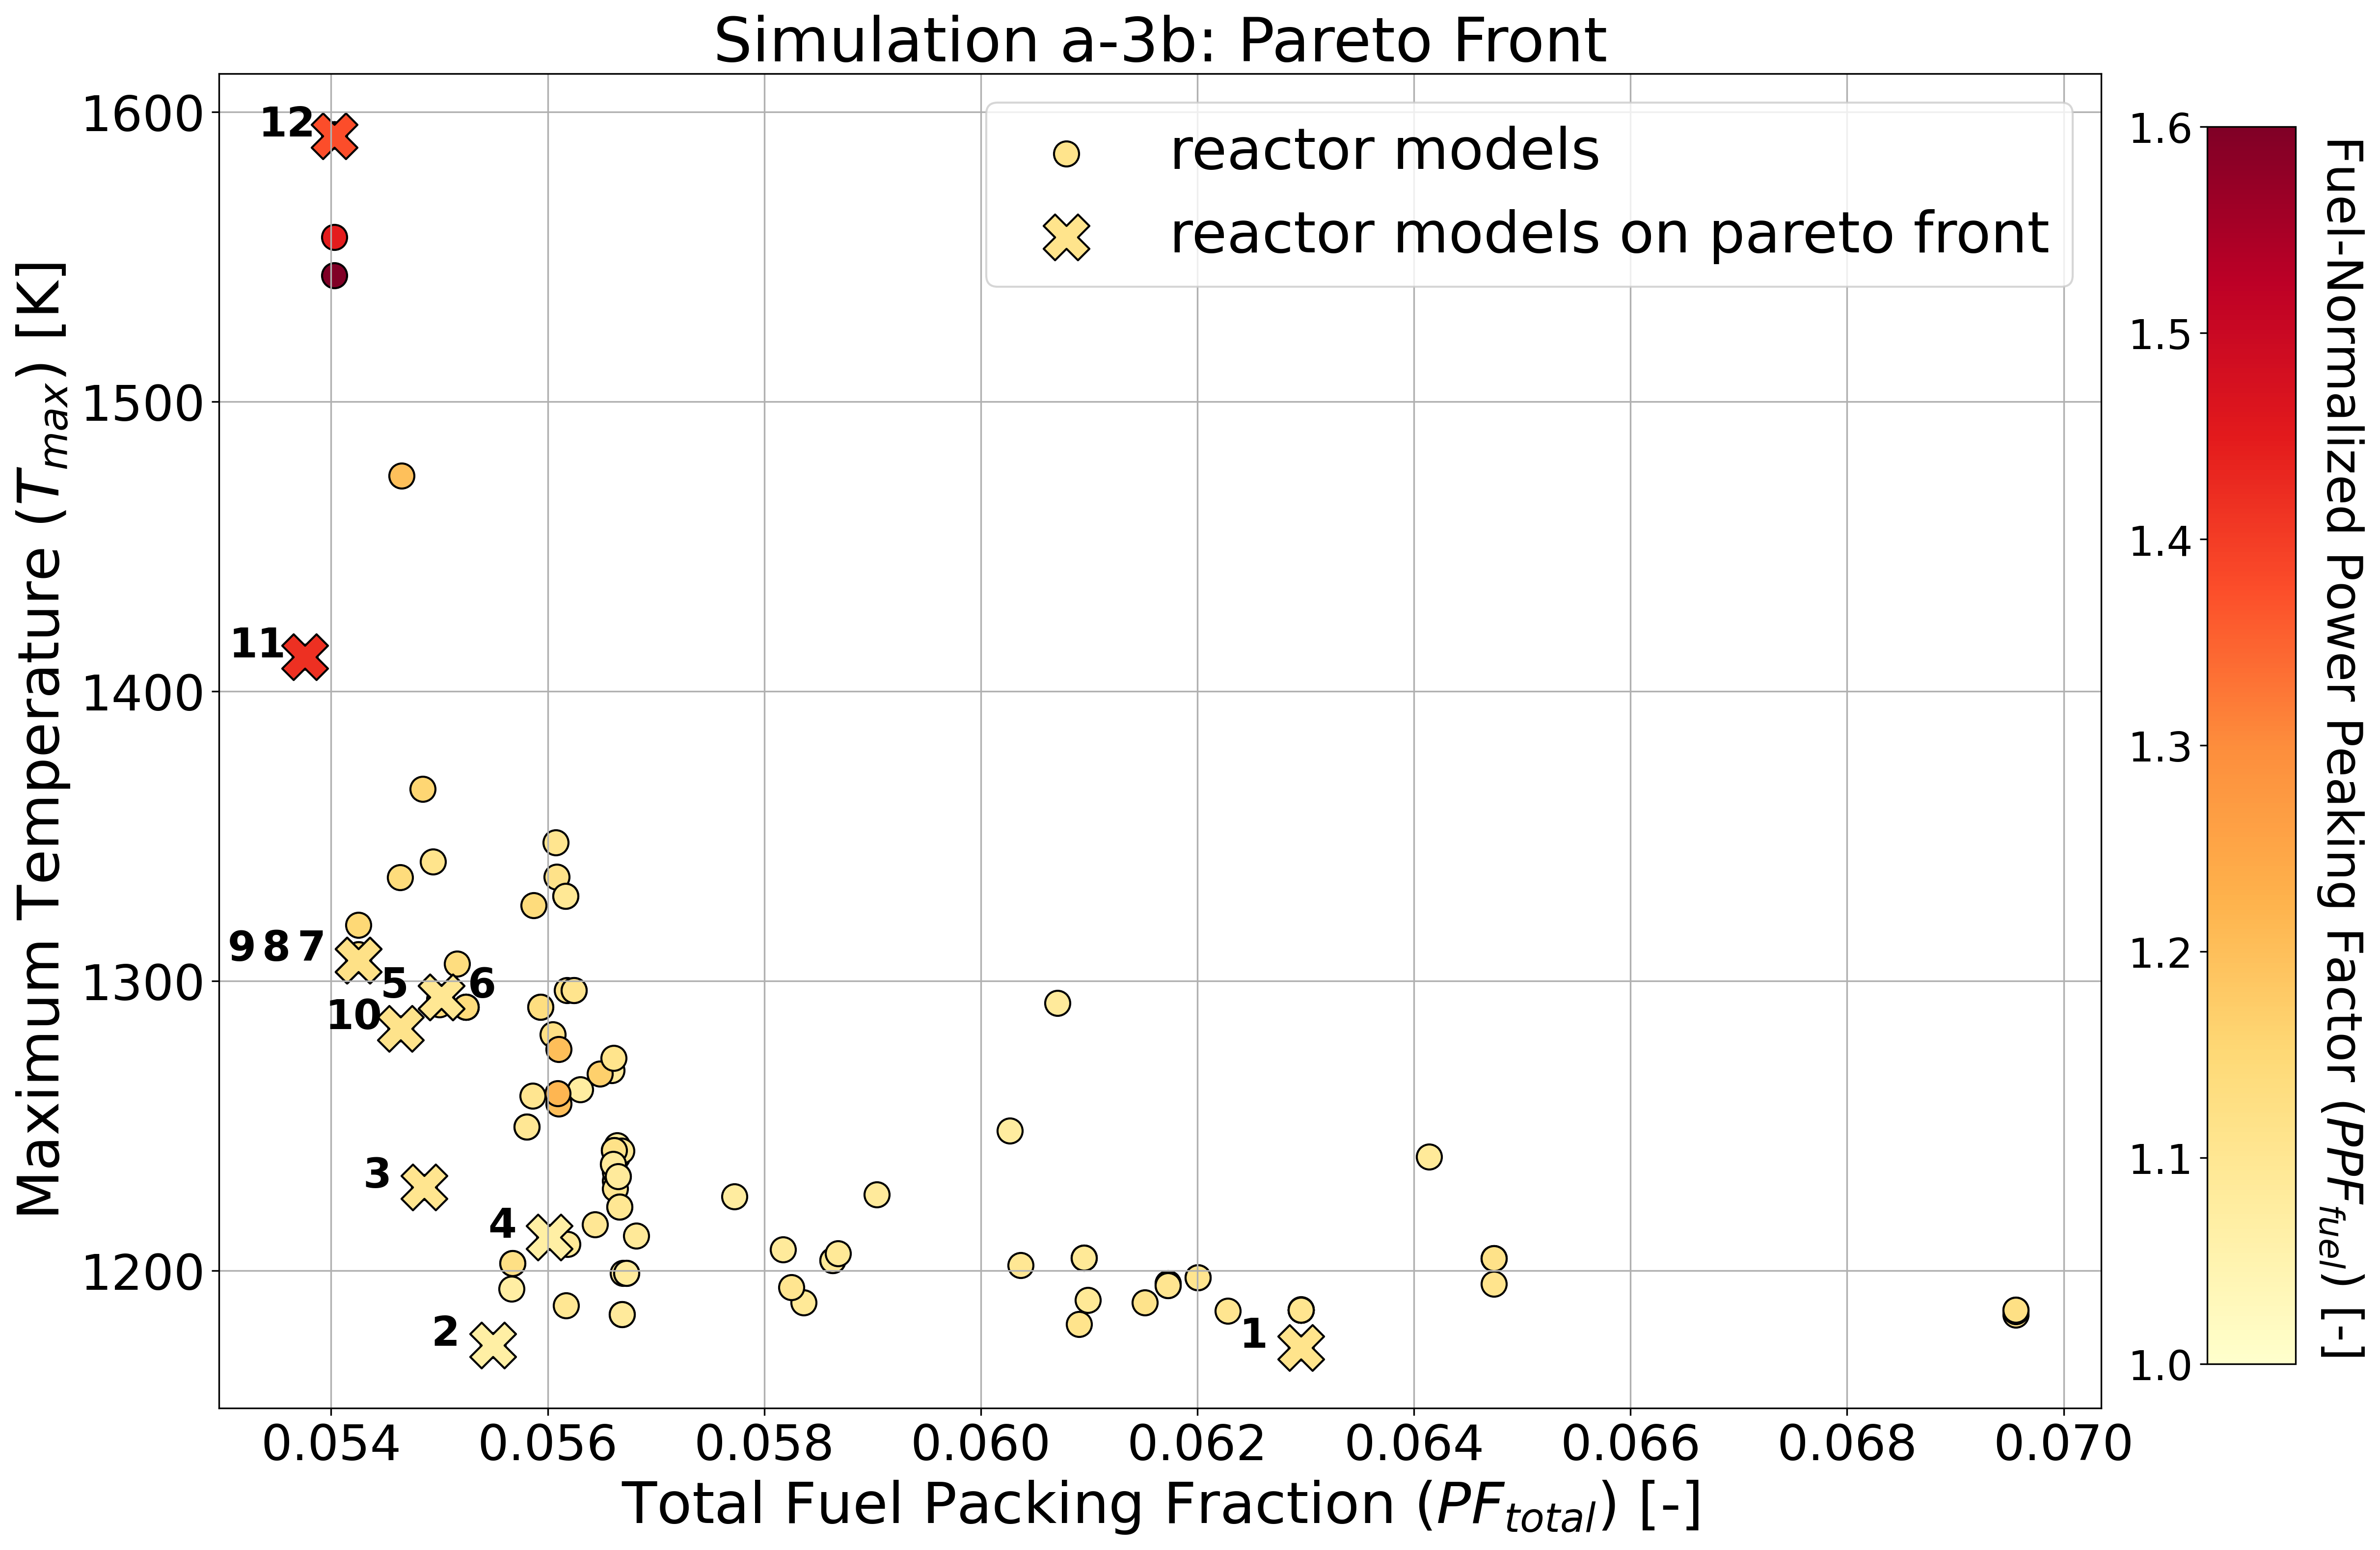
\includegraphics[width=\linewidth]{assem-obj-3-all-2d.png}
        \caption{Plot of final generation's reactor models' $PF_{total}$ against 
        $T_{max}$ against $PPF_{fuel}$ as a color dimension. 
        Crosses indicate the reactor models on the 
        Pareto front. Cross numbering correspond to TRISO distributions in Figure 
        \ref{fig:assem-obj-3-all-distr}.}
        \label{fig:assem-obj-3-all-2d} 
    \end{subfigure}
    \caption{Simulation a-3b -- ROLLO three-objective optimization to minimize total 
    fuel packing fraction ($PF_{total}$), maximum temperature ($T_{max}$), and 
    fuel-normalized power peaking factor ($PPF_{fuel}$) in the one-third assembly. 
    Input parameters varied: total fuel packing fraction $PF_{total}$, 
    TRISO packing fraction distribution ($\rho_{TRISO}(\vec{r})$), 
    coolant channel shape $(r_1, r_2, r_3, r_4, r_5)$.}
    \label{fig:assem-obj-3-all}
\end{figure}
\begin{figure}[htbp!]
    \ContinuedFloat
    \begin{subfigure}{\textwidth}
        \centering
        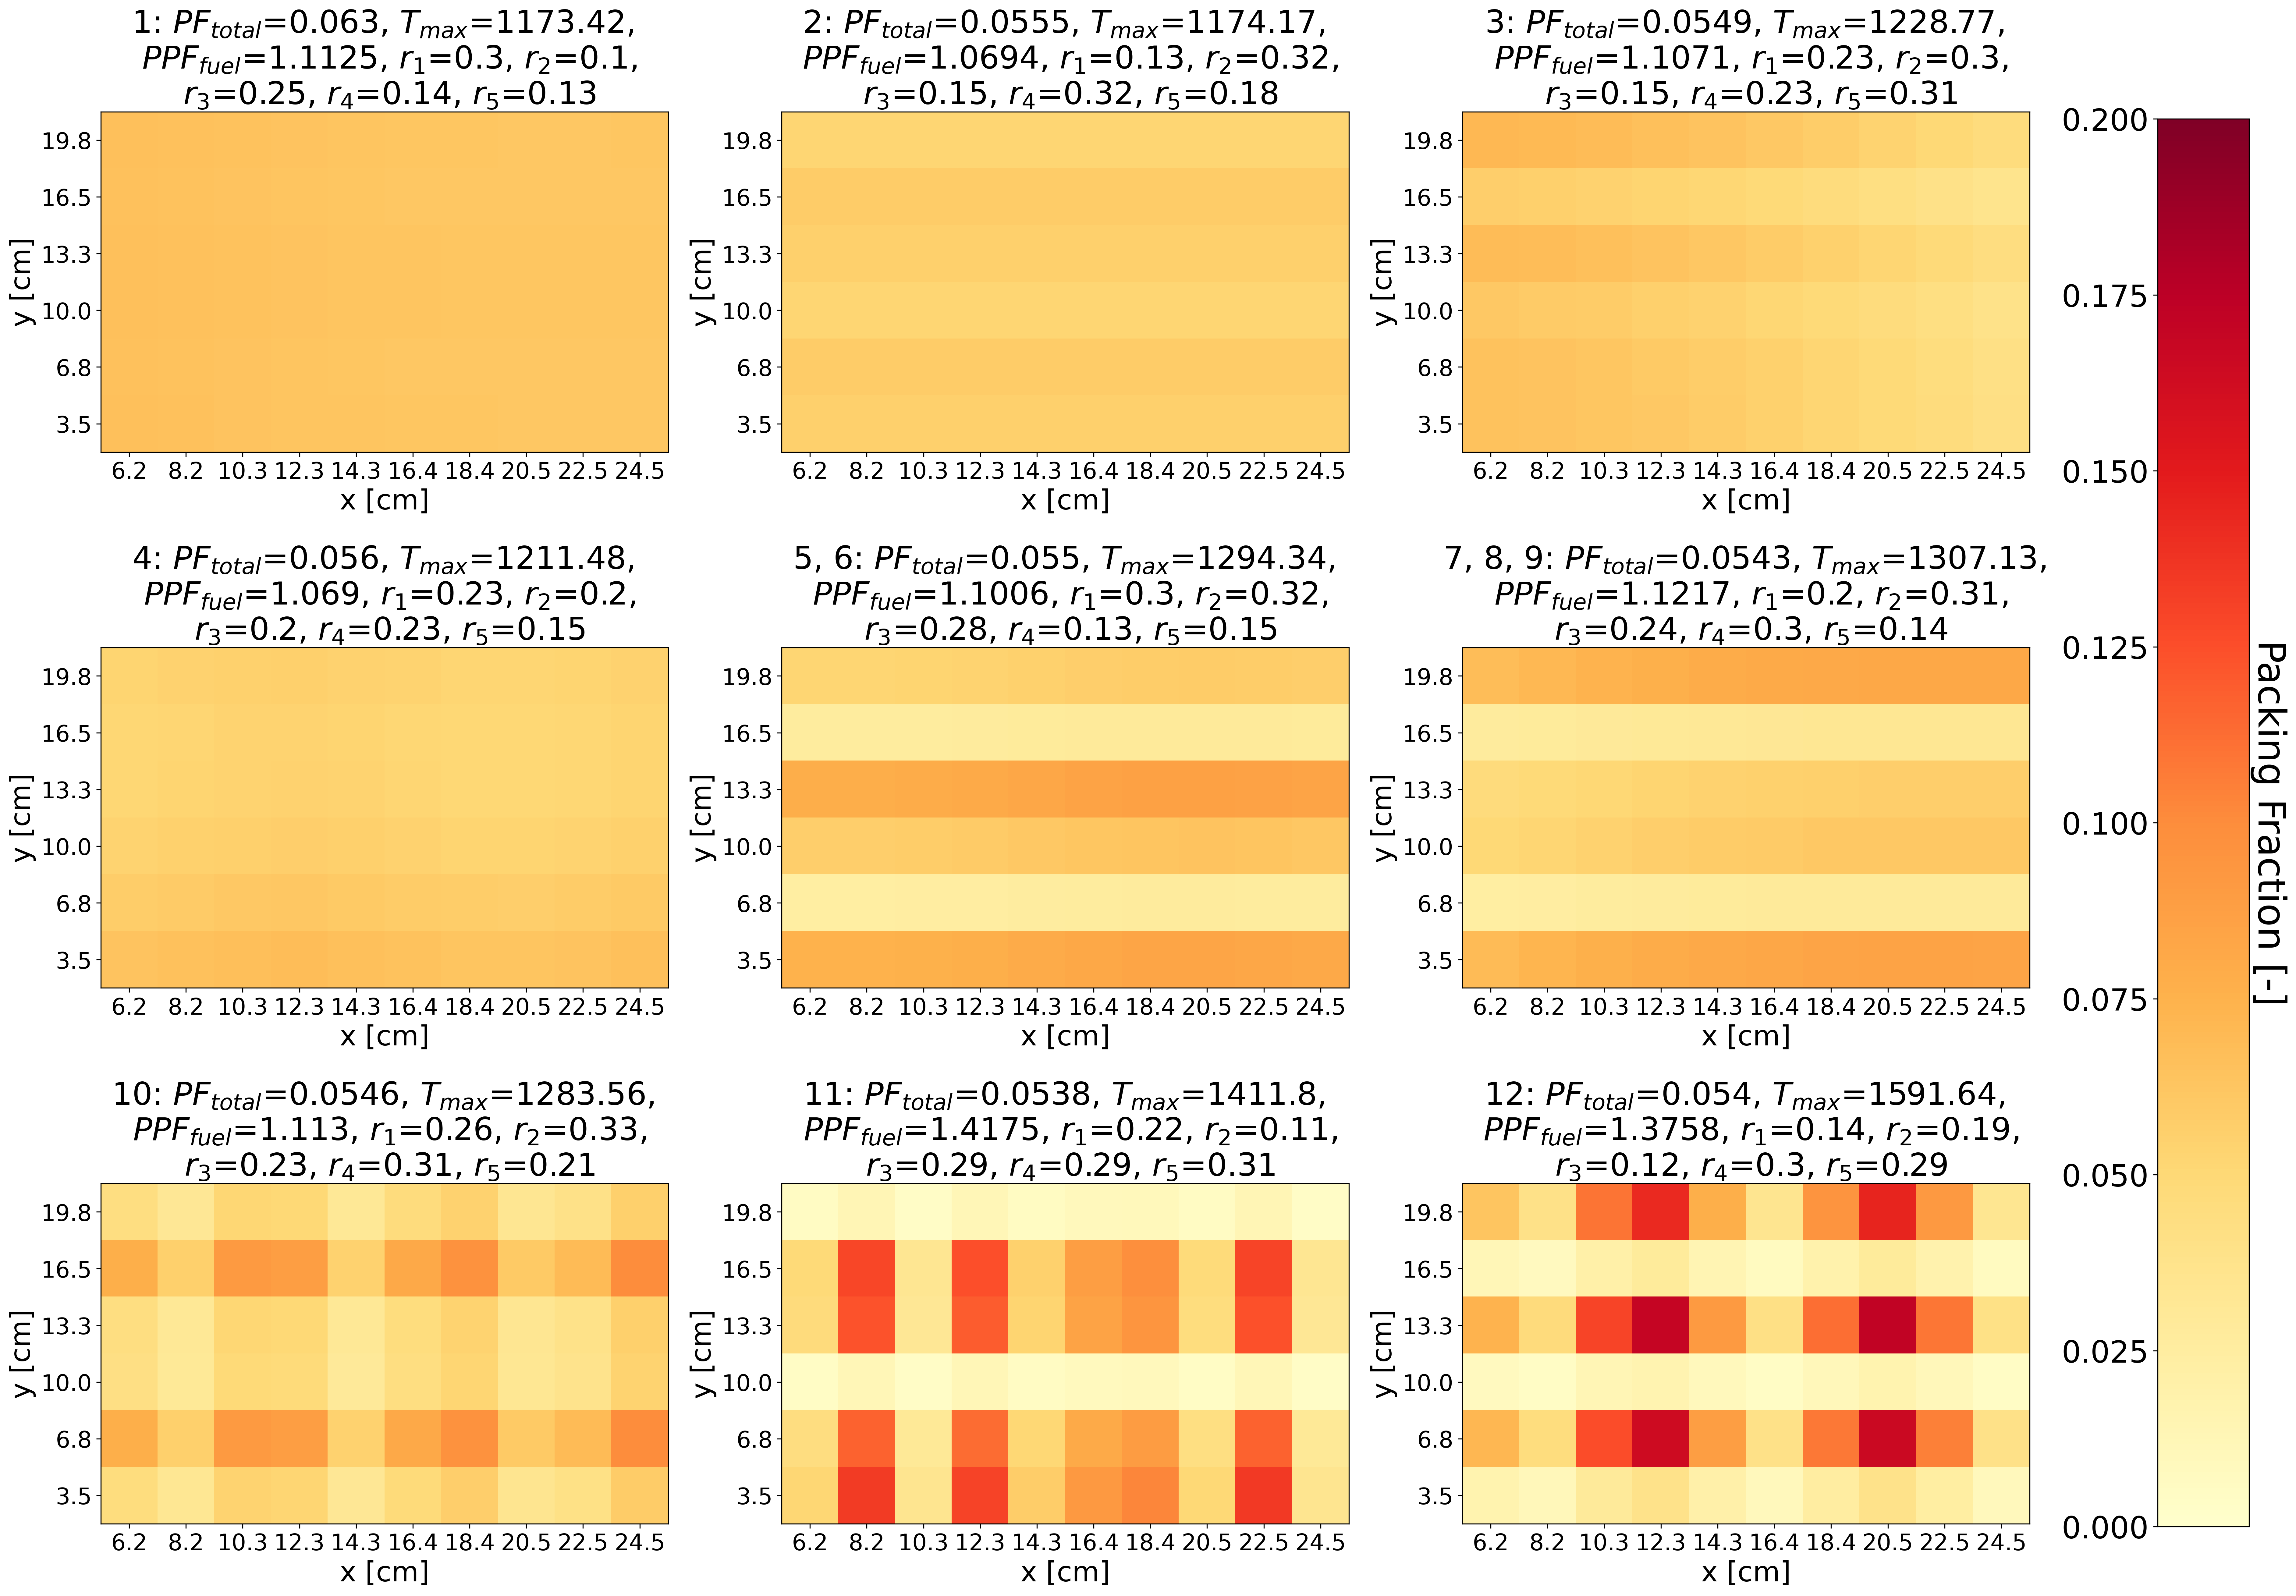
\includegraphics[width=\linewidth]{assem-obj-3-all-distr.png}
        \caption{TRISO distributions for the 12 reactor models on the Pareto front.
        Numbered reactor models correspond to numbered crosses in Figure 
        \ref{fig:assem-obj-3-all-2d}. }
        \label{fig:assem-obj-3-all-distr} 
    \end{subfigure}
    \caption{(contd.) Simulation a-3b -- ROLLO three-objective optimization to minimize 
    total fuel packing fraction ($PF_{total}$), maximum temperature ($T_{max}$), 
    and fuel-normalized power peaking factor ($PPF_{fuel}$) in the one-third assembly. 
    Input parameters varied: total fuel packing fraction $PF_{total}$, 
    TRISO packing fraction distribution ($\rho_{TRISO}(\vec{r})$), 
    coolant channel shape $(r_1, r_2, r_3, r_4, r_5)$.}
\end{figure}

Figure \ref{fig:assem-obj-3-all} demonstrates that \gls{ROLLO} found 12 reactor models 
on simulation a-3b final generation's Pareto front. 
Figure \ref{fig:assem-obj-3-all-most-minimized} shows three reactor models on the 
Pareto front that most-minimized each objective, and one reactor model on the 
Pareto front that equally minimized all three objectives. 
I selected the equally minimized reactor model by visually studying Figure 
\ref{fig:assem-obj-3-all} and selecting a reactor model that is close to the origin 
and has a light yellow color dimension. 
Reactor model 11 most-minimized $PF_{total}$, reactor model 1 most-minimized $T_{max}$, 
reactor model 4 most-minimized $PPF_{fuel}$, and reactor model 2 equally minimized 
all three objectives. 
\begin{figure}[htbp!]
    \centering
    \begin{subfigure}{\textwidth}
    \centering
    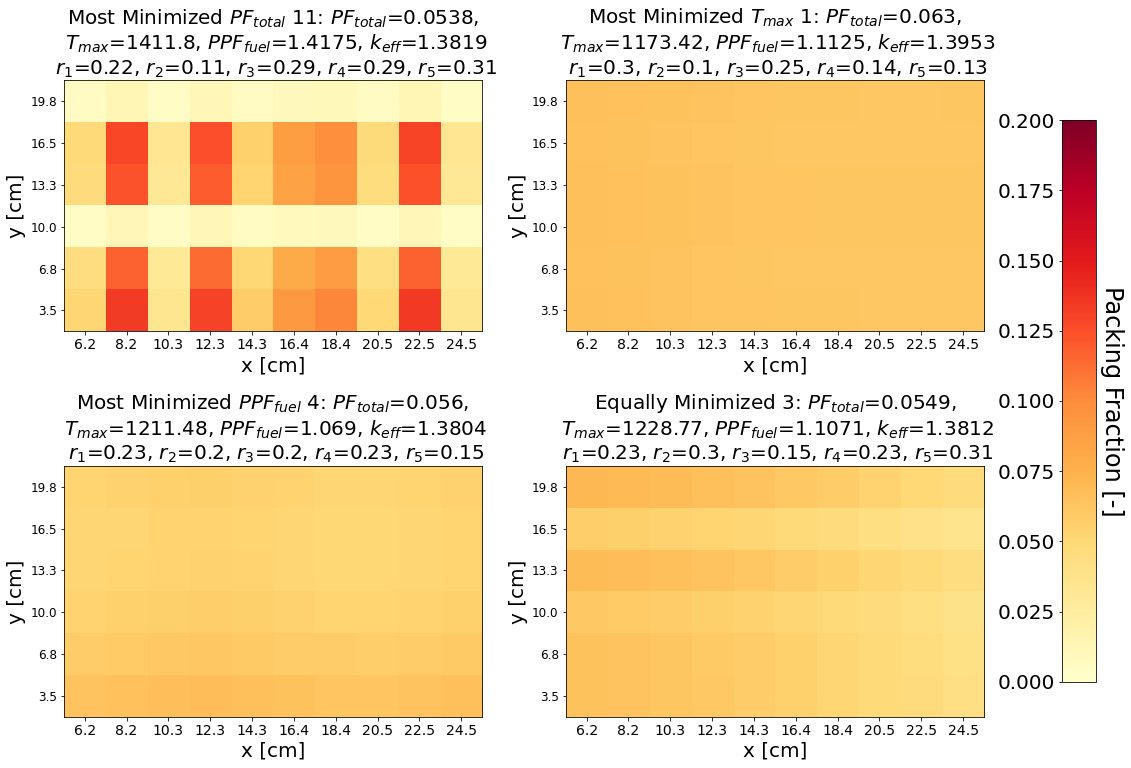
\includegraphics[width=\linewidth]{assem-obj-3-all-distr-most-minimized.png}
    \caption{TRISO packing fraction distributions.}
    \label{fig:assem-obj-3-all-most-minimized-distr}
    \end{subfigure}
    \caption{AHTR one-third assembly models and TRISO distributions for the 3 reactor 
    models on simulation a-3b's Pareto front that most-minimized each objective, and 
    1 reactor model that equally minimized all three objectives.
    Simulation a-3b -- ROLLO three-objective optimization to minimize 
    total fuel packing fraction ($PF_{total}$), maximum temperature ($T_{max}$), 
    and fuel-normalized power peaking factor ($PPF_{fuel}$) in the one-third assembly. 
    Input parameters varied: total fuel packing fraction $PF_{total}$, 
    TRISO packing fraction distribution ($\rho_{TRISO}(\vec{r})$), 
    coolant channel shape $(r_1, r_2, r_3, r_4, r_5)$.}
    \label{fig:assem-obj-3-all-most-minimized}
\end{figure}
\begin{figure}[htbp!]
    \ContinuedFloat
    \begin{subfigure}{0.49\textwidth}
        \centering
        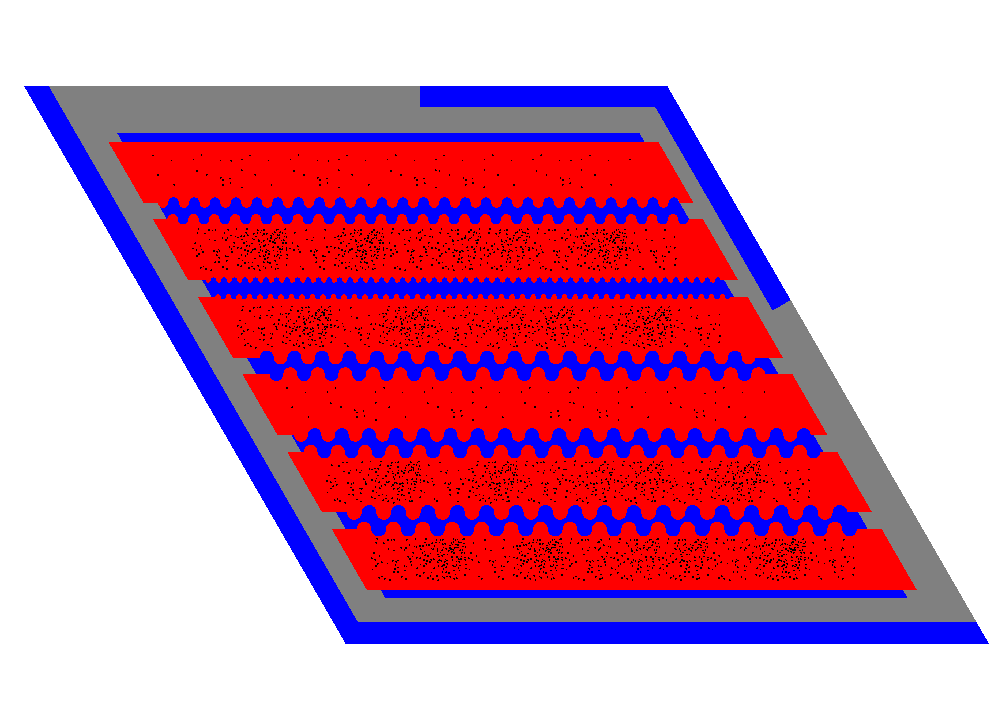
\includegraphics[width=\linewidth]{assem-obj-3-all-min-pf.png}
        \caption{\gls{AHTR} one-third assembly model with the most-minimized $PF_{total}$ 
        (reactor model 11).}
        \label{fig:assem-obj-3-all-min-pf} 
    \end{subfigure}
    \begin{subfigure}{0.49\textwidth}
        \centering
        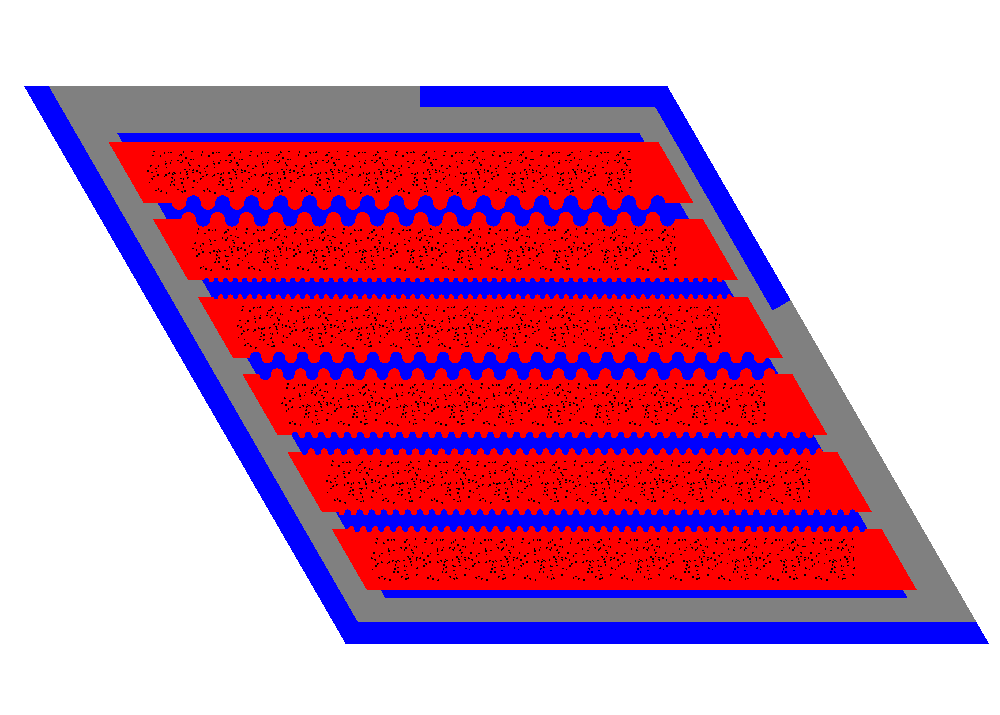
\includegraphics[width=\linewidth]{assem-obj-3-all-min-temp.png}
        \caption{\gls{AHTR} one-third assembly model with the most-minimized $T_{max}$
        (reactor model 1).}
        \label{fig:assem-obj-3-all-min-temp} 
    \end{subfigure}
    \begin{subfigure}{0.49\textwidth}
        \centering
        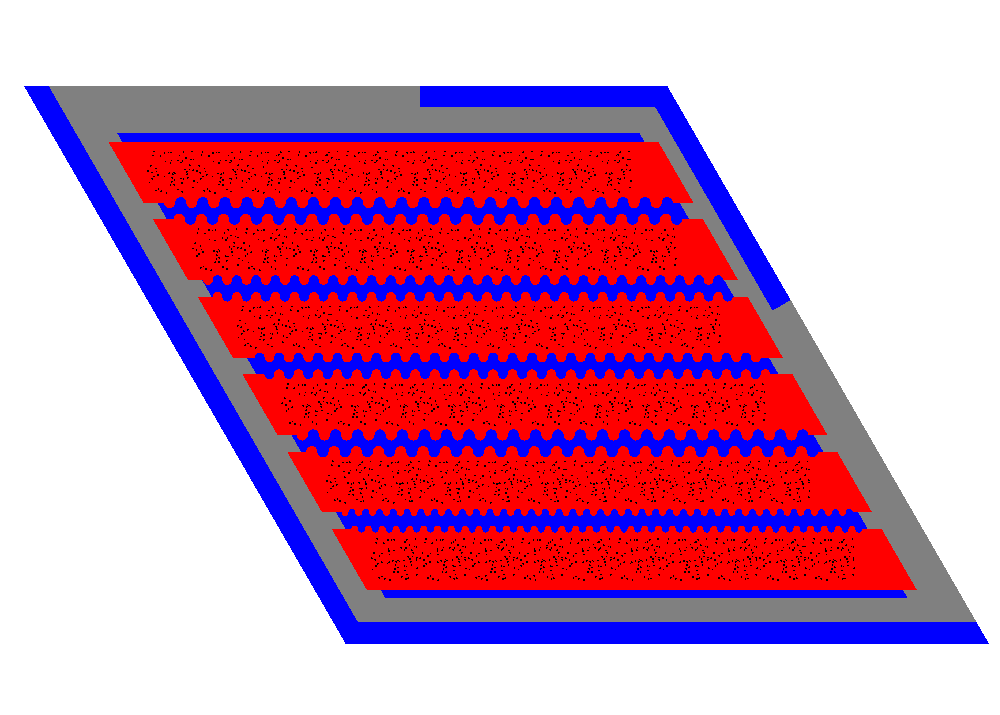
\includegraphics[width=\linewidth]{assem-obj-3-all-min-ppf.png}
        \caption{\gls{AHTR} one-third assembly model with the most-minimized $PPF_{fuel}$
        (reactor model 4).}
        \label{fig:assem-obj-3-all-min-ppf} 
    \end{subfigure}
    \begin{subfigure}{0.49\textwidth}
        \centering
        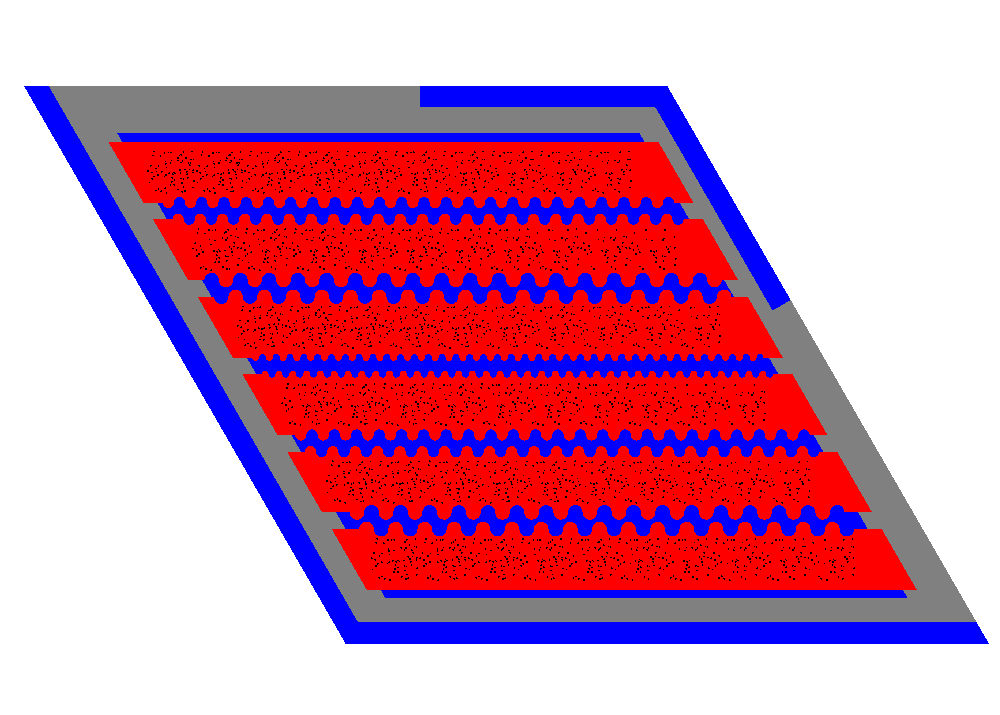
\includegraphics[width=\linewidth]{assem-obj-3-all-min-all.png}
        \caption{\gls{AHTR} one-third assembly model that equally minimized all 
        objectives (reactor model 3).}
        \label{fig:assem-obj-3-all-min-all} 
    \end{subfigure}
    \begin{subfigure}{.3\textwidth}
    \vspace{1cm}
    \centering
    \resizebox{\textwidth}{!}{
    \fbox{\begin{tabular}{ll}
        \textcolor{fhrblue}{$\blacksquare$} & \gls{FLiBe} \\
        \textcolor{fhrgrey}{$\blacksquare$} & Graphite (Structure)\\
        \textcolor{fhrred}{$\blacksquare$} & Graphite (Fuel Plank) \\
        \textcolor{fhrblack}{$\blacksquare$} & TRISO particle 
        \end{tabular}}}
\end{subfigure}
    \caption{(contd.) AHTR one-third assembly models and TRISO distributions for the 3 
    reactor models on simulation a-3b's Pareto front that most-minimized each 
    objective, and 1 reactor model that equally minimized all three objectives.
    Simulation a-3b -- ROLLO three-objective optimization to minimize 
    total fuel packing fraction ($PF_{total}$), maximum temperature ($T_{max}$), 
    and fuel-normalized power peaking factor ($PPF_{fuel}$) in the one-third assembly. 
    Input parameters varied: total fuel packing fraction $PF_{total}$, 
    TRISO packing fraction distribution ($\rho_{TRISO}(\vec{r})$), 
    coolant channel shape $(r_1, r_2, r_3, r_4, r_5)$.}
\end{figure}
% update equally minimized

In Figure \ref{fig:assem-obj-3-all-most-minimized-distr}, the one-third assembly model 
with the most-minimized $PF_{total}$ is reactor model 11 (also illustrated in Figure 
\ref{fig:assem-obj-3-all-min-pf}). 
Reactor model 11's TRISO distribution oscillates along the x-axis and slightly 
oscillates along the y-axis, and has a packing fraction standard deviation of 
$0.044$ across the one-third assembly. 
Along the x-axis, the distribution peaks at the 2nd and 9th fuel cell columns 
(at 8.2cm, 12.3cm, and 22.5cm), and minimum points at the 1st and 8th fuel cell 
columns (at 10.3cm and 24.5cm).
The 2nd and 9th columns have $\sim0.12$ y-axis variation with peaks of 
$PF\approx0.13$. 
The 1st and 8th columns have $\sim0.03$ y-axis variation with minimums of 
$PF\approx0.003$. 

In Figure \ref{fig:assem-obj-3-all-most-minimized-distr}, the one-third assembly model 
with the most-minimized $T_{max}$ is reactor model 1 (also illustrated in Figure 
\ref{fig:assem-obj-3-all-min-temp}). 
Reactor model 1 has an almost constant TRISO packing fraction distribution with 
a packing fraction standard deviation of $0.001$ across the one-third assembly. 
In Figure \ref{fig:assem-obj-3-all-most-minimized-distr}, the one-third assembly model 
with the most-minimized $PPF_{fuel}$ is reactor model 4 (also illustrated in Figure 
\ref{fig:assem-obj-3-all-min-ppf}). 
Reactor model 4's TRISO distribution oscillates slightly along the y-axis, and has a 
packing fraction standard deviation of $0.005$ across the one-third assembly. 
Along the y-axis, the distribution peaks at the 1st fuel cell row (at 3.5cm) with 
$PF\approx0.065$. 
The distribution has minimums at the 4th, 5th, and 6th fuel cell rows (at 13.3cm, 
16.5cm, and 19.8cm) with $PF\approx0.052$.

In Figure \ref{fig:assem-obj-3-all-most-minimized-distr}, the one-third assembly model 
that equally minimized all three objectives is reactor model 2 (also illustrated in 
Figure \ref{fig:assem-obj-3-all-min-all}).  
Reactor model 2's TRISO distribution oscillates slightly along the y-axis, and has a 
packing fraction standard deviation of $0.003$ across the one-third assembly.
Along the y-axis, the distribution peaks at the 2nd and 5th fuel cell row 
(at 6.8cm and 16.5cm) with $PF\approx0.058$. 
The distribution has minimums at the 3rd and 6th fuel cell rows (at 10.0cm and 19.8cm) 
with $PF\approx0.052$.
Section \ref{sec:assem-discussion-multi} discusses and explains simulation a-3b's 
results.

\section{AHTR One-Third Assembly: Computational Cost Summary}
\label{sec:assem-compute-cost}
Optimization simulations are run on the Theta supercomputer at the Argonne Leadership 
Computing Facility under the Director's Discretionary Allocation Program 
\cite{noauthor_argonne_2022}. 
Each Theta compute node has 64 processor cores with a nominal clock speed of 
1.5GHz \cite{noauthor_argonne_2022}.  

Each optimization simulation takes a different amount of node-hours to run due to 
differences in simulation software, tallies and intermediate steps required. 
Table \ref{tab:assem-compute-cost} reports the computational cost for each optimization 
simulation. 
Table \ref{tab:assem-obj-breakdown} detailed the simulation parameters.
\begin{table}[htbp!]
    \centering
    \onehalfspacing
    \caption{Computational cost of \acrfull{ROLLO} simulations for optimizing 
    \acrfull{AHTR} one-third assembly. BW: BlueWaters Supercomputer, Theta: Theta 
    supercomputer.}
	\label{tab:assem-compute-cost}
    \footnotesize
    \begin{tabular}{p{1.4cm}|p{1cm}lp{3.5cm}lp{3.5cm}}
        \hline 
        \textbf{Num of Objs} & \textbf{Sim} & \textbf{Machine} & 
        \textbf{Compute Cost Per Gen [node-hours]} &\textbf{Generations [\#]} & 
        \textbf{Total Compute Cost [node-hours]} \\
        \hline
    \multirow{6}{2cm}{1} 
    & a-1a & Theta &  95.3 & 3 & 285.8 \\
    & a-1b & Theta & 247.0 & 3 & 740.9 \\
    & a-1c & Theta & 115.0 & 2 & 230.0 \\
    & a-1d & Theta & 167.3 & 2 & 334.6 \\
    & a-1e & Theta & 346.1 & 2 & 692.3 \\
    & a-1f & Theta & 111.5 & 2 & 222.9 \\
    \hline
    \multirow{3}{2cm}{2}
    & a-2a & Theta & 250.2 & 5 & 1250.9 \\
    & a-2b & Theta &  98.3 & 5 &  491.7 \\
    & a-2c & Theta & 268.8 & 2 &  537.7 \\
    \hline
    \multirow{2}{2cm}{3}
    & a-3a & Theta & 273.6 & 5 & 1367.9 \\
    & a-3b & Theta & 305.8 & 5 & 1528.9 \\
    \hline
    \end{tabular}
\end{table}